% Options for packages loaded elsewhere
\PassOptionsToPackage{unicode}{hyperref}
\PassOptionsToPackage{hyphens}{url}
%
\documentclass[
]{book}
\usepackage{amsmath,amssymb}
\usepackage{lmodern}
\usepackage{iftex}
\ifPDFTeX
  \usepackage[T1]{fontenc}
  \usepackage[utf8]{inputenc}
  \usepackage{textcomp} % provide euro and other symbols
\else % if luatex or xetex
  \usepackage{unicode-math}
  \defaultfontfeatures{Scale=MatchLowercase}
  \defaultfontfeatures[\rmfamily]{Ligatures=TeX,Scale=1}
\fi
% Use upquote if available, for straight quotes in verbatim environments
\IfFileExists{upquote.sty}{\usepackage{upquote}}{}
\IfFileExists{microtype.sty}{% use microtype if available
  \usepackage[]{microtype}
  \UseMicrotypeSet[protrusion]{basicmath} % disable protrusion for tt fonts
}{}
\makeatletter
\@ifundefined{KOMAClassName}{% if non-KOMA class
  \IfFileExists{parskip.sty}{%
    \usepackage{parskip}
  }{% else
    \setlength{\parindent}{0pt}
    \setlength{\parskip}{6pt plus 2pt minus 1pt}}
}{% if KOMA class
  \KOMAoptions{parskip=half}}
\makeatother
\usepackage{xcolor}
\usepackage{color}
\usepackage{fancyvrb}
\newcommand{\VerbBar}{|}
\newcommand{\VERB}{\Verb[commandchars=\\\{\}]}
\DefineVerbatimEnvironment{Highlighting}{Verbatim}{commandchars=\\\{\}}
% Add ',fontsize=\small' for more characters per line
\usepackage{framed}
\definecolor{shadecolor}{RGB}{248,248,248}
\newenvironment{Shaded}{\begin{snugshade}}{\end{snugshade}}
\newcommand{\AlertTok}[1]{\textcolor[rgb]{0.94,0.16,0.16}{#1}}
\newcommand{\AnnotationTok}[1]{\textcolor[rgb]{0.56,0.35,0.01}{\textbf{\textit{#1}}}}
\newcommand{\AttributeTok}[1]{\textcolor[rgb]{0.77,0.63,0.00}{#1}}
\newcommand{\BaseNTok}[1]{\textcolor[rgb]{0.00,0.00,0.81}{#1}}
\newcommand{\BuiltInTok}[1]{#1}
\newcommand{\CharTok}[1]{\textcolor[rgb]{0.31,0.60,0.02}{#1}}
\newcommand{\CommentTok}[1]{\textcolor[rgb]{0.56,0.35,0.01}{\textit{#1}}}
\newcommand{\CommentVarTok}[1]{\textcolor[rgb]{0.56,0.35,0.01}{\textbf{\textit{#1}}}}
\newcommand{\ConstantTok}[1]{\textcolor[rgb]{0.00,0.00,0.00}{#1}}
\newcommand{\ControlFlowTok}[1]{\textcolor[rgb]{0.13,0.29,0.53}{\textbf{#1}}}
\newcommand{\DataTypeTok}[1]{\textcolor[rgb]{0.13,0.29,0.53}{#1}}
\newcommand{\DecValTok}[1]{\textcolor[rgb]{0.00,0.00,0.81}{#1}}
\newcommand{\DocumentationTok}[1]{\textcolor[rgb]{0.56,0.35,0.01}{\textbf{\textit{#1}}}}
\newcommand{\ErrorTok}[1]{\textcolor[rgb]{0.64,0.00,0.00}{\textbf{#1}}}
\newcommand{\ExtensionTok}[1]{#1}
\newcommand{\FloatTok}[1]{\textcolor[rgb]{0.00,0.00,0.81}{#1}}
\newcommand{\FunctionTok}[1]{\textcolor[rgb]{0.00,0.00,0.00}{#1}}
\newcommand{\ImportTok}[1]{#1}
\newcommand{\InformationTok}[1]{\textcolor[rgb]{0.56,0.35,0.01}{\textbf{\textit{#1}}}}
\newcommand{\KeywordTok}[1]{\textcolor[rgb]{0.13,0.29,0.53}{\textbf{#1}}}
\newcommand{\NormalTok}[1]{#1}
\newcommand{\OperatorTok}[1]{\textcolor[rgb]{0.81,0.36,0.00}{\textbf{#1}}}
\newcommand{\OtherTok}[1]{\textcolor[rgb]{0.56,0.35,0.01}{#1}}
\newcommand{\PreprocessorTok}[1]{\textcolor[rgb]{0.56,0.35,0.01}{\textit{#1}}}
\newcommand{\RegionMarkerTok}[1]{#1}
\newcommand{\SpecialCharTok}[1]{\textcolor[rgb]{0.00,0.00,0.00}{#1}}
\newcommand{\SpecialStringTok}[1]{\textcolor[rgb]{0.31,0.60,0.02}{#1}}
\newcommand{\StringTok}[1]{\textcolor[rgb]{0.31,0.60,0.02}{#1}}
\newcommand{\VariableTok}[1]{\textcolor[rgb]{0.00,0.00,0.00}{#1}}
\newcommand{\VerbatimStringTok}[1]{\textcolor[rgb]{0.31,0.60,0.02}{#1}}
\newcommand{\WarningTok}[1]{\textcolor[rgb]{0.56,0.35,0.01}{\textbf{\textit{#1}}}}
\usepackage{longtable,booktabs,array}
\usepackage{calc} % for calculating minipage widths
% Correct order of tables after \paragraph or \subparagraph
\usepackage{etoolbox}
\makeatletter
\patchcmd\longtable{\par}{\if@noskipsec\mbox{}\fi\par}{}{}
\makeatother
% Allow footnotes in longtable head/foot
\IfFileExists{footnotehyper.sty}{\usepackage{footnotehyper}}{\usepackage{footnote}}
\makesavenoteenv{longtable}
\usepackage{graphicx}
\makeatletter
\def\maxwidth{\ifdim\Gin@nat@width>\linewidth\linewidth\else\Gin@nat@width\fi}
\def\maxheight{\ifdim\Gin@nat@height>\textheight\textheight\else\Gin@nat@height\fi}
\makeatother
% Scale images if necessary, so that they will not overflow the page
% margins by default, and it is still possible to overwrite the defaults
% using explicit options in \includegraphics[width, height, ...]{}
\setkeys{Gin}{width=\maxwidth,height=\maxheight,keepaspectratio}
% Set default figure placement to htbp
\makeatletter
\def\fps@figure{htbp}
\makeatother
\setlength{\emergencystretch}{3em} % prevent overfull lines
\providecommand{\tightlist}{%
  \setlength{\itemsep}{0pt}\setlength{\parskip}{0pt}}
\setcounter{secnumdepth}{5}
\usepackage{booktabs}
\usepackage{amsthm}
\makeatletter
\def\thm@space@setup{%
  \thm@preskip=8pt plus 2pt minus 4pt
  \thm@postskip=\thm@preskip
}
\makeatother
\usepackage{booktabs}
\usepackage{longtable}
\usepackage{array}
\usepackage{multirow}
\usepackage{wrapfig}
\usepackage{float}
\usepackage{colortbl}
\usepackage{pdflscape}
\usepackage{tabu}
\usepackage{threeparttable}
\usepackage{threeparttablex}
\usepackage[normalem]{ulem}
\usepackage{makecell}
\usepackage{xcolor}
\ifLuaTeX
  \usepackage{selnolig}  % disable illegal ligatures
\fi
\usepackage[]{natbib}
\bibliographystyle{plainnat}
\IfFileExists{bookmark.sty}{\usepackage{bookmark}}{\usepackage{hyperref}}
\IfFileExists{xurl.sty}{\usepackage{xurl}}{} % add URL line breaks if available
\urlstyle{same} % disable monospaced font for URLs
\hypersetup{
  pdftitle={Statistics Tutorials \& Templates},
  pdfauthor={Dr.~F.J. Rodenburg © 2022},
  hidelinks,
  pdfcreator={LaTeX via pandoc}}

\title{Statistics Tutorials \& Templates}
\author{Dr.~F.J. Rodenburg © 2022}
\date{}

\begin{document}
\maketitle

{
\setcounter{tocdepth}{1}
\tableofcontents
}
\hypertarget{preface}{%
\chapter*{Preface}\label{preface}}
\addcontentsline{toc}{chapter}{Preface}

This website contains tutorials and templates for statistical analysis in R markdown. It is primarily meant as reference material for the \href{https://fransrodenburg.github.io/General-Research-Skills/}{statistics course} taught at the Institute of Biology Leiden, Leiden University.

\textbf{This is not a general reference for how to do statistical analysis.} That cannot be done concisely for a number of reasons:

\begin{itemize}
\tightlist
\item
  The right analysis depends on the goal of the study. Is the study exploratory? Is there a predefined hypothesis to be tested? Is the main goal prediction? Is the main goal (causal) inference? Has the study been properly designed for this goal?
\item
  Phenomena that complicate typical analysis. Usually, a substantial part of analysis involves data cleaning, getting the data in \href{https://r4ds.had.co.nz/tidy-data.html\#fig:tidy-structure}{tidy format}, dealing with \href{https://en.wikipedia.org/wiki/Missing_data\#Types}{missing data}, and identifying any number of other potentially complicating factors (censoring, zero-inflation, etc.).
\item
  Limitations of \href{https://en.wikipedia.org/wiki/Statistical_inference\#Paradigms_for_inference}{frequentist statistics}.
\item
  Limitations of \emph{any} supposedly exhaustive list of techniques. If your problem does not easily fall into one of the categories of analysis shown here, I recommend you consult with a statistician.
\end{itemize}

Finally, please note that this page is meant to show you how to \emph{do} things, not how statistical methods work. For that, please refer to our free online material over \href{https://fransrodenburg.github.io/General-Research-Skills/}{here}.

\begin{center}\rule{0.5\linewidth}{0.5pt}\end{center}

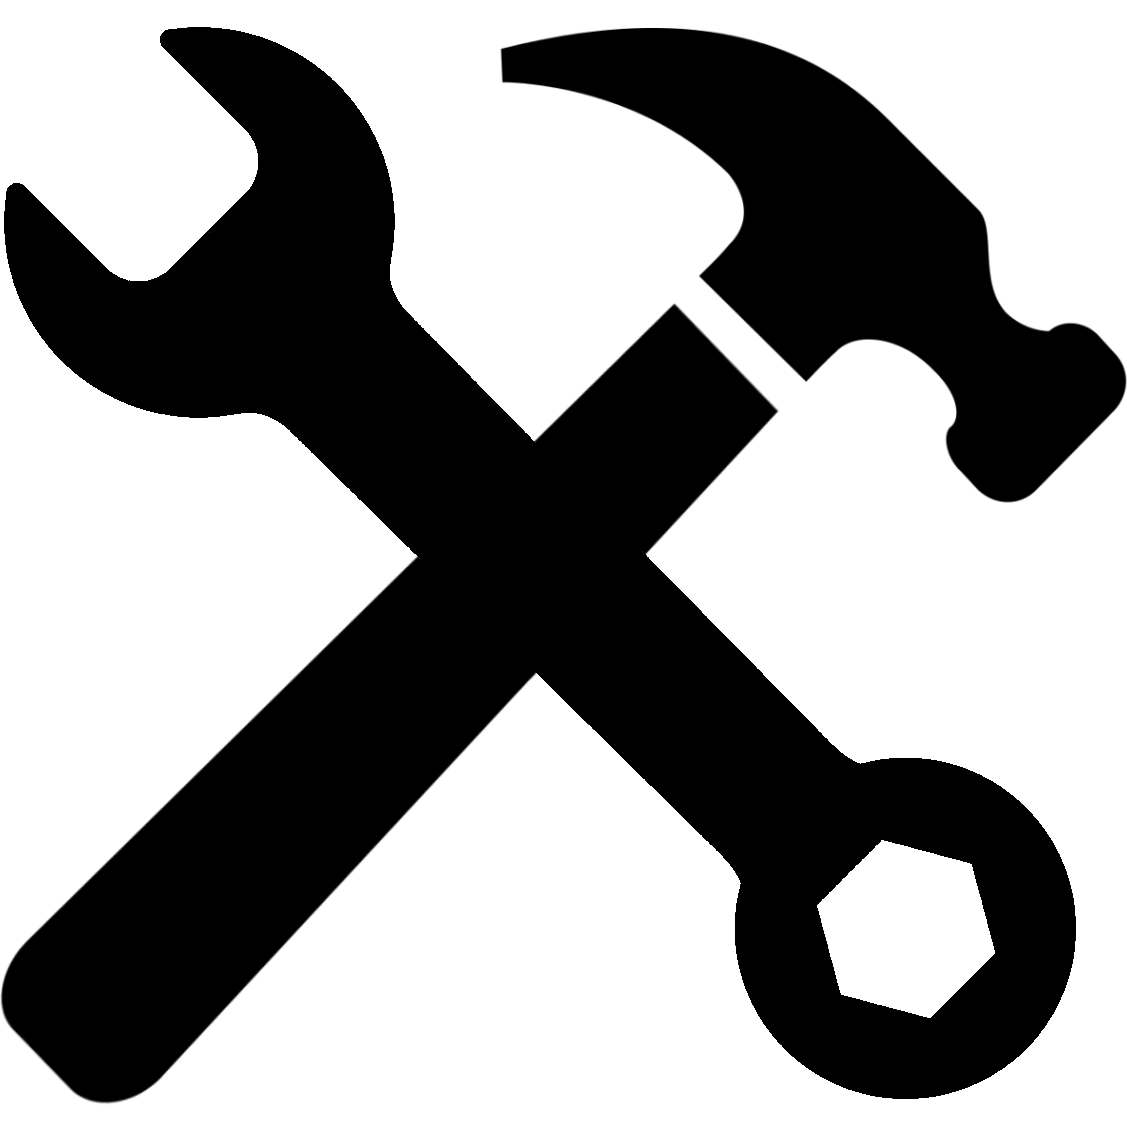
\includegraphics[width=0.20833in,height=0.20833in]{figures/underconstruction.png} The tutorials website is a work in progress. Please check back later for updates.

\hypertarget{t-test}{%
\chapter{T-Test}\label{t-test}}

A hypothesis test to compare two means to see if they differ significantly. Assumptions depend on the type of \(t\)-test.

\begin{center}\rule{0.5\linewidth}{0.5pt}\end{center}

Summary

\begin{enumerate}
\def\labelenumi{\arabic{enumi}.}
\tightlist
\item
  \href{https://youtu.be/BGUqZc-Pb8w}{Read the data into R };
\item
  Visualize the data;
\item
  Choose an appropriate \href{https://youtu.be/qJA3CvFt_pc}{type of \(t\)-test };
\item
  Report a conclusion;
\item
  Incorporating this in scientific literature.
\end{enumerate}

You can download the tutorial \href{files/tutorial_t-test.Rmd}{here} and the required data set \href{data/two-groups.csv}{here}.

\hypertarget{read-t}{%
\section{Read the Data into R}\label{read-t}}

I recommend saving data as \href{https://youtu.be/BGUqZc-Pb8w}{comma-separated values (CSV)}. If you prefer reading data directly from Excel, have a look \protect\hyperlink{Excel}{here}.

Details

\begin{itemize}
\tightlist
\item
  Save the data in a folder;
\item
  Open RStudio and create a new R markdown file; (\textbf{File} \textgreater{} \textbf{New File} \textgreater{} \textbf{R Markdown})
\item
  Save your R markdown file to the same location as the data;
\item
  Set working directory to source file location. (\textbf{Session} \textgreater{} \textbf{Set Working Directory} \textgreater{} \textbf{To Source File Location})
\end{itemize}

\begin{Shaded}
\begin{Highlighting}[]
\NormalTok{DF }\OtherTok{\textless{}{-}} \FunctionTok{read.csv}\NormalTok{(}\StringTok{"two{-}groups.csv"}\NormalTok{)}
\end{Highlighting}
\end{Shaded}

Did that work? There are several ways to check:

\begin{Shaded}
\begin{Highlighting}[]
\FunctionTok{str}\NormalTok{(DF)}
\FunctionTok{summary}\NormalTok{(DF)}
\FunctionTok{head}\NormalTok{(DF)}
\end{Highlighting}
\end{Shaded}

Explanation of the output

\begin{Shaded}
\begin{Highlighting}[]
\FunctionTok{str}\NormalTok{(DF)}
\end{Highlighting}
\end{Shaded}

\begin{verbatim}
## 'data.frame':    60 obs. of  3 variables:
##  $ X        : int  1 2 3 4 5 6 7 8 9 10 ...
##  $ Pesticide: chr  "A" "A" "A" "A" ...
##  $ CropYield: num  101.5 98.9 105.9 100.9 101 ...
\end{verbatim}

This command shows the structure of the data. It is a data frame with \(n = 60\) observations and 2 variables. \texttt{Pesticide} is a character vector (\texttt{chr}) and \texttt{CropYield} a numeric vector (\texttt{num}).

\begin{verbatim}
##        X          Pesticide           CropYield     
##  Min.   : 1.00   Length:60          Min.   : 92.90  
##  1st Qu.:15.75   Class :character   1st Qu.: 98.08  
##  Median :30.50   Mode  :character   Median : 99.85  
##  Mean   :30.50                      Mean   : 99.96  
##  3rd Qu.:45.25                      3rd Qu.:101.55  
##  Max.   :60.00                      Max.   :105.90
\end{verbatim}

\begin{verbatim}
##   X Pesticide CropYield
## 1 1         A     101.5
## 2 2         A      98.9
## 3 3         A     105.9
## 4 4         A     100.9
## 5 5         A     101.0
## 6 6         A     100.4
\end{verbatim}

My output looks different

Then provided you did everything else correctly, the most likely reason is that your data was saved with a version of Excel where a comma is used as a decimal separator (e.g., the Dutch version). The solutions for this is simple, use \texttt{read.csv2}:

\begin{Shaded}
\begin{Highlighting}[]
\NormalTok{DF }\OtherTok{\textless{}{-}} \FunctionTok{read.csv2}\NormalTok{(}\StringTok{"some{-}data{-}with{-}commas.csv"}\NormalTok{)}
\end{Highlighting}
\end{Shaded}

If that doesn't work either, go over the details shown above, or watch the instructions in the \href{https://youtu.be/BGUqZc-Pb8w}{video}.

Common mistakes

\begin{itemize}
\tightlist
\item
  Remember to include the file extension (e.g., ``two-groups\textbf{.csv}'') when typing the file name.
\item
  You cannot read Excel files (.xls, .xlsx) with this function. Instead, follow the guide \protect\hyperlink{read}{here}, or save your data as CSV.
\item
  Don't open the CSV file with Excel. You don't need Excel or Google Sheets or any other program besides R and RStudio. If you have saved your data as CSV, you can close Excel.
\end{itemize}

The next step is to ensure categorical variables are read as factors. This will allow us to use generic functions like \texttt{plot} and \texttt{summary} in a more meaningful way.

Why not just use \texttt{character}?

A character vector is just strings of text, numbers and/or symbols. If you were to produce a \texttt{summary}, this happens:

\begin{Shaded}
\begin{Highlighting}[]
\FunctionTok{summary}\NormalTok{(DF}\SpecialCharTok{$}\NormalTok{Pesticide)}
\end{Highlighting}
\end{Shaded}

\begin{verbatim}
##    Length     Class      Mode 
##        60 character character
\end{verbatim}

It tells us this object contains 60 values, and it is stored and treated as a string of text.

The generic \texttt{plot} function doesn't even work at all:

\begin{Shaded}
\begin{Highlighting}[]
\FunctionTok{plot}\NormalTok{(CropYield }\SpecialCharTok{\textasciitilde{}}\NormalTok{ Pesticide, DF)}
\end{Highlighting}
\end{Shaded}

\begin{verbatim}
Error in plot.window(...) : need finite 'xlim' values
In addition: Warning messages:
1: In xy.coords(x, y, xlabel, ylabel, log) : NAs introduced by coercion
2: In min(x) : no non-missing arguments to min; returning Inf
3: In max(x) : no non-missing arguments to max; returning -Inf
\end{verbatim}

Now convert the variables to factors and see how that changes the output. \emph{(Run the code below, then run \texttt{summary(DF\$Pesticide)}, or \texttt{plot(DF\$Pesticide)} for example.)}

\begin{Shaded}
\begin{Highlighting}[]
\NormalTok{DF}\SpecialCharTok{$}\NormalTok{Pesticide }\OtherTok{\textless{}{-}} \FunctionTok{factor}\NormalTok{(DF}\SpecialCharTok{$}\NormalTok{Pesticide)}
\end{Highlighting}
\end{Shaded}

\hypertarget{vis-t}{%
\section{Visualize the Data}\label{vis-t}}

There are different ways to go about this. A basic, but still very popular choice is the boxplot:

\begin{Shaded}
\begin{Highlighting}[]
\FunctionTok{boxplot}\NormalTok{(CropYield }\SpecialCharTok{\textasciitilde{}}\NormalTok{ Pesticide, DF)}
\end{Highlighting}
\end{Shaded}

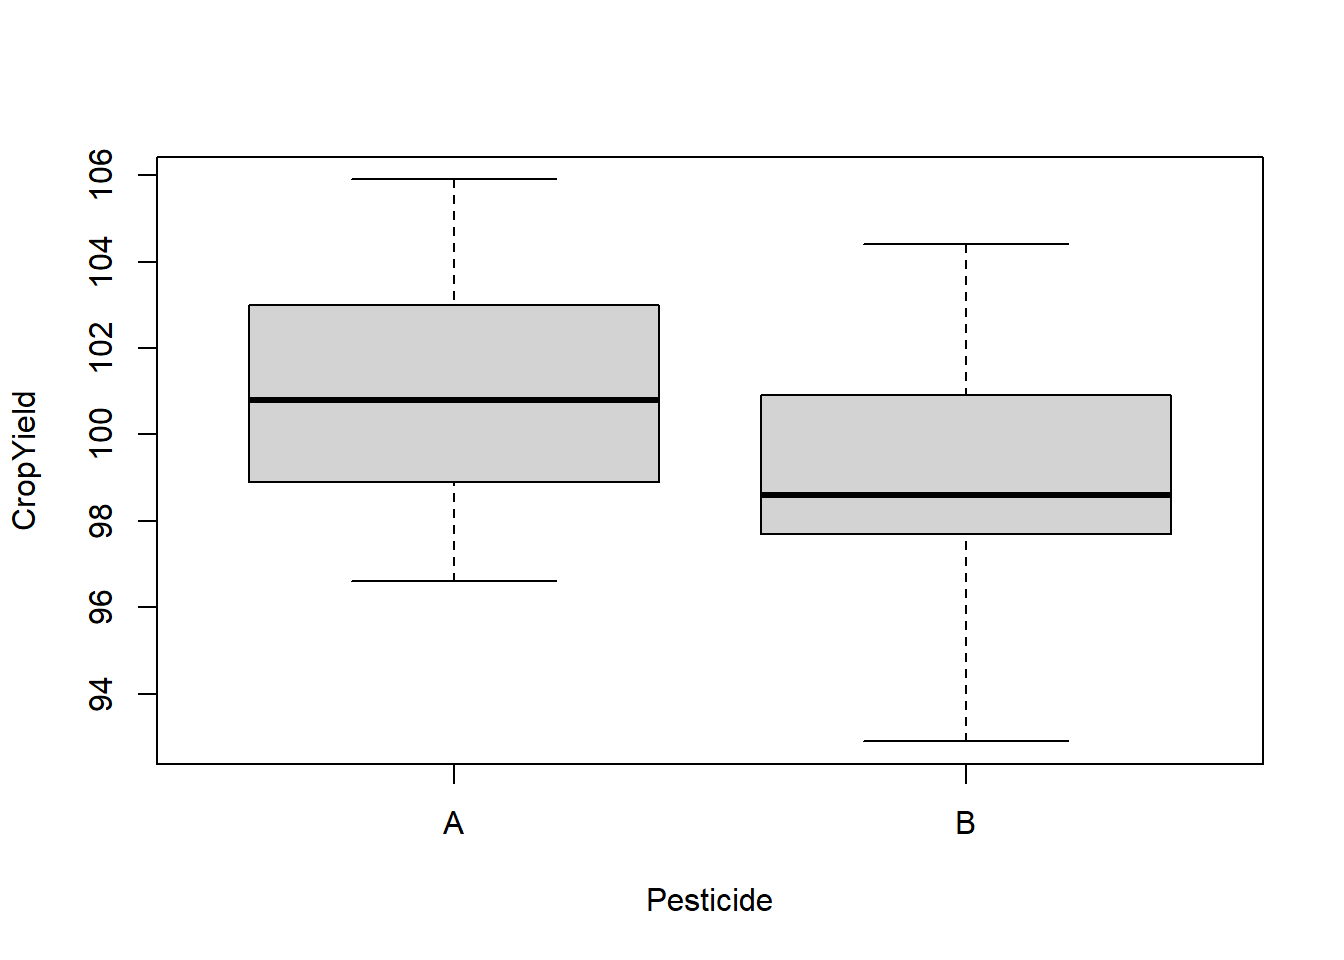
\includegraphics{Tutorials_files/figure-latex/unnamed-chunk-10-1.pdf}

What to look for

Potential Outliers

A boxplot shows either of the following:

\begin{figure}
\centering
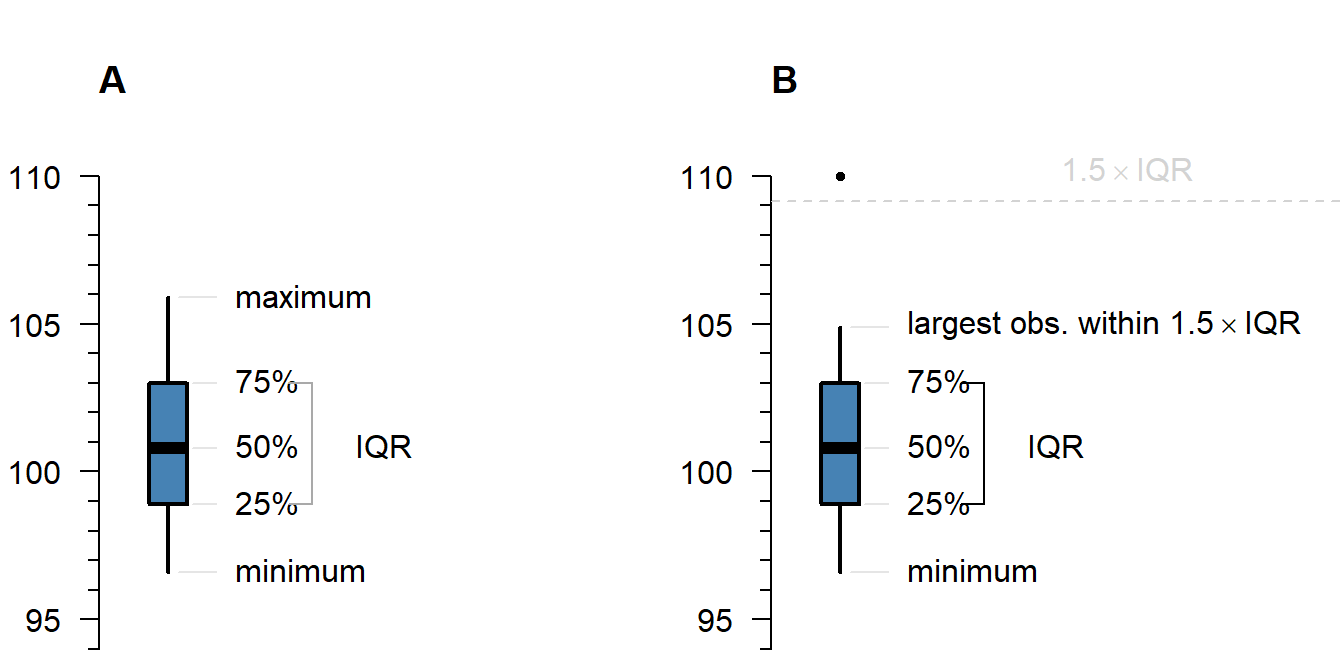
\includegraphics{Tutorials_files/figure-latex/IQR-1.pdf}
\caption{\label{fig:IQR}What is displayed in a boxplot in case all observations are within a certain distance from the box (A), or otherwise (B).}
\end{figure}

The interquartile range (IQR) is simply the size of the box. If all observations lie within \(1.5\times\) this range from the box, then the whiskers show the extremes of the data (fig.~\ref{fig:IQR} A). Otherwise, the observations are drawn separately \ref{fig:IQR} B). The IQR is usually not shown in a boxplot, but is used internally to calculate the location of the whiskers and marked observations (if any).

Marked observations are not outliers

This is a common misconception. Though it can be an \emph{indication} of outlyingness, a boxplot alone cannot tell you whether these observations will strongly affect your analysis:

\begin{itemize}
\tightlist
\item
  If you have a large enough sample size, you \emph{will} find more extreme observations, which are eventually drawn outside the IQR.
\item
  Skewed values (see next section) will almost always show `outliers' in the direction of skew, but these are unlikely to be outliers in the context of an appropriate model for skewed data.
\item
  The \(1.5\times\) IQR rule is nothing special, it is merely convention. A boxplot is just a quick way to visualize numeric values.
\end{itemize}

Skew

Skew means the data-generating process follows a probability distribution that is not symmetric. In a boxplot, skew looks like this:

\begin{figure}
\centering
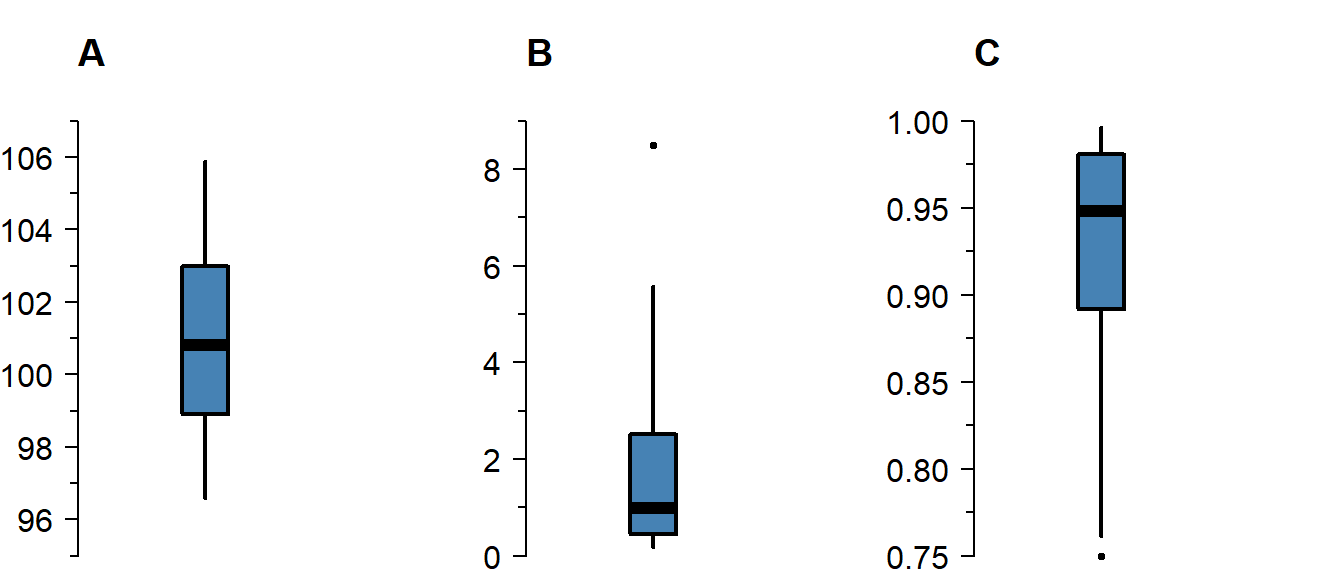
\includegraphics{Tutorials_files/figure-latex/skew-1.pdf}
\caption{\label{fig:skew}A boxplot of symmetric (A), right-skewed (B), and left-skewed values.}
\end{figure}

Skew is not necessarily a problem, unless it persists in the residuals of a model that assumes normally distributed errors. For an explanation of skew, see the video on \href{https://youtu.be/jdfG7rKPVNk}{probability distributions }.

Differences Between Groups

A boxplot is not just a nice tool for \emph{yourself} to inspect your data, but is also an effective tool to visually communicate the evidence for difference between groups:

\begin{figure}
\centering
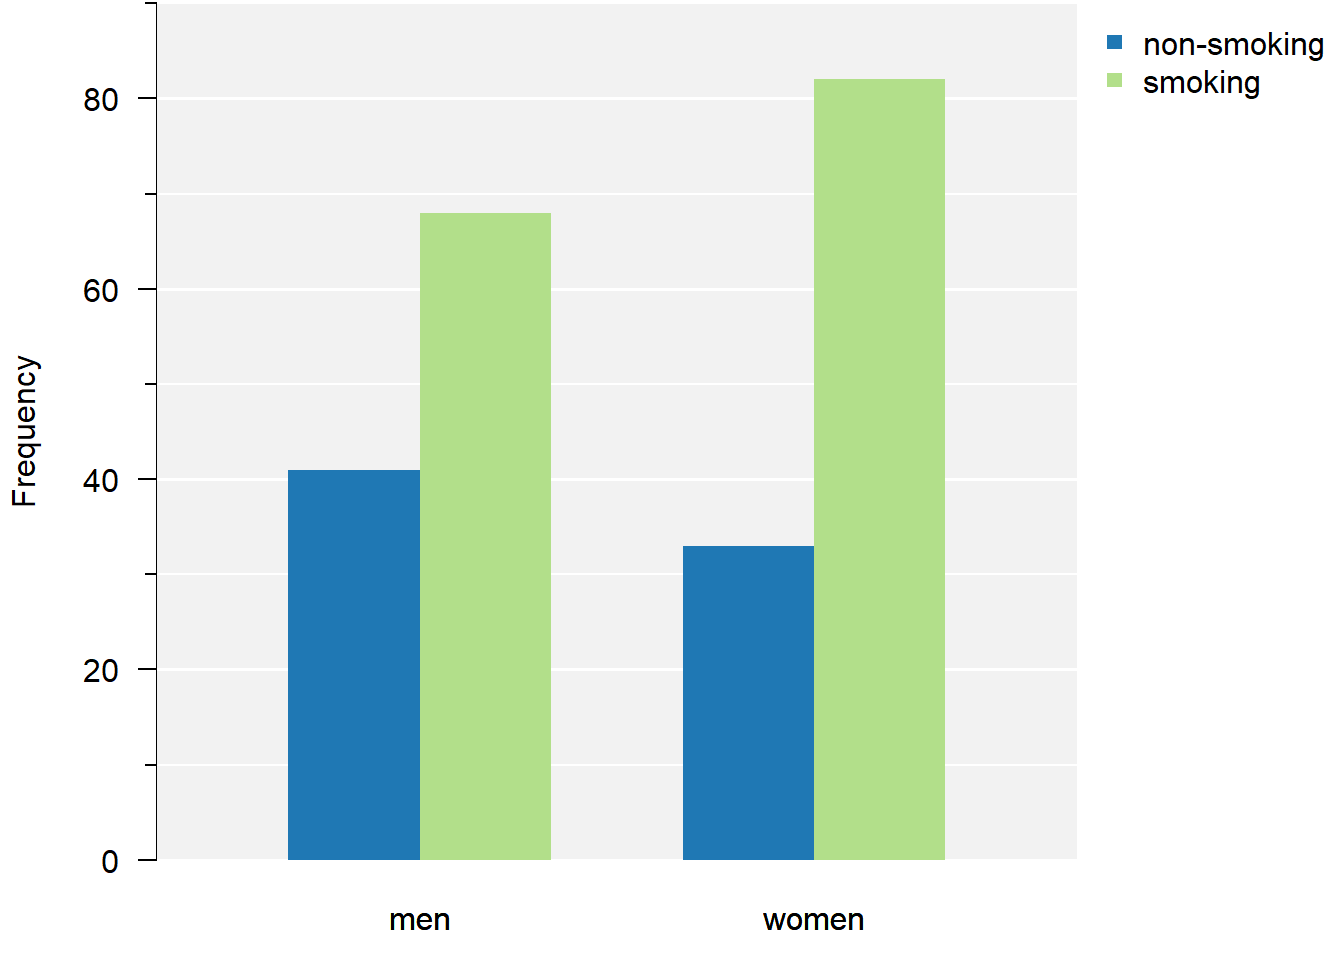
\includegraphics{Tutorials_files/figure-latex/unnamed-chunk-11-1.pdf}
\caption{\label{fig:unnamed-chunk-11}A comparison of crop yield for pesticides A and B.}
\end{figure}

From the plot you can conclude:

\begin{itemize}
\tightlist
\item
  Neither group appears to have outliers;
\item
  Neither group appears skewed;
\item
  Pesticide A seems to yield more crop than B, but there is considerable overlap;
\item
  The variance of both groups is similar, because the boxes are similarly sized.
\end{itemize}

This is just a sample, so whether this difference is \emph{significant}, should be determined with a test.

How to improve your plot

Some basic adjustments that improve any plot:

\begin{itemize}
\tightlist
\item
  Use informative axis labels, with unit of measurement if appropriate;
\item
  Add an informative caption;
\item
  Keep the numbers on the axes horizontal where possible;
\item
  Remove unnecessary plot elements, like the box around the figure.
\end{itemize}

The changes to the code I made below can all be found in the help pages \texttt{?boxplot} and \texttt{?par}. I am also a big fan of the \texttt{eaxis} function from the package \texttt{sfsmisc}. The caption is added as a chunk option (i.e., \texttt{\textasciigrave{}\textasciigrave{}\textasciigrave{}\{r,\ fig.cap\ =\ "..."\}}).

\begin{Shaded}
\begin{Highlighting}[]
\CommentTok{\# Load a package for nice axes}
\FunctionTok{library}\NormalTok{(}\StringTok{"sfsmisc"}\NormalTok{)}

\CommentTok{\# Change the margins (bottom, left, top, right)}
\FunctionTok{par}\NormalTok{(}\AttributeTok{mar =} \FunctionTok{c}\NormalTok{(}\DecValTok{4}\NormalTok{, }\DecValTok{4}\NormalTok{, }\DecValTok{0}\NormalTok{, }\DecValTok{0}\NormalTok{) }\SpecialCharTok{+} \FloatTok{0.1}\NormalTok{)}

\CommentTok{\# Create the coordinate system}
\FunctionTok{boxplot}\NormalTok{(CropYield }\SpecialCharTok{\textasciitilde{}}\NormalTok{ Pesticide, DF, }\AttributeTok{axes =} \ConstantTok{FALSE}\NormalTok{, }\AttributeTok{boxwex =} \FloatTok{0.25}\NormalTok{, }\AttributeTok{staplewex =} \DecValTok{0}\NormalTok{,}
        \AttributeTok{ylab =} \StringTok{"Crop yield (kg)"}\NormalTok{, }\AttributeTok{ylim =} \FunctionTok{c}\NormalTok{(}\DecValTok{92}\NormalTok{, }\DecValTok{108}\NormalTok{), }\AttributeTok{lwd =} \DecValTok{2}\NormalTok{, }\AttributeTok{lty =} \DecValTok{1}\NormalTok{)}

\CommentTok{\# Add axes}
\FunctionTok{axis}\NormalTok{(}\DecValTok{1}\NormalTok{, }\DecValTok{1}\SpecialCharTok{:}\DecValTok{2}\NormalTok{, }\FunctionTok{c}\NormalTok{(}\StringTok{"A"}\NormalTok{, }\StringTok{"B"}\NormalTok{))}
\FunctionTok{eaxis}\NormalTok{(}\DecValTok{2}\NormalTok{)}

\CommentTok{\# Add a lightgrey background}
\FunctionTok{polygon}\NormalTok{(}\AttributeTok{x =} \FunctionTok{c}\NormalTok{(}\SpecialCharTok{{-}}\DecValTok{1}\NormalTok{, }\DecValTok{3}\NormalTok{, }\DecValTok{3}\NormalTok{, }\SpecialCharTok{{-}}\DecValTok{1}\NormalTok{, }\SpecialCharTok{{-}}\DecValTok{1}\NormalTok{), }\AttributeTok{y =} \FunctionTok{c}\NormalTok{(}\DecValTok{90}\NormalTok{, }\DecValTok{90}\NormalTok{, }\DecValTok{110}\NormalTok{, }\DecValTok{110}\NormalTok{, }\DecValTok{90}\NormalTok{), }\AttributeTok{col =} \StringTok{"grey95"}\NormalTok{)}

\CommentTok{\# Add a simple grid}
\FunctionTok{abline}\NormalTok{(}\AttributeTok{h =} \FunctionTok{seq}\NormalTok{(}\DecValTok{90}\NormalTok{, }\DecValTok{110}\NormalTok{, }\DecValTok{1}\NormalTok{), }\AttributeTok{col =} \StringTok{"white"}\NormalTok{, }\AttributeTok{lwd =} \DecValTok{1}\NormalTok{)}
\FunctionTok{abline}\NormalTok{(}\AttributeTok{h =} \FunctionTok{seq}\NormalTok{(}\DecValTok{90}\NormalTok{, }\DecValTok{110}\NormalTok{, }\DecValTok{2}\NormalTok{), }\AttributeTok{col =} \StringTok{"white"}\NormalTok{, }\AttributeTok{lwd =} \FloatTok{1.5}\NormalTok{)}

\CommentTok{\# Redraw the boxplots on top}
\FunctionTok{boxplot}\NormalTok{(CropYield }\SpecialCharTok{\textasciitilde{}}\NormalTok{ Pesticide, DF, }\AttributeTok{axes =} \ConstantTok{FALSE}\NormalTok{, }\AttributeTok{boxwex =} \FloatTok{0.25}\NormalTok{, }\AttributeTok{staplewex =} \DecValTok{0}\NormalTok{,}
        \AttributeTok{col =} \StringTok{"steelblue"}\NormalTok{, }\AttributeTok{add =} \ConstantTok{TRUE}\NormalTok{, }\AttributeTok{lwd =} \DecValTok{2}\NormalTok{, }\AttributeTok{lty =} \DecValTok{1}\NormalTok{)}

\CommentTok{\# Restore the default margins for subsequent plots}
\FunctionTok{par}\NormalTok{(}\AttributeTok{mar =} \FunctionTok{c}\NormalTok{(}\DecValTok{5}\NormalTok{, }\DecValTok{4}\NormalTok{, }\DecValTok{4}\NormalTok{, }\DecValTok{3}\NormalTok{) }\SpecialCharTok{+} \FloatTok{0.1}\NormalTok{)}
\end{Highlighting}
\end{Shaded}

\begin{figure}
\centering
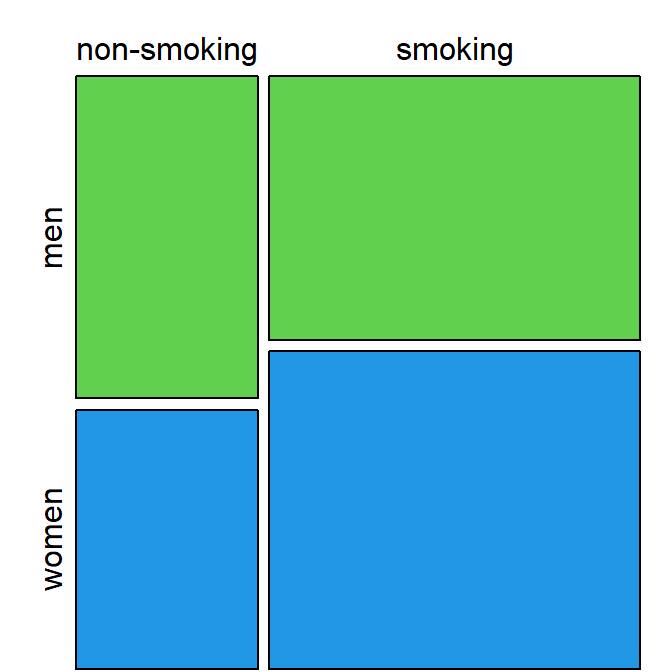
\includegraphics{Tutorials_files/figure-latex/unnamed-chunk-13-1.pdf}
\caption{\label{fig:unnamed-chunk-13}A comparison of crop yield for pesticides A and B.}
\end{figure}

Alternative: Violin plot

A more modern take on the boxplot is a \textbf{violin plot}. It combines a boxplot and a density plot. This type of visualization is richer in information than just a boxplot, but it is only meaningful if you have enough observations per group (e.g., \textgreater10):

\begin{Shaded}
\begin{Highlighting}[]
\FunctionTok{library}\NormalTok{(}\StringTok{"vioplot"}\NormalTok{) }\CommentTok{\# install if missing}
\FunctionTok{vioplot}\NormalTok{(CropYield }\SpecialCharTok{\textasciitilde{}}\NormalTok{ Pesticide, DF)}
\end{Highlighting}
\end{Shaded}

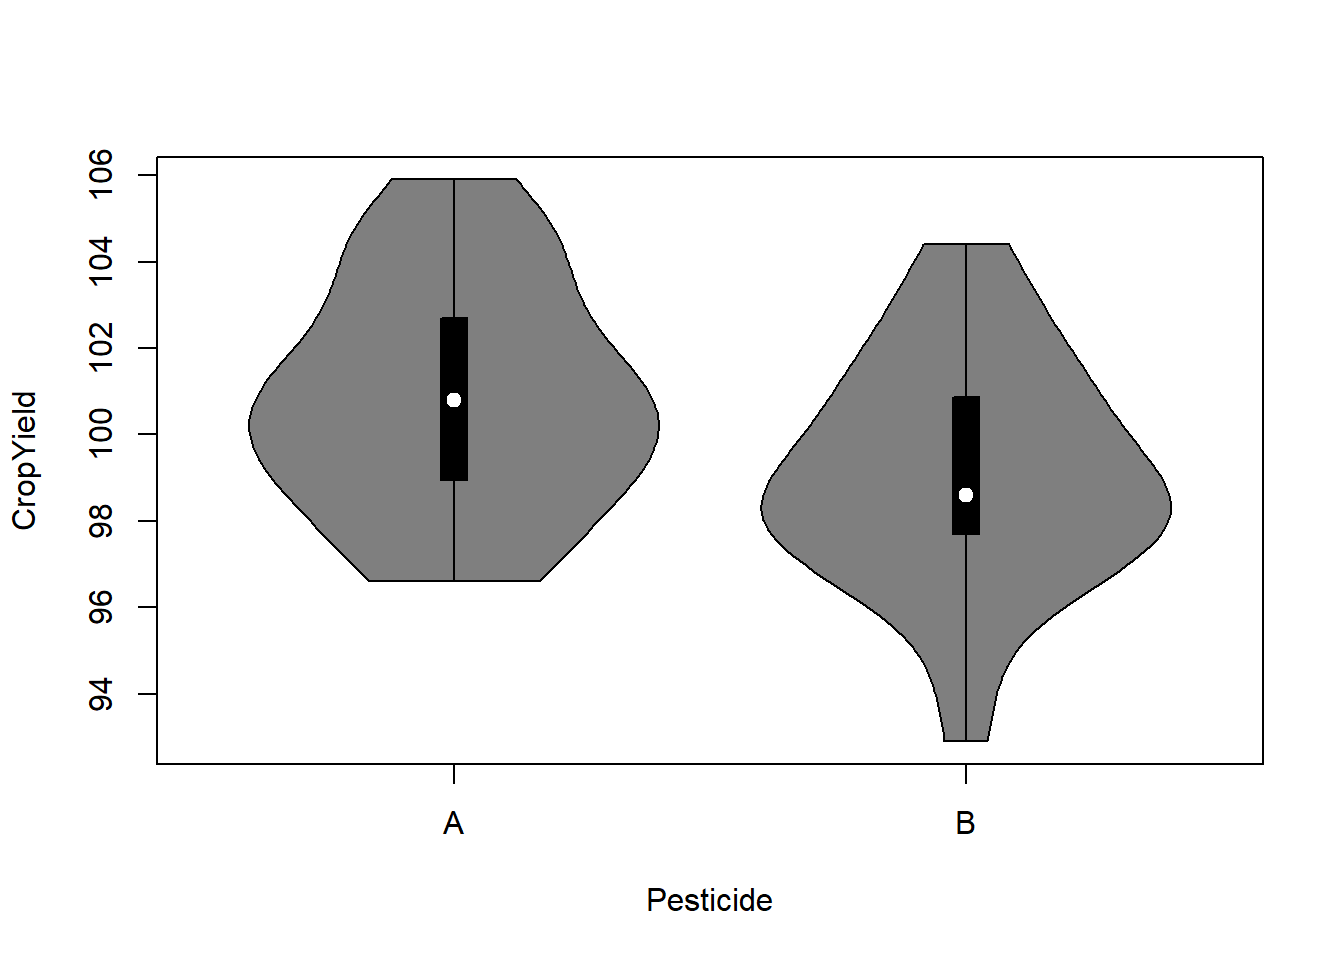
\includegraphics{Tutorials_files/figure-latex/unnamed-chunk-14-1.pdf}

How to interpret a violin plot

Here is a breakdown of the components shown in a violin plot:

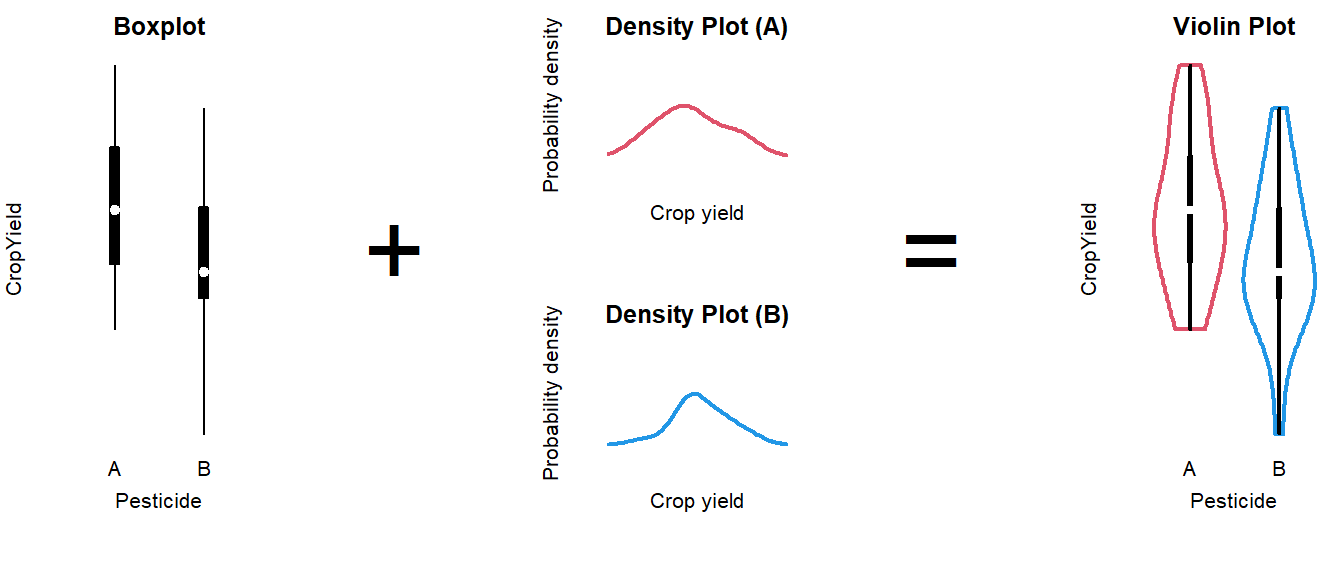
\includegraphics{Tutorials_files/figure-latex/unnamed-chunk-15-1.pdf}

The density plot, if you are unfamiliar with it, is like a continuous version of a histogram. It shows which values are more and less likely in the sample.

\hypertarget{choose-an-appropriate-t-test}{%
\section{Choose an Appropriate T-Test}\label{choose-an-appropriate-t-test}}

This part is still a work in progress. Refer to the \href{https://youtu.be/qJA3CvFt_pc}{video } for now.

One-sided or two-sided

You can test in two directions: Either the mean of A is greater than that of B, or the other way around. If you test for both possibilities, the test is called two-sided. Below is a short summary of the possibilities.

\begin{table}

\caption{\label{tab:unnamed-chunk-16}The directions in which you can test and the corresponding null-hypothesis.}
\centering
\fontsize{13}{15}\selectfont
\begin{tabular}[t]{l|l|l|l}
\hline
Type & Question & Syntax & Null-hypothesis\\
\hline
two-sided & Is there a difference in group means? & `t.test(..., alternative = "two.sided"` & $H_0: \mu_A \neq \mu_B$\\
\hline
one-sided & Is the mean of A greater than that of B? & `t.test(..., alternative = "greater"` & $H_0: \mu_A \leq \mu_B$\\
\hline
one-sided & Is the mean of A less than that of B? & `t.test(..., alternative = "less"` & $H_0: \mu_A \geq \mu_B$\\
\hline
\end{tabular}
\end{table}

A one-sided test is more powerful than a two-sided test. For instance, if you want to know whether a treatment yields \emph{lower} blood pressure than a control group, you should use a one-sided test.

If you test one-sided, you have to be able to defend this choice without seeing the data, or any plots. If you are unsure, test \emph{two-sided}.

Equal or unequal variance

\begin{figure}
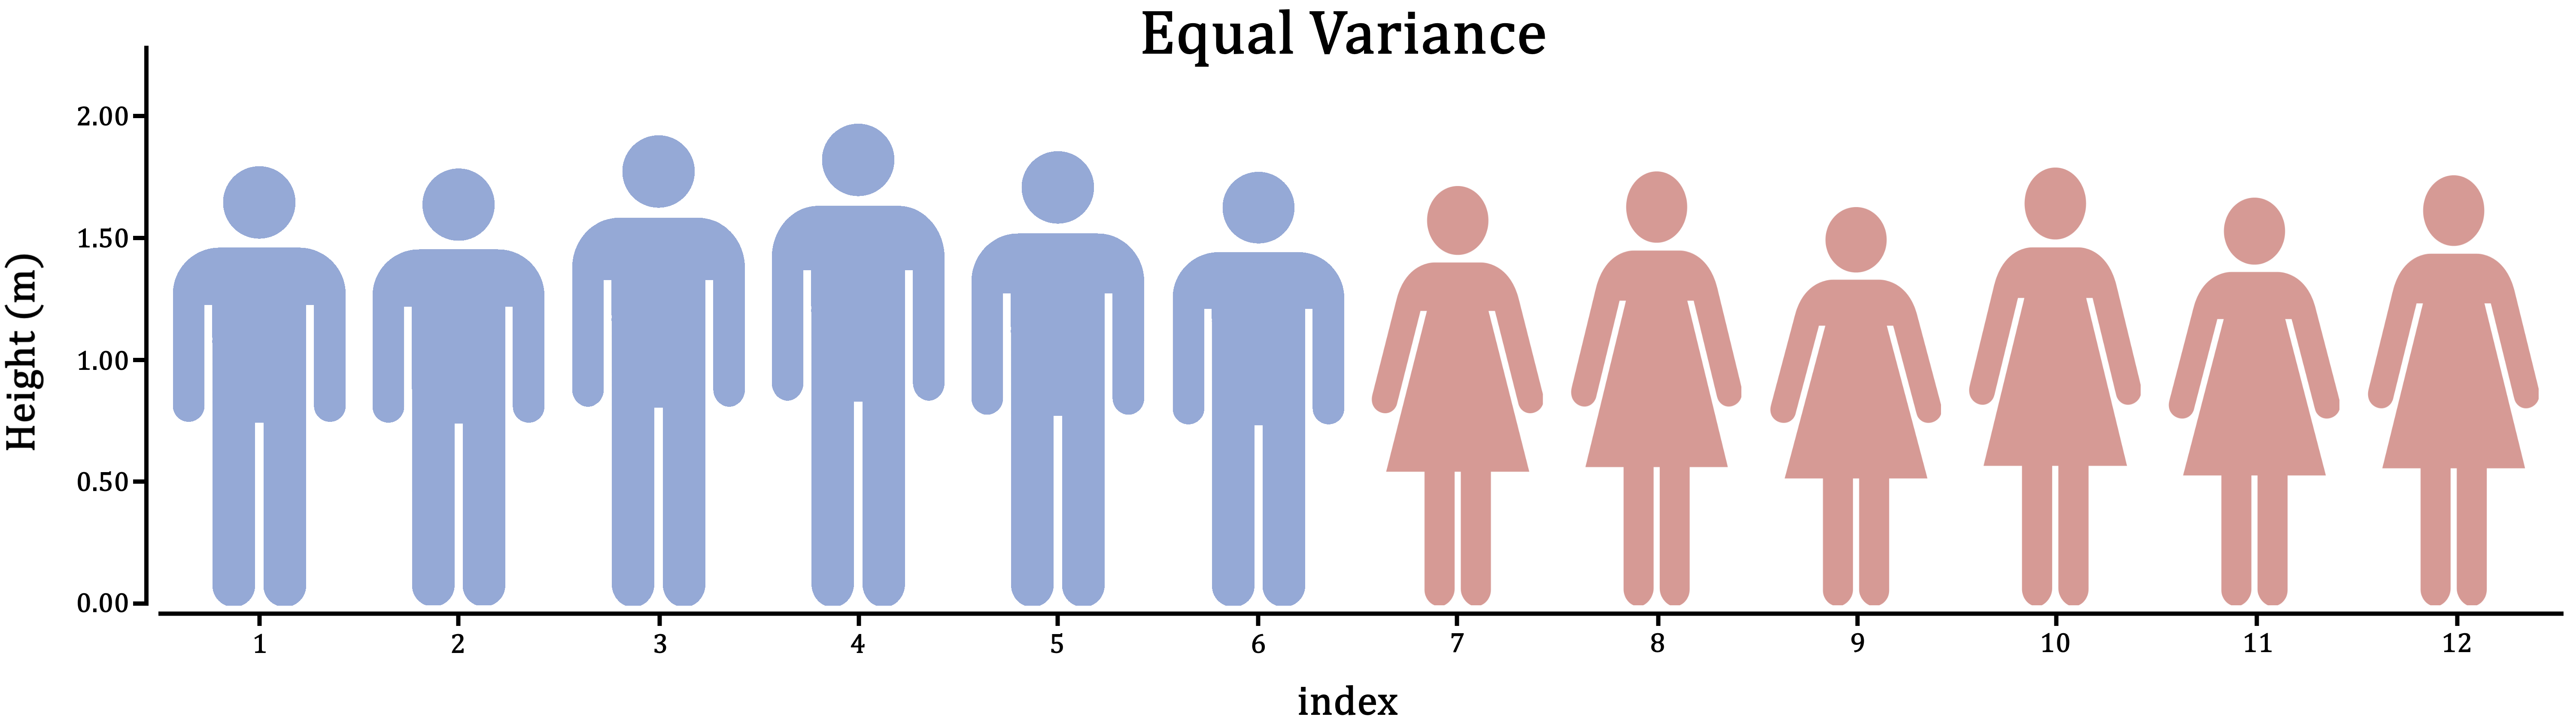
\includegraphics[width=0.75\linewidth]{figures/sexHeight2} 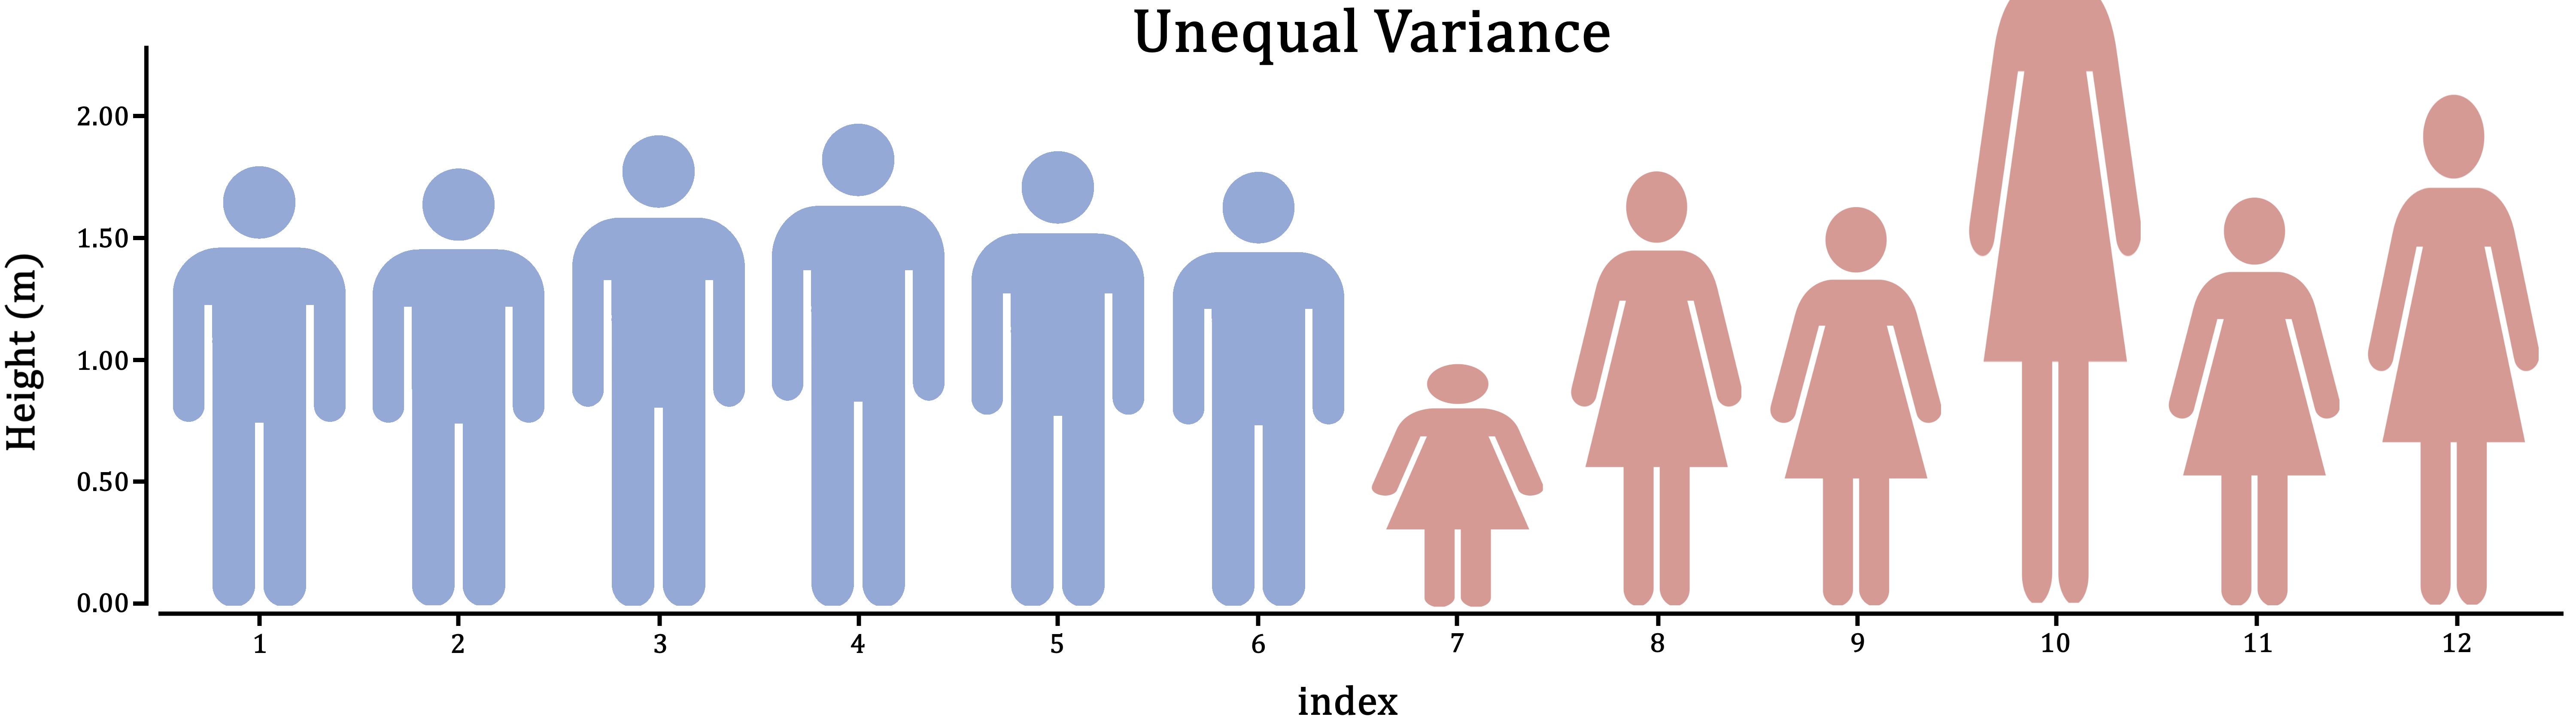
\includegraphics[width=0.75\linewidth]{figures/unequalVariance2} \caption{Variance is the extent to which individuals differ from their group mean. In the case of male and female human height, which do you think is more realistic?}\label{fig:unnamed-chunk-17}
\end{figure}

First, think about it in the context of the research: Does it make sense for these groups to vary to the same extent; should they have similar individual differences?

If you can't think of the right answer to that question, the safer of the two assumptions is \emph{unequal} variance. This will estimate a variance for both groups separately, at the cost of some power.

From the \protect\hyperlink{vis-t}{boxplot} we could already tell that the group variances are more or less equal in the example. In cases where it isn't obvious, you could conduct an \(F\)-test:

\begin{Shaded}
\begin{Highlighting}[]
\FunctionTok{var.test}\NormalTok{(CropYield }\SpecialCharTok{\textasciitilde{}}\NormalTok{ Pesticide, DF)}
\end{Highlighting}
\end{Shaded}

\begin{verbatim}
## 
##  F test to compare two variances
## 
## data:  CropYield by Pesticide
## F = 1.0152, num df = 29, denom df = 29, p-value = 0.9678
## alternative hypothesis: true ratio of variances is not equal to 1
## 95 percent confidence interval:
##  0.4832202 2.1330227
## sample estimates:
## ratio of variances 
##           1.015244
\end{verbatim}

In this case, the ratio \(\frac{\text{Var}(A)}{\text{Var}(B)} \approx 1\) (\texttt{1.015244}), with a \(p\)-value of \texttt{0.9678}, indicating the variances do not differ significantly.

\emph{(If these values came from populations with equal variance, you would have a \(96.8\%\) chance of drawing a sample with at least this large a difference in variance. This chance is very large, so we do not reject the null-hypothesis.)}

One-sample \(t\)-test

It is also possible to compare a single group mean to a fixed point. For example, does the temperature in class rooms differ significantly from 20\(^\circ\)C?

You can do this in R as follows:

\begin{Shaded}
\begin{Highlighting}[]
\CommentTok{\# Measurements from 7 class rooms}
\NormalTok{Temp }\OtherTok{\textless{}{-}} \FunctionTok{c}\NormalTok{(}\DecValTok{24}\NormalTok{, }\DecValTok{19}\NormalTok{, }\DecValTok{19}\NormalTok{, }\DecValTok{23}\NormalTok{, }\DecValTok{19}\NormalTok{, }\DecValTok{22}\NormalTok{, }\DecValTok{22}\NormalTok{)}

\CommentTok{\# Do these measurements differ from an average of 20 degrees?}
\FunctionTok{t.test}\NormalTok{(Temp, }\AttributeTok{mu =} \DecValTok{20}\NormalTok{)}
\end{Highlighting}
\end{Shaded}

\begin{verbatim}
## 
##  One Sample t-test
## 
## data:  Temp
## t = 1.4292, df = 6, p-value = 0.2029
## alternative hypothesis: true mean is not equal to 20
## 95 percent confidence interval:
##  19.18616 23.09955
## sample estimates:
## mean of x 
##  21.14286
\end{verbatim}

In this example, there is insufficient evidence to conclude a difference from 20\(^\circ\)C (95\% CI: 19.2--23.1).

Paired \(t\)-test

\ldots{}

Non-parametric alternative

\ldots{}

The advantage of this approach is that we use all observations (both A and B) at once to assess the assumptions. This is especially helpful when you only have a small number of observations in both groups, because diagnostics on small sample sizes is largely guesswork.

In the example shown here, the appropriate choice would be an independent, two-sample, two-sided, equal variance \(t\)-test:

\begin{Shaded}
\begin{Highlighting}[]
\FunctionTok{t.test}\NormalTok{(CropYield }\SpecialCharTok{\textasciitilde{}}\NormalTok{ Pesticide, }\AttributeTok{data =}\NormalTok{ DF, }\AttributeTok{var.equal =} \ConstantTok{TRUE}\NormalTok{)}
\end{Highlighting}
\end{Shaded}

Show output

\begin{verbatim}
## 
##  Two Sample t-test
## 
## data:  CropYield by Pesticide
## t = 2.5604, df = 58, p-value = 0.01308
## alternative hypothesis: true difference in means between group A and group B is not equal to 0
## 95 percent confidence interval:
##  0.3745639 3.0587694
## sample estimates:
## mean in group A mean in group B 
##       100.82000        99.10333
\end{verbatim}

In the output we see:

\begin{itemize}
\tightlist
\item
  The \(t\)-value (\texttt{t\ =\ 2.5604});
\item
  The degrees of freedom used to compute the \(p\)-value (\texttt{df\ =\ 58});
\item
  The resulting \(p\)-value (\texttt{p-value\ =\ 0.01308}); Computed as \texttt{2\ *\ pt(2.5604,\ 58,\ lower.tail\ =\ FALSE)}
\item
  A 95\% confidence interval (0.37--3.06);
\item
  The estimated group means (\(\bar{y}_A = 100.8\), \(\bar{y}_B = 99.1\)).
\end{itemize}

What to do with this output is described in the next section.

\hypertarget{results-t}{%
\section{Correctly Phrase the Results}\label{results-t}}

If the \(p\)-value is \textbf{less} than the chosen level of significance

\emph{(This is the case in the example.)}

Examples of precise language:

\begin{itemize}
\tightlist
\item
  Crop yield differed significantly by type of pesticide (\(p = 0.0131\)), with pesticide A resulting in 1.7 kg higher crop yield on average;
\item
  Pesticide A yielded significantly higher crop yield than B (\(\hat{\beta} = 1.7\) kg, \(p = 0.0131\));
\item
  Pesticide A yielded on average 1.7 kg higher crop yield than B (95\% CI: 0.38--3.1);
\end{itemize}

Examples of incorrect, incomplete, or imprecise language:

\begin{itemize}
\tightlist
\item
  The alternative hypothesis was true // The null-hypothesis was false;
\item
  The difference was significant (\(p < 0.05\));
\item
  Pesticide A outperforms pesticide B.
\end{itemize}

Why paste tense?

The results of a single experiment, no matter how convincing, can never prove something to be true. The results \emph{were} observed, and in this one experiment, A \emph{was} better than B.

Use present tense only for statements that have been demonstrated repeatedly, are generally agreed upon, or are easily observable, e.g.:

\begin{itemize}
\tightlist
\item
  Smoking causes cancer;
\item
  Current climate-change is mainly caused by human activities;
\item
  Most people use smartphones nowadays.
\end{itemize}

If the \(p\)-value is \textbf{greater} than the chosen level of significance

Examples of precise language:

\begin{itemize}
\tightlist
\item
  Crop yield did not differ significantly by type of pesticide (\(p = \dots\));
\item
  There is insufficient evidence to conclude either pesticide worked better (\(\hat{\beta} = \dots\), \(p = \dots\));
\item
  There was a trend towards higher crop yield with pesticide A (\(\hat{\beta} = \dots\)), but this difference was not significant (95\% CI: \ldots).
\end{itemize}

Examples of incorrect, incomplete, or imprecise language:

\begin{itemize}
\tightlist
\item
  Pesticide A performed equally well as pesticide B;
\item
  There was no difference (\(p < 0.05\));
\item
  We accept the null-hypothesis.
\end{itemize}

Why can't I say I \emph{accepted} the null-hypothesis?

This is imprecise language because it distorts the order of null-hypothesis significance testing. Every tests \emph{starts} with pretending the null-hypothesis is true, and then considering how rare a result this would be. You did not accept the null-hypothesis \emph{because} of the \(p\)-value, but rather, you started by taking on the null-hypothesis to even compute that \(p\)-value.

Also see: \href{https://stats.stackexchange.com/a/85914/176202}{Why do statisticians say a non-significant result means ``you can't reject the null'' as opposed to accepting the null hypothesis?}

\hypertarget{incorporating-this-in-a-paper}{%
\section{Incorporating This in a Paper}\label{incorporating-this-in-a-paper}}

Here you can find examples of how to justify the methods used, explain the results found and write a discussion. This is meant to show you what belongs where, and what level of detail is common in scientific literature.

Remember to use your own words---\textbf{paraphrase to avoid plagiarism}.

Methods

\emph{(In this section, you should describe the data collection and analysis to an extent that a fellow expert could reproduce your study.)}

A total of \(n = 60\) plots of land where corn is cultivated were selected from farms in South Holland, The Netherlands (figure \ldots). Pesticide A or B was applied randomly in a concentration of \ldots{} to 30 plots each.

All statistical analyses were conducted in R, version 4.2.1, using the RStudio interface.\citep{R, RStudio} Difference in group means was assessed with an independent student's \(t\)-tests for equal variance. Conditional normality was assessed through normal quantile-quantile plots, using the \texttt{car} package.\citep{car}

Note:

\begin{itemize}
\tightlist
\item
  Check your R version number with \texttt{version};
\item
  Justify the type of \(t\)-test used; \emph{(For example, if you use an independent \(t\)-test, the methods section should sufficiently describe how observations were collected, such that the reader can judge whether these observations are indeed independent.)}
\item
  If you assume unequal variance, the test is called a \emph{Welch \(t\)-test};
\item
  You should cite any packages used to perform analyses, generate tables or figures that made it into the paper, e.g.;

  \begin{itemize}
  \tightlist
  \item
    Normal quantile-quantile plots were generated with the \texttt{car} package.\citep{car}
  \end{itemize}
\item
  You should \emph{not} cite packages used only internally, e.g.:

  \begin{itemize}
  \tightlist
  \item
    We used \texttt{readxl} to enter the data in R.\citep{readxl}
  \end{itemize}
\end{itemize}

Results

\emph{(In this section you should mention the results without giving any interpretation yet.)}

For general advice on phrasing, see: \protect\hyperlink{results-t}{Correctly Phrase the Results}. In this section, you should include your boxplot and explain in brief what the outcome of the \(t\)-test was.

It is very common to see boxplots with significance stars, but the interpretation of these stars is not consistent and you should mention the actual, non-discretized \(p\)-value at least somewhere in the results.

When you perform multiple tests, you can summarize the results in a table, which you refer to in the results section. For example, here is how you could report the results of a qPCR experiment where 5 genes were tested for differential expression in cases and controls, and the resulting \(p\)-values were corrected for multiple testing:

\begin{table}

\caption{\label{tab:tab-t}Example fictive data set of differences in gene expression differences in cases and controls. Adjusted $p$-values have been corrected for multiple testing using a Bonferroni correction.}
\centering
\fontsize{11}{13}\selectfont
\begin{tabular}[t]{l|r|r|r|c|c}
\hline
Gene & Estimate & SE & \$t\$ & \$p\$ & \$p\_\{\textbackslash{}text\{adjusted\}\}\$\\
\hline
ACTB & \$0.107\$ & \$0.354\$ & \$0.302\$ & \$0.382\$ & \$1.000\$\\
\hline
CDH1 & \$-0.842\$ & \$0.251\$ & \$-3.355\$ & \$1.150\textbackslash{}times 10\textasciicircum{}\{-3\}\$ & \$5.750\textbackslash{}times 10\textasciicircum{}\{-3\}\$\\
\hline
NF1 & \$-0.481\$ & \$0.334\$ & \$-1.441\$ & \$0.0805\$ & \$0.4025\$\\
\hline
PTEN & \$0.812\$ & \$1.205\$ & \$0.674\$ & \$0.747\$ & \$1.000\$\\
\hline
TP53 & \$3.419\$ & \$0.682\$ & \$5.013\$ & \$1.340\textbackslash{}times 10\textasciicircum{}\{-5\}\$ & \$6.700\textbackslash{}times 10\textasciicircum{}\{-5\}\$\\
\hline
\end{tabular}
\end{table}

Discussion

\emph{(In this section, you should not mention results, but the conclusions based on those results.)}

If the test was significant \textbf{and} the difference large enough to be biologically relevant:

\begin{itemize}
\tightlist
\item
  For corn grown in areas of similar climate as South Holland, The Netherlands, we recommend using pesticide A;
\item
  Further research could demonstrate whether this difference is similar in other plant species, and how it depends on other factors, such as soil composition and irrigation.
\item
  \emph{(Overclaiming)} Pesticide A has been proven to outperform B for corn grown in South Holland, The Netherlands.
\item
  \emph{(Overgeneralizing)} Pesticide A yields more crops than B.
\end{itemize}

If the test was insignificant \textbf{or} the difference too small to be biologically relevant:

\begin{itemize}
\tightlist
\item
  \emph{(If the study was sufficiently powerful)} Despite a fairly large sample size, we were unable to demonstrate a difference in crop yield, suggesting both pesticides work equally well.
\item
  \emph{(If the study was underpowered)} We were unable to demonstrate a difference in crop yield, though a follow-up study with a larger sample size may conclude otherwise.
\item
  \emph{(Appeal to ignorance)} We have demonstrated there is no difference between pesticide A and B.
\end{itemize}

Why can't I conclude there is no difference?

This is an inherent limitation of the \(p\)-value. Under the null-hypothesis, any \(p\)-value is as likely as any other (uniformity). Therefore, even if the \(p\)-value is very large, this cannot be interpreted as evidence \emph{for} the null-hypothesis.

For example, a \(p\)-value of \(0.20\) is just as common a result as \(0.80\) when the null-hypothesis is correct. The \(p\)-value can \emph{only} be used as evidence \emph{against} the null-hypothesis (when it is small).

If you want to perform a test to find out whether the null-hypothesis is correct, what you are looking for is called an equivalence test. For \(t\)-tests, this can be implemented easily through \href{https://en.wikipedia.org/wiki/Equivalence_test\#TOST_procedure}{TOST}.

Generating citations

Any packages used in analysis should be cited in the methods section. The citations used here can be easily obtained as follows (note that this requires the packages to be installed):

\begin{Shaded}
\begin{Highlighting}[]
\FunctionTok{citation}\NormalTok{()        }\CommentTok{\# Use this to cite R}
\FunctionTok{RStudio.Version}\NormalTok{() }\CommentTok{\# Use this to cite RStudio}
\FunctionTok{citation}\NormalTok{(}\StringTok{"car"}\NormalTok{)   }\CommentTok{\# Use this to cite a package (here: car)}
\end{Highlighting}
\end{Shaded}

You can add these entries to a reference manager (e.g., Zotero), or keep a BibTeX file yourself, as shown \href{https://youtu.be/zuuOYjE8m98}{here}.

Supplementary

\emph{(The following is not usually found in the main text, but can be included as supplementary material.)}

Including diagnostic plots can be an effective way to convince the reader you considered the assumptions of the test or model used:

\begin{figure}
\centering
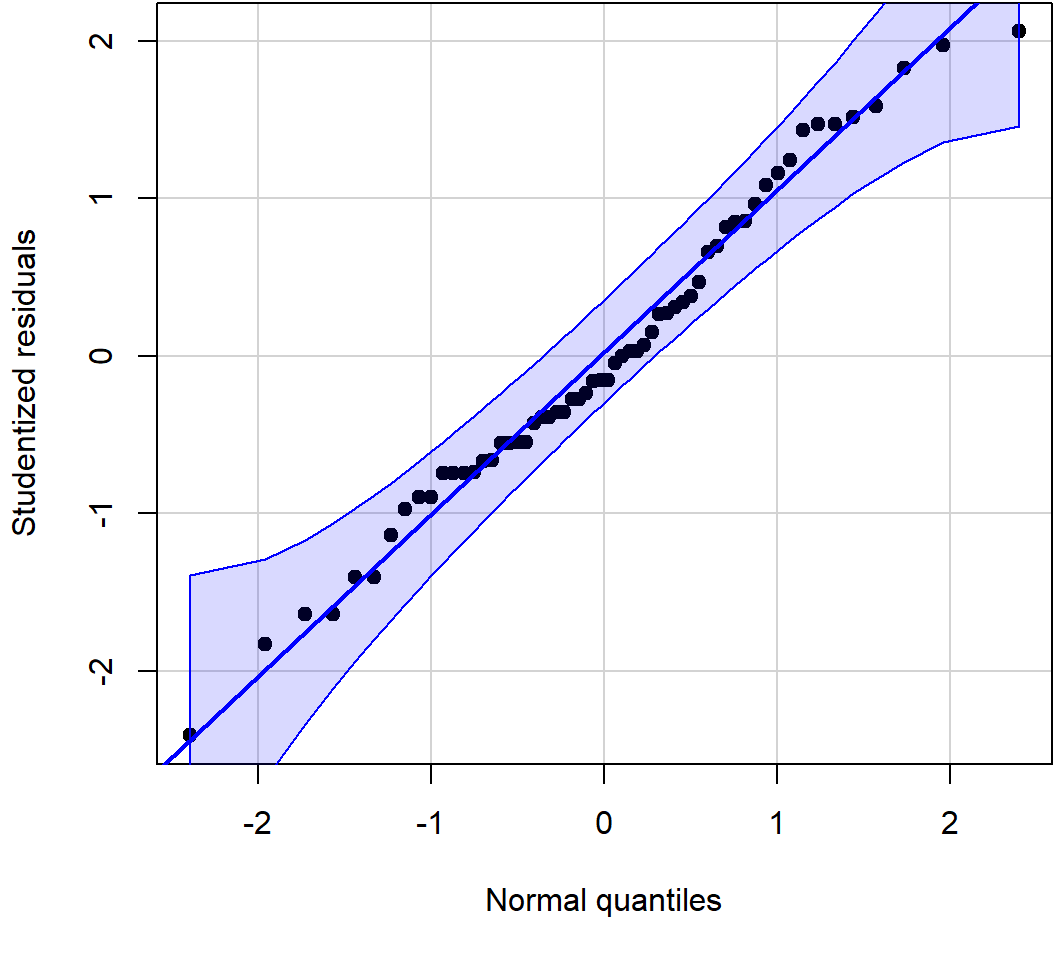
\includegraphics{Tutorials_files/figure-latex/fig-1.pdf}
\caption{\label{fig:fig}Normal quantile-quantile plot of the studentized residuals showed no notable deviation from normality.}
\end{figure}

\emph{If} you include any supplementary material, you should refer to it in the main text.

\begin{center}\rule{0.5\linewidth}{0.5pt}\end{center}

\hypertarget{chi-squared-test}{%
\chapter{Chi-Squared Test}\label{chi-squared-test}}

A test for comparing observed to expected frequencies

\begin{center}\rule{0.5\linewidth}{0.5pt}\end{center}

Summary

\begin{enumerate}
\def\labelenumi{\arabic{enumi}.}
\tightlist
\item
  \href{https://youtu.be/BGUqZc-Pb8w}{Read the data into R };
\item
  Visualize the data;
\item
  Choose an appropriate \href{https://youtu.be/PDl7mhpY4PI}{\(\chi^2\)-test };
\item
  Report a conclusion;
\item
  Incorporating this in scientific literature.
\end{enumerate}

You can download the tutorial \href{files/tutorial_chi-squared-test.Rmd}{here} and the required data set \href{data/binary-data.csv}{here}.

\hypertarget{read-the-data-into-r}{%
\section{Read the Data into R}\label{read-the-data-into-r}}

Chi-squared tests usually involve a limited number of variables (otherwise you should probably use a binomial GLM instead). We can therefore just enter the data manually:

\begin{Shaded}
\begin{Highlighting}[]
\CommentTok{\# Example 1: A vector of observed frequencies per category}
\NormalTok{Observed }\OtherTok{\textless{}{-}} \FunctionTok{c}\NormalTok{(}\AttributeTok{rose =} \DecValTok{33}\NormalTok{, }\AttributeTok{tulip =} \DecValTok{6}\NormalTok{, }\AttributeTok{dandelion =} \DecValTok{11}\NormalTok{)}

\CommentTok{\# Example 2: A contingency table}
\NormalTok{ConTable }\OtherTok{\textless{}{-}} \FunctionTok{data.frame}\NormalTok{(}
  \AttributeTok{men   =} \FunctionTok{c}\NormalTok{(}\DecValTok{41}\NormalTok{, }\DecValTok{68}\NormalTok{),}
  \AttributeTok{women =} \FunctionTok{c}\NormalTok{(}\DecValTok{33}\NormalTok{, }\DecValTok{82}\NormalTok{) }
\NormalTok{)}
\FunctionTok{rownames}\NormalTok{(ConTable) }\OtherTok{\textless{}{-}} \FunctionTok{c}\NormalTok{(}\StringTok{"non{-}smoking"}\NormalTok{, }\StringTok{"smoking"}\NormalTok{)}
\end{Highlighting}
\end{Shaded}

I have a tidy data file

\begin{table}

\caption{\label{tab:unnamed-chunk-24}First 5 rows of a tidy data set with only categorical data.}
\centering
\fontsize{11}{13}\selectfont
\begin{tabular}[t]{c|c}
\hline
smoking & sex\\
\hline
FALSE & man\\
\hline
FALSE & man\\
\hline
FALSE & man\\
\hline
FALSE & man\\
\hline
FALSE & man\\
\hline
... & ...\\
\hline
\end{tabular}
\end{table}

If you have data in tidy format, you can easily generate a contingency table with the function \texttt{table}:

Details

\begin{itemize}
\tightlist
\item
  Save the data in a folder;
\item
  Open RStudio and create a new R markdown file; (\textbf{File} \textgreater{} \textbf{New File} \textgreater{} \textbf{R Markdown})
\item
  Save your R markdown file to the same location as the data;
\item
  Set working directory to source file location. (\textbf{Session} \textgreater{} \textbf{Set Working Directory} \textgreater{} \textbf{To Source File Location})
\end{itemize}

\begin{Shaded}
\begin{Highlighting}[]
\CommentTok{\# Read the data}
\NormalTok{DF }\OtherTok{\textless{}{-}} \FunctionTok{read.csv}\NormalTok{(}\StringTok{"binary{-}data.csv"}\NormalTok{)}

\CommentTok{\# Convert tidy data to a contingency table}
\NormalTok{ConTable }\OtherTok{\textless{}{-}} \FunctionTok{table}\NormalTok{(DF)}

\CommentTok{\# Print the object to confirm it worked}
\FunctionTok{print}\NormalTok{(ConTable)}
\end{Highlighting}
\end{Shaded}

\begin{verbatim}
##        sex
## smoking man woman
##   FALSE  41    33
##   TRUE   68    82
\end{verbatim}

Common mistakes

\begin{itemize}
\tightlist
\item
  Remember to include the file extension (e.g., ``binary-data\textbf{.csv}'') when typing the file name.
\item
  You cannot read Excel files (.xls, .xlsx) with this function. Instead, follow the guide \protect\hyperlink{read}{here}, or save your data as CSV.
\item
  Don't open the CSV file with Excel. You don't need Excel or Google Sheets or any other program besides R and RStudio. If you have saved your data as CSV, you can close Excel.
\end{itemize}

\hypertarget{vis-chi}{%
\section{Visualize the Data}\label{vis-chi}}

If your data can be summarized as a \(2 \times 2\) contingency table, I recommend just including it as is:

\begin{table}

\caption{\label{tab:unnamed-chunk-27}Contingency table of smoking and sex.}
\centering
\begin{tabular}[t]{>{}l|r|r}
\hline
  & men & women\\
\hline
\textbf{non-smoking} & 41 & 33\\
\hline
\textbf{smoking} & 68 & 82\\
\hline
\end{tabular}
\end{table}

Plotting categorical data

There are several options for plotting categorical data. In summary:

\begin{itemize}
\tightlist
\item
  Marginal bar charts cannot show combinations of variables;
\item
  Grouped bar charts \emph{can} show combinations of variables;
\item
  A mosaic plot is an alternative to a grouped bar chart.
\end{itemize}

Marginal bar chart

A marginal bar chart shows you the totals of one variable, summed over all other variables. They are what you would find at the \emph{margins} of a contingency table if you were to include the totals:

\begin{Shaded}
\begin{Highlighting}[]
\FunctionTok{barplot}\NormalTok{(}\FunctionTok{rowSums}\NormalTok{(ConTable))}
\FunctionTok{barplot}\NormalTok{(}\FunctionTok{colSums}\NormalTok{(ConTable))}
\end{Highlighting}
\end{Shaded}

\begin{figure}
\centering
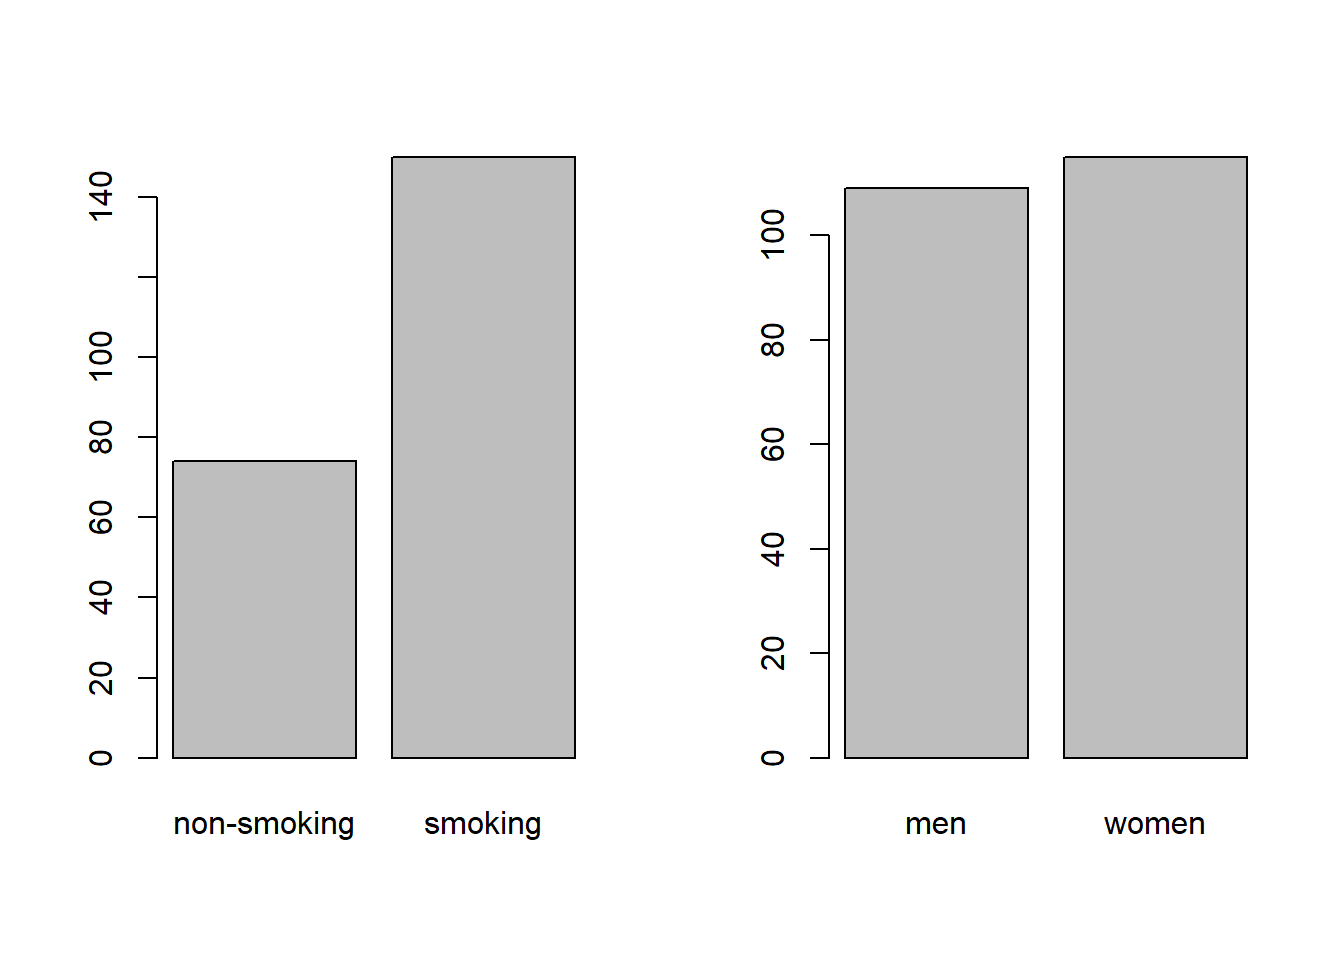
\includegraphics{Tutorials_files/figure-latex/unnamed-chunk-29-1.pdf}
\caption{\label{fig:unnamed-chunk-29}Marginal bar chart of smoking (A) and sex (B).}
\end{figure}

While this provides easy insight into the marginal distribution of smoking (A) and sex (B), it cannot show you combinations of the two, and is therefore not always informative.

Of course, if your data only contains counts of a single variable, then a marginal bar chart is appropriate:

\begin{Shaded}
\begin{Highlighting}[]
\FunctionTok{barplot}\NormalTok{(Observed, }\AttributeTok{col =} \FunctionTok{c}\NormalTok{(}\StringTok{"red"}\NormalTok{, }\StringTok{"orange"}\NormalTok{, }\StringTok{"yellow"}\NormalTok{))}
\end{Highlighting}
\end{Shaded}

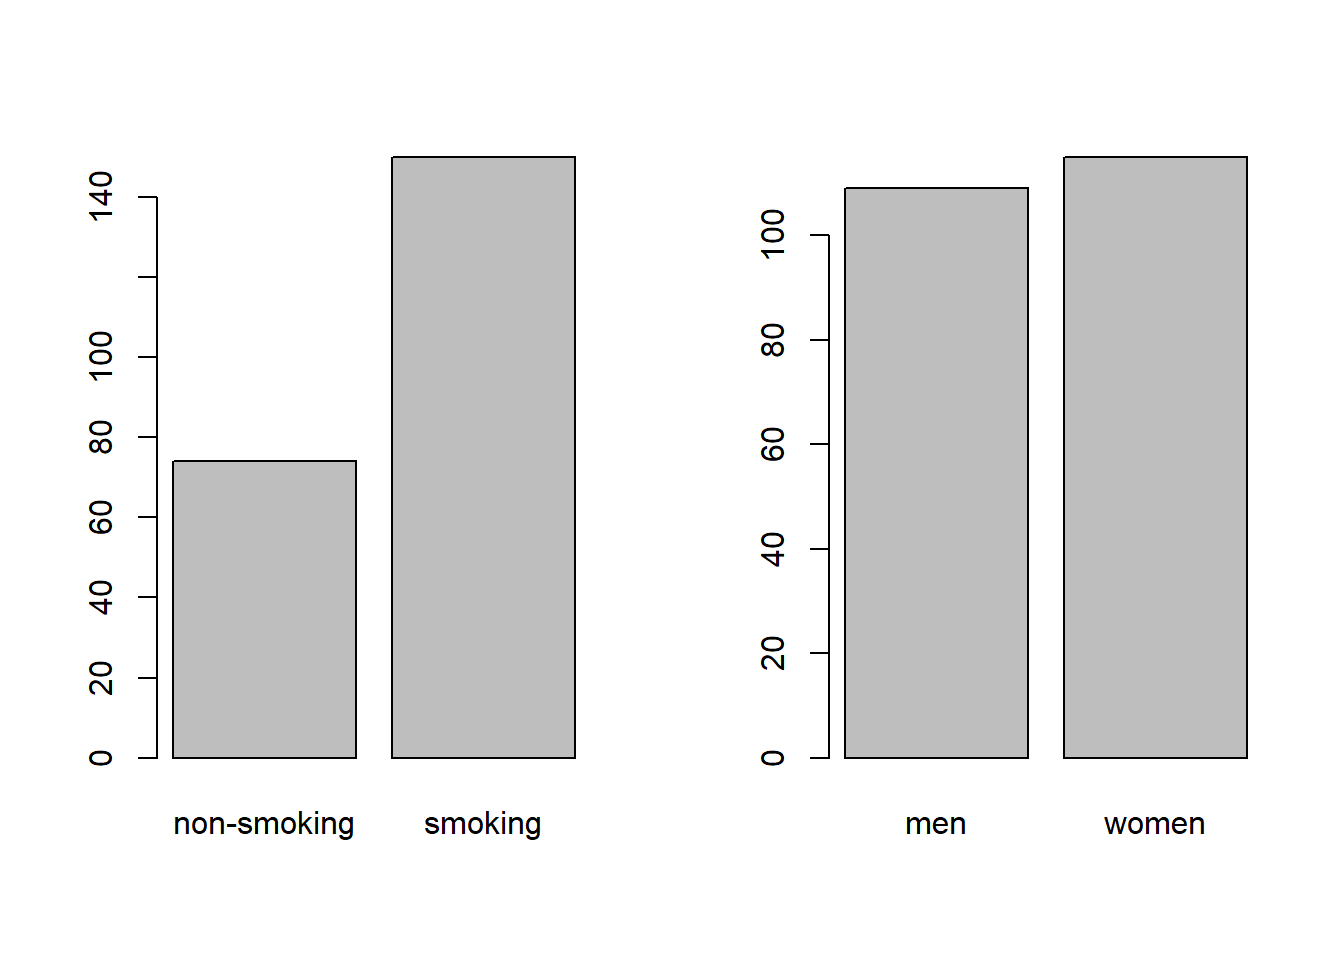
\includegraphics{Tutorials_files/figure-latex/unnamed-chunk-30-1.pdf}

Grouped bar chart

A grouped bar chart shows the frequencies of one variable, split by another:

\begin{Shaded}
\begin{Highlighting}[]
\FunctionTok{barplot}\NormalTok{(}\FunctionTok{as.matrix}\NormalTok{(ConTable), }\AttributeTok{beside =} \ConstantTok{TRUE}\NormalTok{, }\AttributeTok{xlim =} \FunctionTok{c}\NormalTok{(}\DecValTok{1}\NormalTok{, }\DecValTok{8}\NormalTok{), }\AttributeTok{col =} \DecValTok{3}\SpecialCharTok{:}\DecValTok{4}\NormalTok{)}
\FunctionTok{legend}\NormalTok{(}\StringTok{"topright"}\NormalTok{, }\AttributeTok{legend =} \FunctionTok{rownames}\NormalTok{(ConTable), }\AttributeTok{pch =} \DecValTok{15}\NormalTok{, }\AttributeTok{col =} \DecValTok{3}\SpecialCharTok{:}\DecValTok{4}\NormalTok{)}
\end{Highlighting}
\end{Shaded}

\begin{figure}
\centering
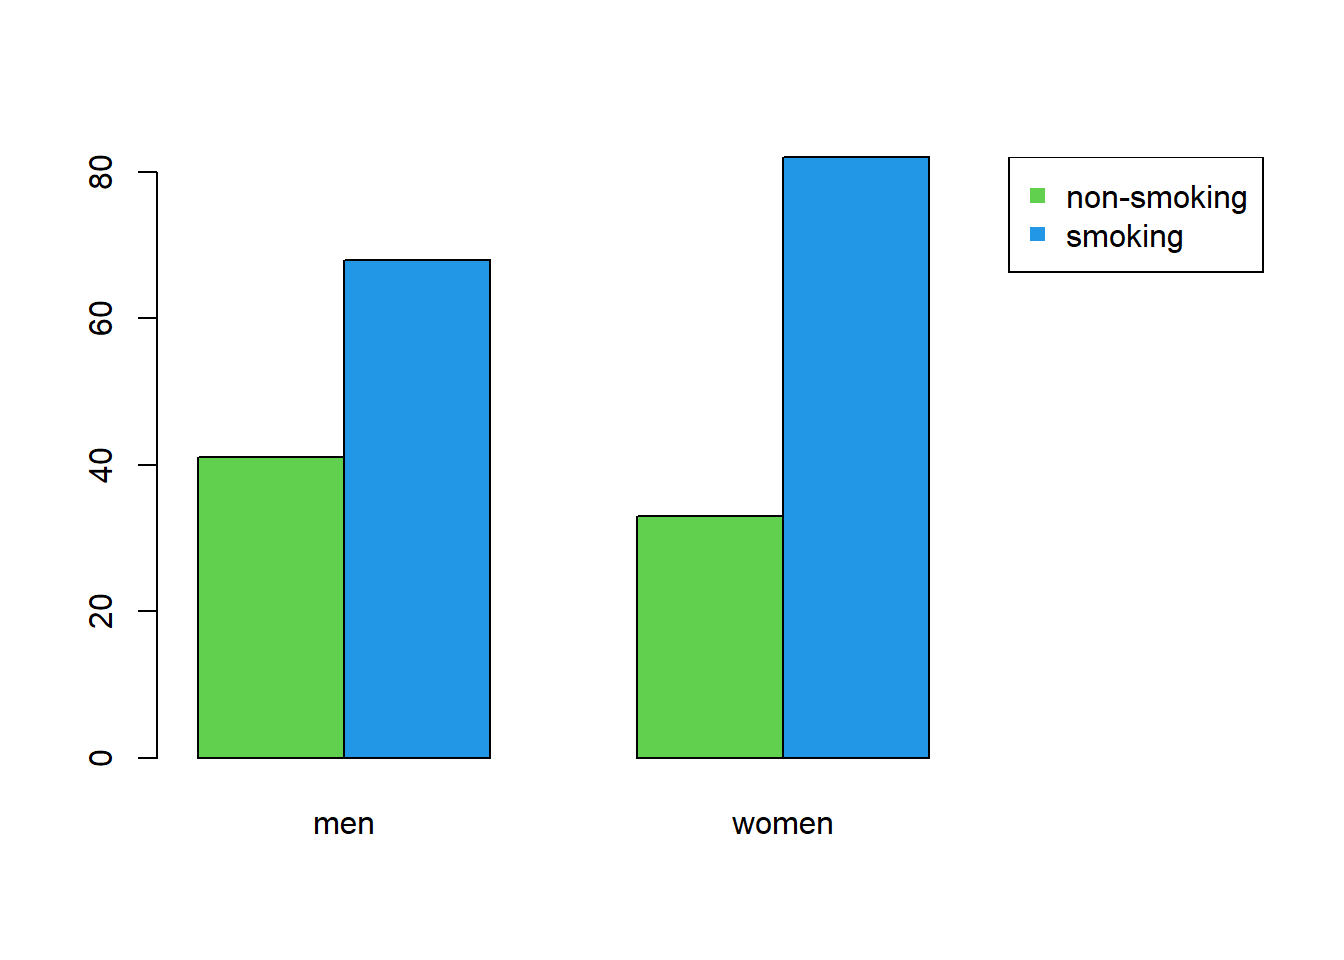
\includegraphics{Tutorials_files/figure-latex/unnamed-chunk-31-1.pdf}
\caption{\label{fig:unnamed-chunk-31}Grouped bar chart of smoking and sex.}
\end{figure}

A grouped bar chart has the advantage of showing not the marginals, but combinations of smoking and sex in a single figure.

Improving your plot

Some basic adjustments that improve bar charts:

\begin{itemize}
\tightlist
\item
  Add an informative caption;
\item
  Keep the numbers on the axes horizontal where possible;
\item
  Remove unnecessary plot elements, like boxes around the bars;
\item
  \textbf{Never} start a bar chart at a different height than zero. This is fine for just about every other type of plot, but in a bar chart, it warps the perceived difference in relative height.
\end{itemize}

The changes to the code I made below can all be found in the help pages \texttt{?barplot} and \texttt{?par}. I am also a big fan of the \texttt{eaxis} function from the package \texttt{sfsmisc}. The caption is added as a chunk option (i.e., \texttt{\textasciigrave{}\textasciigrave{}\textasciigrave{}\{r,\ fig.cap\ =\ "..."\}}).

\begin{Shaded}
\begin{Highlighting}[]
\CommentTok{\# Change the margins (bottom, left, top, right)}
\FunctionTok{par}\NormalTok{(}\AttributeTok{mar =} \FunctionTok{c}\NormalTok{(}\FloatTok{2.5}\NormalTok{, }\DecValTok{4}\NormalTok{, }\DecValTok{0}\NormalTok{, }\DecValTok{0}\NormalTok{) }\SpecialCharTok{+} \FloatTok{0.1}\NormalTok{)}

\CommentTok{\# barplot() expects a matrix. We will need this object several times:}
\NormalTok{M }\OtherTok{\textless{}{-}} \FunctionTok{as.matrix}\NormalTok{(ConTable)}

\CommentTok{\# Color{-}blind friendly colors picked from: https://colorbrewer2.org/}
\NormalTok{cols }\OtherTok{\textless{}{-}} \FunctionTok{c}\NormalTok{(}\StringTok{"\#1f78b4"}\NormalTok{, }\StringTok{"\#b2df8a"}\NormalTok{)}

\CommentTok{\# Create the coordinate system}
\FunctionTok{barplot}\NormalTok{(M, }\AttributeTok{beside =} \ConstantTok{TRUE}\NormalTok{, }\AttributeTok{xlim =} \FunctionTok{c}\NormalTok{(}\DecValTok{0}\NormalTok{, }\DecValTok{9}\NormalTok{), }\AttributeTok{ylim =} \FunctionTok{c}\NormalTok{(}\DecValTok{0}\NormalTok{, }\DecValTok{90}\NormalTok{), }\AttributeTok{axes =} \ConstantTok{FALSE}\NormalTok{, }
        \AttributeTok{col =}\NormalTok{ cols, }\AttributeTok{border =} \ConstantTok{NA}\NormalTok{, }\AttributeTok{xaxs =} \StringTok{"i"}\NormalTok{, }\AttributeTok{ylab =} \StringTok{"Frequency"}\NormalTok{)}

\CommentTok{\# Add y{-}axis}
\FunctionTok{eaxis}\NormalTok{(}\DecValTok{2}\NormalTok{)}

\CommentTok{\# Add a lightgrey background}
\FunctionTok{polygon}\NormalTok{(}\AttributeTok{x =} \FunctionTok{c}\NormalTok{(}\SpecialCharTok{{-}}\DecValTok{1}\NormalTok{, }\DecValTok{7}\NormalTok{, }\DecValTok{7}\NormalTok{, }\SpecialCharTok{{-}}\DecValTok{1}\NormalTok{, }\SpecialCharTok{{-}}\DecValTok{1}\NormalTok{), }\AttributeTok{y =} \FunctionTok{c}\NormalTok{(}\DecValTok{0}\NormalTok{, }\DecValTok{0}\NormalTok{, }\DecValTok{100}\NormalTok{, }\DecValTok{100}\NormalTok{, }\DecValTok{0}\NormalTok{), }
        \AttributeTok{col =} \StringTok{"grey95"}\NormalTok{, }\AttributeTok{border =} \ConstantTok{NA}\NormalTok{)}

\CommentTok{\# Add a simple grid}
\FunctionTok{abline}\NormalTok{(}\AttributeTok{h =} \FunctionTok{seq}\NormalTok{(}\DecValTok{0}\NormalTok{, }\DecValTok{100}\NormalTok{, }\DecValTok{10}\NormalTok{), }\AttributeTok{col =} \StringTok{"white"}\NormalTok{, }\AttributeTok{lwd =} \DecValTok{1}\NormalTok{)}
\FunctionTok{abline}\NormalTok{(}\AttributeTok{h =} \FunctionTok{seq}\NormalTok{(}\DecValTok{0}\NormalTok{, }\DecValTok{100}\NormalTok{, }\DecValTok{20}\NormalTok{), }\AttributeTok{col =} \StringTok{"white"}\NormalTok{, }\AttributeTok{lwd =} \FloatTok{1.5}\NormalTok{)}

\CommentTok{\# Redraw the barplot on top}
\FunctionTok{barplot}\NormalTok{(M, }\AttributeTok{beside =} \ConstantTok{TRUE}\NormalTok{, }\AttributeTok{xlim =} \FunctionTok{c}\NormalTok{(}\DecValTok{1}\NormalTok{, }\DecValTok{8}\NormalTok{), }\AttributeTok{axes =} \ConstantTok{FALSE}\NormalTok{, }\AttributeTok{add =} \ConstantTok{TRUE}\NormalTok{,}
        \AttributeTok{col =}\NormalTok{ cols, }\AttributeTok{border =} \ConstantTok{NA}\NormalTok{)}

\CommentTok{\# Create a legend}
\FunctionTok{legend}\NormalTok{(}\StringTok{"topright"}\NormalTok{, }\AttributeTok{legend =} \FunctionTok{rownames}\NormalTok{(M), }\AttributeTok{pch =} \DecValTok{15}\NormalTok{, }\AttributeTok{col =}\NormalTok{ cols, }\AttributeTok{bty =} \StringTok{"n"}\NormalTok{)}

\CommentTok{\# Restore the default margins for subsequent plots}
\FunctionTok{par}\NormalTok{(}\AttributeTok{mar =} \FunctionTok{c}\NormalTok{(}\DecValTok{5}\NormalTok{, }\DecValTok{4}\NormalTok{, }\DecValTok{4}\NormalTok{, }\DecValTok{3}\NormalTok{) }\SpecialCharTok{+} \FloatTok{0.1}\NormalTok{)}
\end{Highlighting}
\end{Shaded}

\begin{figure}
\centering
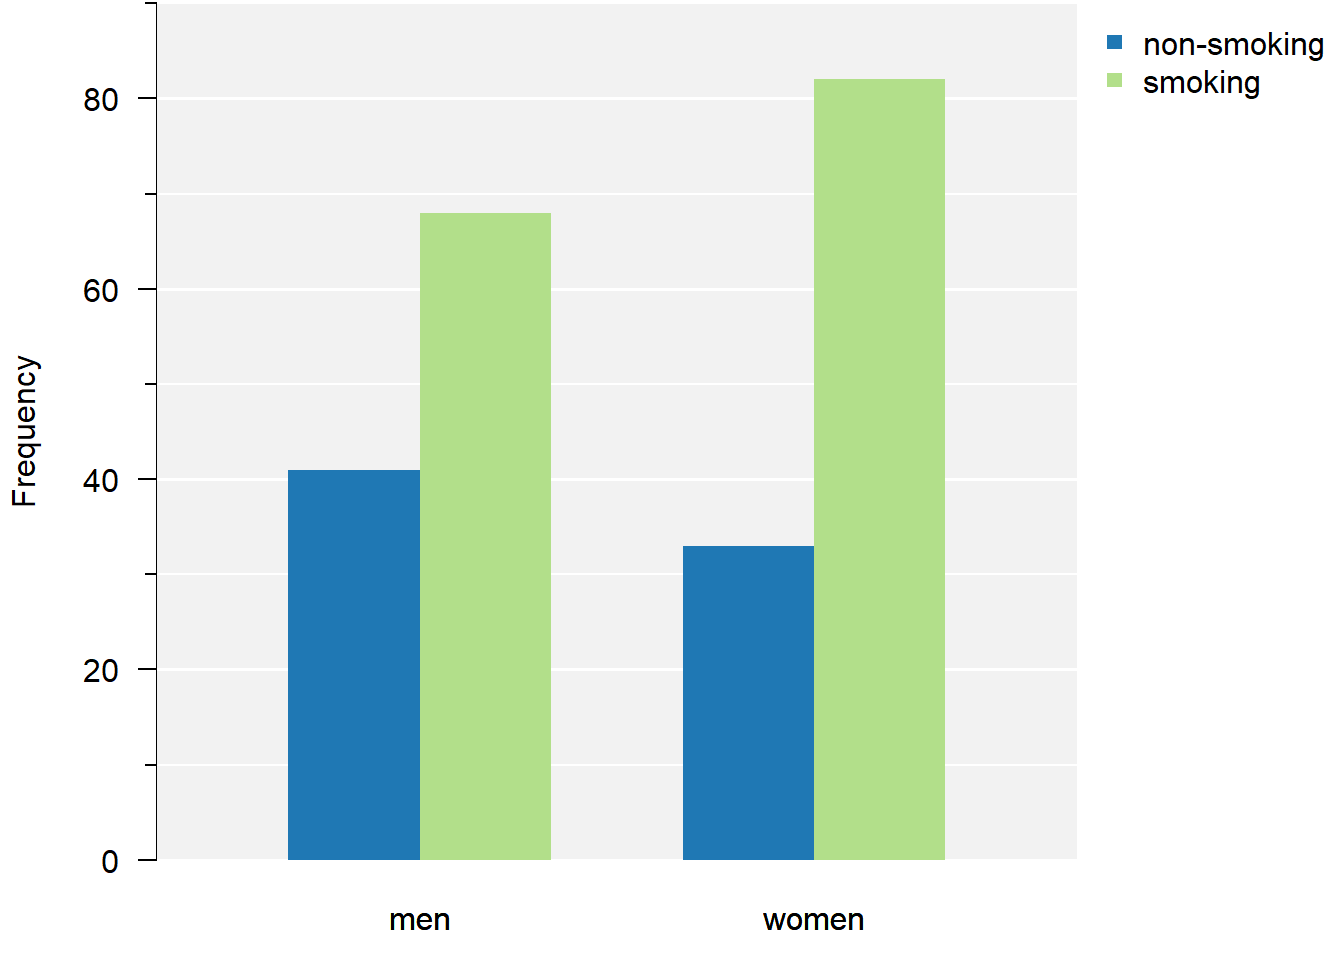
\includegraphics{Tutorials_files/figure-latex/unnamed-chunk-33-1.pdf}
\caption{\label{fig:unnamed-chunk-33}Grouped bar chart of smoking and sex.}
\end{figure}

From the plot we can conclude there are more smokers than non-smokers. Smoking appears slightly more common in females.

Mosaic plot

A mosaic plot is \emph{similar} to a stacked bar chart (groups pasted on top of each other). However, in a mosaic plot, both the height \emph{and} the width of the bars is proportional to the frequency of that group:

\begin{Shaded}
\begin{Highlighting}[]
\FunctionTok{mosaicplot}\NormalTok{(ConTable, }\AttributeTok{main =} \StringTok{""}\NormalTok{, }\AttributeTok{col =} \DecValTok{3}\SpecialCharTok{:}\DecValTok{4}\NormalTok{)}
\end{Highlighting}
\end{Shaded}

\begin{figure}
\centering
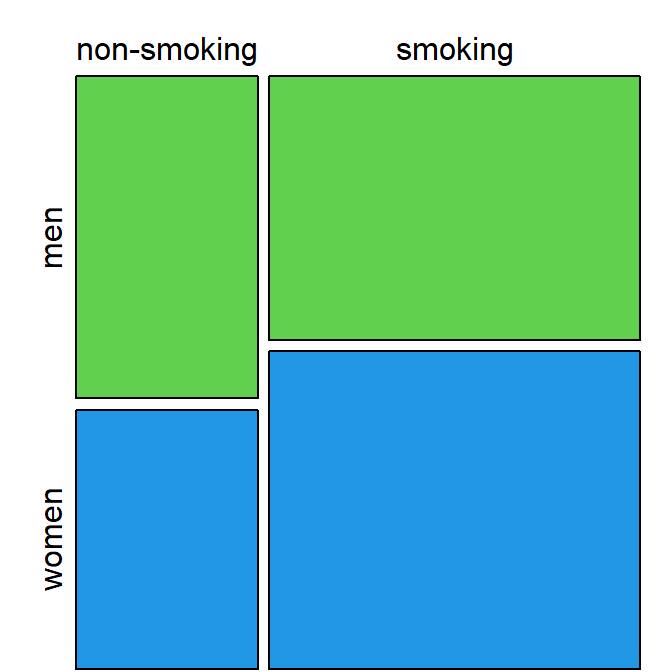
\includegraphics{Tutorials_files/figure-latex/unnamed-chunk-35-1.pdf}
\caption{\label{fig:unnamed-chunk-35}Mosaic plot of smoking and sex shows smoking is relatively, slightly more common in women.}
\end{figure}

Mosaic plots are not very commonly used, but can provide an alternative to bar charts to summarize categorical data effectively, especially with an appropriate color scheme to distinguish between categories.

\hypertarget{conduct-a-chi-squared-test}{%
\section{Conduct a Chi-Squared Test}\label{conduct-a-chi-squared-test}}

If you have a single set of observed values

To compare a single set of observed values to their expected proportions:

\begin{Shaded}
\begin{Highlighting}[]
\CommentTok{\# Proportions in which the flowers were planted}
\NormalTok{expected }\OtherTok{\textless{}{-}} \FunctionTok{c}\NormalTok{(}\DecValTok{1}\SpecialCharTok{/}\DecValTok{2}\NormalTok{, }\DecValTok{1}\SpecialCharTok{/}\DecValTok{4}\NormalTok{, }\DecValTok{1}\SpecialCharTok{/}\DecValTok{4}\NormalTok{)}

\CommentTok{\# Did the flowers sprout in a different ratio than I planted them?}
\FunctionTok{chisq.test}\NormalTok{(Observed, }\AttributeTok{p =}\NormalTok{ expected)}
\end{Highlighting}
\end{Shaded}

\begin{verbatim}
## 
##  Chi-squared test for given probabilities
## 
## data:  Observed
## X-squared = 6.12, df = 2, p-value = 0.04689
\end{verbatim}

If you have a contingency table

To conduct a \(\chi^2\)-test for independence:

\begin{Shaded}
\begin{Highlighting}[]
\FunctionTok{chisq.test}\NormalTok{(ConTable)}
\end{Highlighting}
\end{Shaded}

\begin{verbatim}
## 
##  Pearson's Chi-squared test with Yates' continuity correction
## 
## data:  ConTable
## X-squared = 1.6293, df = 1, p-value = 0.2018
\end{verbatim}

I received a warning

If you receive the following warning:

\begin{verbatim}
Warning message:
In chisq.test(Observed, p = expected) :
  Chi-squared approximation may be incorrect
\end{verbatim}

That means at least one of the expected values is less than 5. The solution is to use Monte Carlo simulation to estimate the \(p\)-value (for a vector of observed frequencies) use an exact test (for contingency tables):

\begin{Shaded}
\begin{Highlighting}[]
\CommentTok{\# Monte Carlo (for a vector of observed frequencies)}
\FunctionTok{chisq.test}\NormalTok{(Observed, }\AttributeTok{simulate.p.value =} \ConstantTok{TRUE}\NormalTok{)}

\CommentTok{\# Exact test (for contingency tables)}
\FunctionTok{fisher.test}\NormalTok{(ConTable)}
\end{Highlighting}
\end{Shaded}

\hypertarget{results-chi}{%
\section{Correctly Phrase the Results}\label{results-chi}}

For a \textbf{vector of observed frequencies}:

If the \(p\)-value is \textbf{less} than the chosen level of significance

\emph{(This is the case in the flower example.)}

Examples of precise language:

\begin{itemize}
\tightlist
\item
  Flowers species were counted in a ratio significantly different from the \(2:1:1\) ratio in which they were planted (\(\chi^2 = 24.8\), \(p = 4.20 \cdot 10^{-6}\));
\item
  We observed significantly different proportions of flower species than expected (\(\chi^2 = 24.8\), \(p = 4.20 \cdot 10^{-6}\)).
\end{itemize}

Examples of incorrect, incomplete, or imprecise language:

\begin{itemize}
\tightlist
\item
  The alternative hypothesis was true // The null-hypothesis was false;
\item
  The difference was significant (\(p < 0.05\));
\item
  Flowers species sprout in a different ratio than the ratio in which they are planted.
\end{itemize}

Why paste tense?

The results of a single experiment, no matter how convincing, can never prove something to be true. The results \emph{were} observed, and in this one experiment, A \emph{was} better than B.

Use present tense only for statements that have been demonstrated repeatedly, are generally agreed upon, or are easily observable, e.g.:

\begin{itemize}
\tightlist
\item
  Smoking causes cancer;
\item
  Current climate-change is mainly caused by human activities;
\item
  Most people use smartphones nowadays.
\end{itemize}

If the \(p\)-value is \textbf{greater} than the chosen level of significance

Examples of precise language:

\begin{itemize}
\tightlist
\item
  Counts of flowers species did not differ significantly from the \(2:1:1\) ratio in which they were planted (\(\chi^2 = \dots\), \(p = \dots\));
\item
  There is insufficient evidence to conclude a difference from a \(2:1:1\) ratio (\(\chi^2 = \dots\), \(p = \dots\));
\item
  There was a trend towards more rose and fewer tulips than expected under a \(2:1:1\) ratio, but this difference was not significant (\(\chi^2 = \dots\), \(p = \dots\)).
\end{itemize}

Examples of incorrect, incomplete, or imprecise language:

\begin{itemize}
\tightlist
\item
  Planting and sprouting ratios were equal // The \(2:1:1\) ratio was correct;
\item
  There was no difference (\(p < 0.05\));
\item
  We accept the null-hypothesis.
\end{itemize}

Why can't I say I \emph{accepted} the null-hypothesis?

This is imprecise language because it distorts the order of null-hypothesis significance testing. Every tests \emph{starts} with pretending the null-hypothesis is true, and then considering how rare a result this would be. You did not accept the null-hypothesis \emph{because} of the \(p\)-value, but rather, you started by taking on the null-hypothesis to even compute that \(p\)-value.

For \textbf{contingency tables}:

If the \(p\)-value is \textbf{less} than the chosen level of significance

Examples of precise language:

\begin{itemize}
\tightlist
\item
  Smoking behavior differed significantly by sex (\(\chi^2 = \dots\), \(p = \dots\));
\item
  Females were proportionally significantly more likely to be smokers (\(\chi^2 = \dots\), \(p = \dots\)).
\item
  Smoking behavior and sex were significantly dependent (\(\chi^2 = \dots\), \(p = \dots\)).
\end{itemize}

Examples of incorrect, incomplete, or imprecise language:

\begin{itemize}
\tightlist
\item
  The alternative hypothesis was true // The null-hypothesis was false;
\item
  The difference was significant (\(p < 0.05\));
\item
  Sex and smoking are independent of each other.
\end{itemize}

Why paste tense?

The results of a single experiment, no matter how convincing, can never prove something to be true. The results \emph{were} observed, and in this one experiment, A \emph{was} better than B.

Use present tense only for statements that have been demonstrated repeatedly, are generally agreed upon, or are easily observable, e.g.:

\begin{itemize}
\tightlist
\item
  Smoking causes cancer;
\item
  Current climate-change is mainly caused by human activities;
\item
  Most people use smartphones nowadays.
\end{itemize}

If the \(p\)-value is \textbf{greater} than the chosen level of significance

Examples of precise language:

\begin{itemize}
\tightlist
\item
  Smoking behavior did not differ significantly by sex (\(\chi^2 = \dots\), \(p = \dots\));
\item
  There is insufficient evidence to conclude a difference in smoking behavior between men and women (\(\chi^2 = \dots\), \(p = \dots\));
\item
  Smoking behavior and sex did not depend significantly on each other (\(\chi^2\), \(p\)).
\end{itemize}

Examples of incorrect, incomplete, or imprecise language:

\begin{itemize}
\tightlist
\item
  Smoking behavior was equal for men and women // Sex and smoking were independent;
\item
  There was no difference (\(p < 0.05\));
\item
  We accept the null-hypothesis.
\end{itemize}

Why can't I say I \emph{accepted} the null-hypothesis?

This is imprecise language because it distorts the order of null-hypothesis significance testing. Every tests \emph{starts} with pretending the null-hypothesis is true, and then considering how rare a result this would be. You did not accept the null-hypothesis \emph{because} of the \(p\)-value, but rather, you started by taking on the null-hypothesis to even compute that \(p\)-value.

\hypertarget{incorporating-this-in-a-paper-1}{%
\section{Incorporating This in a Paper}\label{incorporating-this-in-a-paper-1}}

Here you can find examples of how to justify the methods used, explain the results found and write a discussion. This is meant to show you what belongs where, and what level of detail is common in scientific literature.

Remember to use your own words---\textbf{paraphrase to avoid plagiarism}.

Methods

\emph{(In this section, you should describe the data collection and analysis to an extent that a fellow expert could reproduce your study.)}

All 226 employees at Example company were inquired about their sex and smoking behavior in November 2022. A total of \(n = 224\) employees responded.

All statistical analyses were conducted in R, version 4.2.1, using the RStudio interface.\citep{R, RStudio} Observed and expected frequencies were compared with a Pearson's chi-squared test.

Note:

\begin{itemize}
\tightlist
\item
  Check your R version number with \texttt{version};
\item
  Justify the type of test used; \emph{(If you use a \(\chi^2\)-test, all expected (not observed) counts should be greater than 5.)}
\item
  You should cite any packages used to perform analyses, generate tables or figures that made it into the paper, e.g.;

  \begin{itemize}
  \tightlist
  \item
    Figures were created with the \texttt{ggplot2} package.\citep{ggplot2} \emph{(Not the case in the tutorial.)}
  \end{itemize}
\item
  You should \emph{not} cite packages used only internally, e.g.:

  \begin{itemize}
  \tightlist
  \item
    We used \texttt{readxl} to enter the data in R.\citep{readxl}
  \end{itemize}
\item
  It is important to mention adequately how the data was collected. For survey research like that in the example, the respondence rate can have a large influence on the conclusions: What if smoking females are less likely to respond?
\end{itemize}

Results

\emph{(In this section you should mention the results without giving any interpretation yet.)}

For general advice on phrasing, see: \protect\hyperlink{results-chi}{Correctly Phrase the Results}. In this section, you should include your table and/or figure of the data and explain in brief what the outcome of the \(\chi^2\)-test was.

It is very common to see bar charts with significance stars, but the interpretation of these stars is not consistent and you should mention the actual, non-discretized \(p\)-value at least somewhere in the results.

Discussion

\emph{(In this section, you should not mention results, but the conclusions based on those results.)}

For a \textbf{vector of observed frequencies}:

If the test was significant \textbf{and} the difference large enough to be biologically relevant

\emph{(This is the case in the flower example.)}

\begin{itemize}
\tightlist
\item
  Roses appear to sprout more often, and tulips less often than dandelions, though more replicates of the experiment are necessary for a conclusive answer;
\item
  Differences in seed resilience of roses, tulips and dandelions may cause them to sprout disproportional to their planting ratios.
\item
  \emph{(Overclaiming)} Roses are better at sprouting than tulips or dandelions.
\item
  \emph{(Overgeneralizing)} Thorned flowers appear to sprout more often than flowers without thorns.
\end{itemize}

If the test was insignificant \textbf{or} the difference too small to be biologically relevant:

\begin{itemize}
\tightlist
\item
  \emph{(If the study was sufficiently powerful)} Despite a fairly large sample size, we were unable to demonstrate a difference in planting and sprouting ratios, suggesting these species are equally likely to sprout when planted.
\item
  \emph{(If the study was underpowered)} We were unable to demonstrate a difference in planting and sprouting ratios, though a multiple replications of the experiment in different fields may yield a more conclusive answer.
\item
  \emph{(Appeal to ignorance)} We have demonstrated there is no difference in planting and sprouting ratios.
\end{itemize}

Why can't I conclude there is no difference?

This is an inherent limitation of the \(p\)-value. Under the null-hypothesis, any \(p\)-value is as likely as any other (uniformity). Therefore, even if the \(p\)-value is very large, this cannot be interpreted as evidence \emph{for} the null-hypothesis.

For example, a \(p\)-value of \(0.20\) is just as common a result as \(0.80\) when the null-hypothesis is correct. The \(p\)-value can \emph{only} be used as evidence \emph{against} the null-hypothesis (when it is small).

If you want to perform a test to find out whether the null-hypothesis is correct, what you are looking for is called an \href{https://en.wikipedia.org/wiki/Equivalence_test}{equivalence test}.

Also see: \href{https://stats.stackexchange.com/a/85914/176202}{Why do statisticians say a non-significant result means ``you can't reject the null'' as opposed to accepting the null hypothesis?}

For \textbf{contingency tables}:

If the test was significant \textbf{and} the difference large enough to be biologically relevant

\begin{itemize}
\tightlist
\item
  Women may be more inclined to smoke at work, though more replicates of the experiment at different companies are necessary for a conclusive answer;
\item
  Anti-smoking campaigns at Example company may have been relatively more effective at targeting men, though a longitudinal intervention study could provide a more conclusive answer.
\item
  \emph{(Overclaiming)} Anti-smoking campaigns at Example company have been more successful in targeting men.
\item
  \emph{(Overgeneralizing)} Men are less inclined to smoke at work.
\end{itemize}

If the test was insignificant \textbf{or} the difference too small to be biologically relevant:

\emph{(This is the case in the smoking example.)}

\begin{itemize}
\tightlist
\item
  \emph{(If the study was sufficiently powerful)} Smoking remains prevalent at Example company, irrespective of sex.
\item
  \emph{(If the study was underpowered)} We were unable to demonstrate a difference in smoking ratios of men and women at Example company.
\item
  \emph{(Appeal to ignorance)} We have demonstrated smoking and sex are independent at Example company.
\end{itemize}

Why can't I conclude there is no difference?

This is an inherent limitation of the \(p\)-value. Under the null-hypothesis, any \(p\)-value is as likely as any other (uniformity). Therefore, even if the \(p\)-value is very large, this cannot be interpreted as evidence \emph{for} the null-hypothesis.

For example, a \(p\)-value of \(0.20\) is just as common a result as \(0.80\) when the null-hypothesis is correct. The \(p\)-value can \emph{only} be used as evidence \emph{against} the null-hypothesis (when it is small).

If you want to perform a test to find out whether the null-hypothesis is correct, what you are looking for is called an \href{https://en.wikipedia.org/wiki/Equivalence_test}{equivalence test}.

Also see: \href{https://stats.stackexchange.com/a/85914/176202}{Why do statisticians say a non-significant result means ``you can't reject the null'' as opposed to accepting the null hypothesis?}

General note: Counts from a single location, work place, or petri dish are never convincing enough for strong conclusive remarks. It is better to have multiple replicates of the whole experiment (fields, companies, petri dishes) and analyze the results with, for instance, a binomial GLM.

Generating citations

Any packages used in analysis should be cited in the methods section. The citations used here can be easily obtained as follows (note that this requires the packages to be installed):

\begin{Shaded}
\begin{Highlighting}[]
\FunctionTok{citation}\NormalTok{()          }\CommentTok{\# Use this to cite R}
\FunctionTok{RStudio.Version}\NormalTok{()   }\CommentTok{\# Use this to cite RStudio}
\FunctionTok{citation}\NormalTok{(}\StringTok{"ggplot2"}\NormalTok{) }\CommentTok{\# Use this to cite a package (here: ggplot2)}
\end{Highlighting}
\end{Shaded}

You can add these entries to a reference manager (e.g., Zotero), or keep a BibTeX file yourself, as shown \href{https://youtu.be/zuuOYjE8m98}{here}.

\begin{center}\rule{0.5\linewidth}{0.5pt}\end{center}

\hypertarget{anova}{%
\chapter{ANOVA}\label{anova}}

A method test to compare any number of means to see if they differ significantly. Observations are assumed to be \textbf{independent}, deviations from the group means are assumed to follow a \textbf{normal distribution}, and groups are assumed to have \textbf{equal variance}.

\begin{center}\rule{0.5\linewidth}{0.5pt}\end{center}

Summary

\begin{enumerate}
\def\labelenumi{\arabic{enumi}.}
\tightlist
\item
  \href{https://youtu.be/BGUqZc-Pb8w}{Read the data into R };
\item
  Visualize the data;
\item
  Fit an ANOVA:

  \begin{itemize}
  \tightlist
  \item
    Perform visual diagnostics to look for deviations from the assumptions;
  \item
    Perform an omnibus test if the assumptions appear reasonable;
  \item
    Perform a post-hoc test if the omnibus test was significant;
  \end{itemize}
\item
  Report a conclusion;
\item
  Incorporating this in scientific literature.
\end{enumerate}

You can download the tutorial \href{files/tutorial_ANOVA.Rmd}{here} and the required data set \href{data/three-groups.csv}{here}.

\hypertarget{read-ANOVA}{%
\section{Read the Data into R}\label{read-ANOVA}}

I recommend saving data as \href{https://youtu.be/BGUqZc-Pb8w}{comma-separated values (CSV)}. If you prefer reading data directly from Excel, have a look \protect\hyperlink{Excel}{here}.

Details

\begin{itemize}
\tightlist
\item
  Save the data in a folder;
\item
  Open RStudio and create a new R markdown file; (\textbf{File} \textgreater{} \textbf{New File} \textgreater{} \textbf{R Markdown})
\item
  Save your R markdown file to the same location as the data;
\item
  Set working directory to source file location. (\textbf{Session} \textgreater{} \textbf{Set Working Directory} \textgreater{} \textbf{To Source File Location})
\end{itemize}

\begin{Shaded}
\begin{Highlighting}[]
\NormalTok{DF }\OtherTok{\textless{}{-}} \FunctionTok{read.csv}\NormalTok{(}\StringTok{"three{-}groups.csv"}\NormalTok{)}
\end{Highlighting}
\end{Shaded}

Did that work? There are several ways to check:

\begin{Shaded}
\begin{Highlighting}[]
\FunctionTok{str}\NormalTok{(DF)}
\FunctionTok{summary}\NormalTok{(DF)}
\FunctionTok{head}\NormalTok{(DF)}
\end{Highlighting}
\end{Shaded}

Explanation of the output

\begin{Shaded}
\begin{Highlighting}[]
\FunctionTok{str}\NormalTok{(DF)}
\end{Highlighting}
\end{Shaded}

\begin{verbatim}
## 'data.frame':    90 obs. of  4 variables:
##  $ SBP      : int  122 119 120 129 127 118 120 124 126 117 ...
##  $ treatment: chr  "thiazide" "thiazide" "thiazide" "thiazide" ...
##  $ age      : int  32 34 36 41 35 38 36 33 39 32 ...
##  $ sex      : chr  "female" "female" "female" "male" ...
\end{verbatim}

This command shows the structure of the data. It is a data frame with \(n = 60\) observations of 4 variables. \texttt{SBP} and age are stored as integers (\texttt{int}), while \texttt{treatment} and \texttt{sex} are stored character vectors (\texttt{chr}).

\begin{verbatim}
##       SBP         treatment              age            sex           
##  Min.   :114.0   Length:90          Min.   :23.00   Length:90         
##  1st Qu.:122.0   Class :character   1st Qu.:32.00   Class :character  
##  Median :127.0   Mode  :character   Median :35.00   Mode  :character  
##  Mean   :131.5                      Mean   :35.69                     
##  3rd Qu.:142.0                      3rd Qu.:38.00                     
##  Max.   :201.0                      Max.   :83.00
\end{verbatim}

\begin{verbatim}
##   SBP treatment age    sex
## 1 122  thiazide  32 female
## 2 119  thiazide  34 female
## 3 120  thiazide  36 female
## 4 129  thiazide  41   male
## 5 127  thiazide  35 female
## 6 118  thiazide  38 female
\end{verbatim}

My output looks different

Then provided you did everything else correctly, the most likely reason is that your data was saved with a version of Excel where a comma is used as a decimal separator (e.g., the Dutch version). The solutions for this is simple, use \texttt{read.csv2}:

\begin{Shaded}
\begin{Highlighting}[]
\NormalTok{DF }\OtherTok{\textless{}{-}} \FunctionTok{read.csv2}\NormalTok{(}\StringTok{"some{-}data{-}with{-}commas.csv"}\NormalTok{)}
\end{Highlighting}
\end{Shaded}

If that doesn't work either, go over the details shown above, or watch the instructions in the \href{https://youtu.be/BGUqZc-Pb8w}{video}.

Common mistakes

\begin{itemize}
\tightlist
\item
  Remember to include the file extension (e.g., ``two-groups\textbf{.csv}'') when typing the file name.
\item
  You cannot read Excel files (.xls, .xlsx) with this function. Instead, follow the guide \protect\hyperlink{read}{here}, or save your data as CSV.
\item
  Don't open the CSV file with Excel. You don't need Excel or Google Sheets or any other program besides R and RStudio. If you have saved your data as CSV, you can close Excel.
\end{itemize}

The next step is to ensure categorical variables are read as factors. This will allow us to use generic functions like \texttt{plot} and \texttt{summary} in a more meaningful way.

Why not just use \texttt{character}?

A character vector is just strings of text, numbers and/or symbols. If you were to produce a \texttt{summary}, this happens:

\begin{Shaded}
\begin{Highlighting}[]
\FunctionTok{summary}\NormalTok{(DF}\SpecialCharTok{$}\NormalTok{treatment)}
\end{Highlighting}
\end{Shaded}

\begin{verbatim}
##    Length     Class      Mode 
##        90 character character
\end{verbatim}

It tells us this object contains 60 values, and it is stored and treated as a string of text.

The generic \texttt{plot} function doesn't even work at all:

\begin{Shaded}
\begin{Highlighting}[]
\FunctionTok{plot}\NormalTok{(SBP }\SpecialCharTok{\textasciitilde{}}\NormalTok{ treatment, DF)}
\end{Highlighting}
\end{Shaded}

\begin{verbatim}
Error in plot.window(...) : need finite 'xlim' values
In addition: Warning messages:
1: In xy.coords(x, y, xlabel, ylabel, log) : NAs introduced by coercion
2: In min(x) : no non-missing arguments to min; returning Inf
3: In max(x) : no non-missing arguments to max; returning -Inf
\end{verbatim}

Now convert the variables to factors and see how that changes the output. \emph{(Run the code below, then run \texttt{summary(DF\$treatment)}, or \texttt{plot(DF\$treatment)} for example.)}

\begin{Shaded}
\begin{Highlighting}[]
\NormalTok{DF}\SpecialCharTok{$}\NormalTok{treatment }\OtherTok{\textless{}{-}} \FunctionTok{factor}\NormalTok{(DF}\SpecialCharTok{$}\NormalTok{treatment)}
\NormalTok{DF}\SpecialCharTok{$}\NormalTok{sex       }\OtherTok{\textless{}{-}} \FunctionTok{factor}\NormalTok{(DF}\SpecialCharTok{$}\NormalTok{sex)}
\end{Highlighting}
\end{Shaded}

\hypertarget{reordering-a-factor}{%
\subsection*{Reordering a Factor}\label{reordering-a-factor}}
\addcontentsline{toc}{subsection}{Reordering a Factor}

While it does not change any of the conclusions, it can help yourself and any readers if you put the groups in a logical order. For sex there is no logical order, but for treatment it would make sense to have the placebo first, as a reference to compare the other groups to.

To check the order of levels in a factor, use \texttt{levels}:

\begin{Shaded}
\begin{Highlighting}[]
\FunctionTok{levels}\NormalTok{(DF}\SpecialCharTok{$}\NormalTok{treatment)}
\end{Highlighting}
\end{Shaded}

\begin{verbatim}
## [1] "CCB"      "placebo"  "thiazide"
\end{verbatim}

My output is \texttt{NULL}

That means you forgot to convert your variable to a factor first:

\begin{Shaded}
\begin{Highlighting}[]
\FunctionTok{levels}\NormalTok{(DF}\SpecialCharTok{$}\NormalTok{treatment)}
\end{Highlighting}
\end{Shaded}

\begin{verbatim}
## NULL
\end{verbatim}

\begin{Shaded}
\begin{Highlighting}[]
\CommentTok{\# Solution}
\NormalTok{DF}\SpecialCharTok{$}\NormalTok{treatment }\OtherTok{\textless{}{-}} \FunctionTok{factor}\NormalTok{(DF}\SpecialCharTok{$}\NormalTok{treatment)}
\FunctionTok{levels}\NormalTok{(DF}\SpecialCharTok{$}\NormalTok{treatment)}
\end{Highlighting}
\end{Shaded}

\begin{verbatim}
## [1] "CCB"      "placebo"  "thiazide"
\end{verbatim}

To change which treatment appears first, use \texttt{relevel}:

\begin{Shaded}
\begin{Highlighting}[]
\NormalTok{DF}\SpecialCharTok{$}\NormalTok{treatment }\OtherTok{\textless{}{-}} \FunctionTok{relevel}\NormalTok{(DF}\SpecialCharTok{$}\NormalTok{treatment, }\StringTok{"placebo"}\NormalTok{)}
\end{Highlighting}
\end{Shaded}

\emph{(Run \texttt{levels(DF\$treatment)} again to see if it worked.)}

Reordering multiple categories at once

If you want to change the order entirely, you can define the order manually as follows:

\begin{Shaded}
\begin{Highlighting}[]
\NormalTok{DF}\SpecialCharTok{$}\NormalTok{treatment }\OtherTok{\textless{}{-}} \FunctionTok{factor}\NormalTok{(DF}\SpecialCharTok{$}\NormalTok{treatment, }\AttributeTok{levels =} \FunctionTok{c}\NormalTok{(}\StringTok{"placebo"}\NormalTok{, }\StringTok{"CCB"}\NormalTok{, }\StringTok{"thiazide"}\NormalTok{))}
\end{Highlighting}
\end{Shaded}

Change the names of the categories

Careful, only use this if you know what you are doing. Check the order of labels first, using \texttt{levels}. It is easy to accidentally flip the labels of a factor and end up with nonsense.

If you want to rename the labels of a factor, for instance because you think the names are too long, you can do so as follows:

\begin{Shaded}
\begin{Highlighting}[]
\CommentTok{\# Run this first, you have been warned}
\FunctionTok{levels}\NormalTok{(DF}\SpecialCharTok{$}\NormalTok{treatment)}

\CommentTok{\# Change the names, taking into account the order of the labels above}
\NormalTok{DF}\SpecialCharTok{$}\NormalTok{treatment }\OtherTok{\textless{}{-}} \FunctionTok{factor}\NormalTok{(DF}\SpecialCharTok{$}\NormalTok{treatment, }\AttributeTok{labels =} \FunctionTok{c}\NormalTok{(}\StringTok{"Ctrl"}\NormalTok{, }\StringTok{"CCB"}\NormalTok{, }\StringTok{"Thzd"}\NormalTok{))}
\end{Highlighting}
\end{Shaded}

\emph{(Run \texttt{levels(DF\$treatment)} again to see if it worked.)}

\hypertarget{vis-ANOVA}{%
\section{Visualize the Data}\label{vis-ANOVA}}

In summary:

\begin{itemize}
\tightlist
\item
  Boxplots can be used as simple data exploration and to compare groups;
\item
  If you have \protect\hyperlink{tidy}{multiple variables}, grouped boxplots can show combinations of groups;
\item
  A violin plot is an alternative to a boxplot.
\end{itemize}

\begin{Shaded}
\begin{Highlighting}[]
\FunctionTok{boxplot}\NormalTok{(SBP }\SpecialCharTok{\textasciitilde{}}\NormalTok{ sex }\SpecialCharTok{+}\NormalTok{ treatment, DF)}
\end{Highlighting}
\end{Shaded}

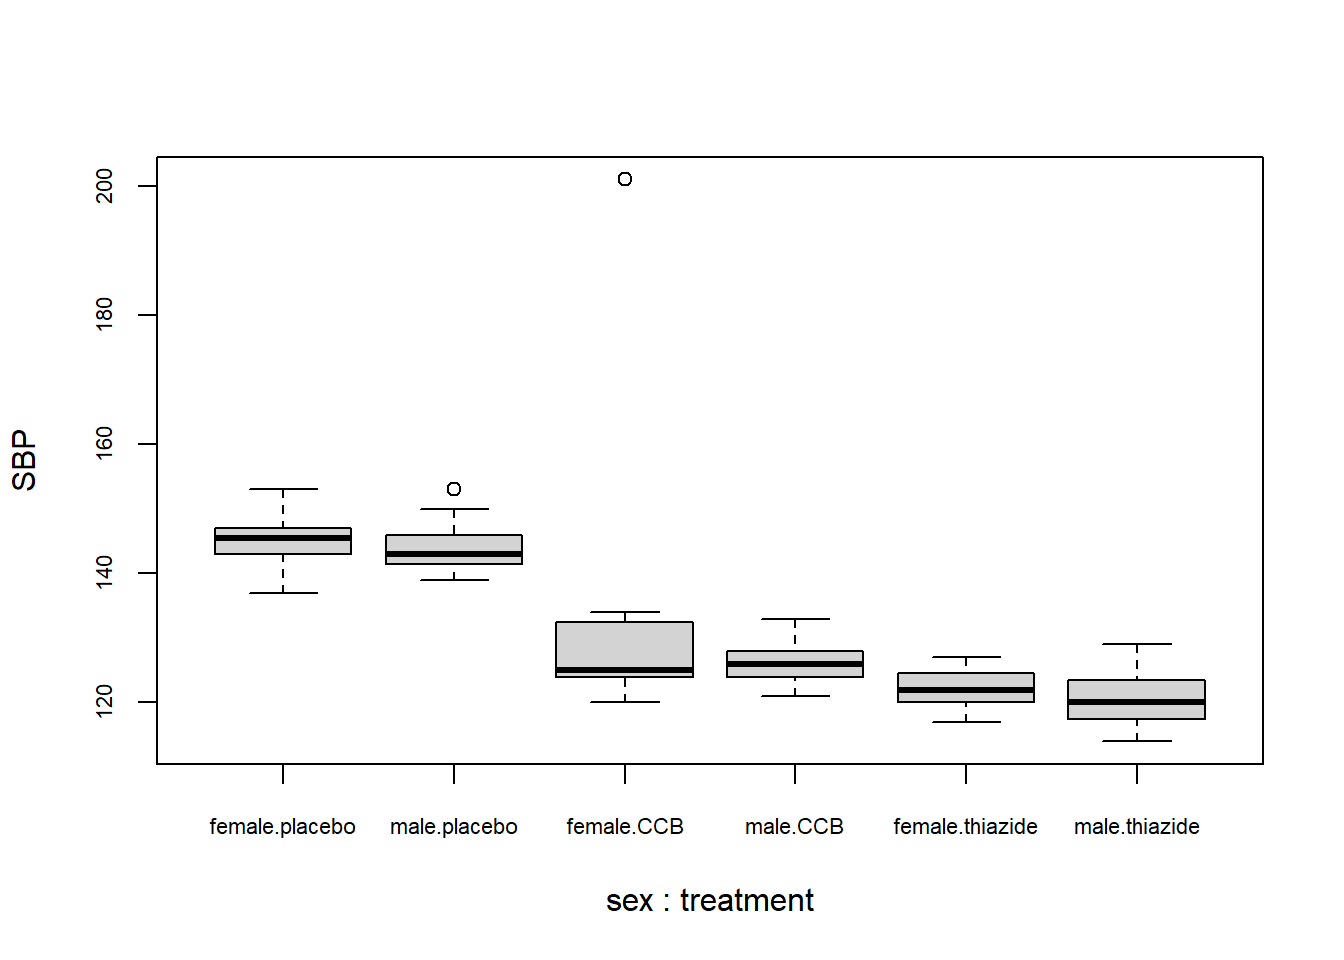
\includegraphics{Tutorials_files/figure-latex/unnamed-chunk-56-1.pdf}

What to look for

Potential Outliers

A boxplot shows either of the following:

\begin{figure}
\centering
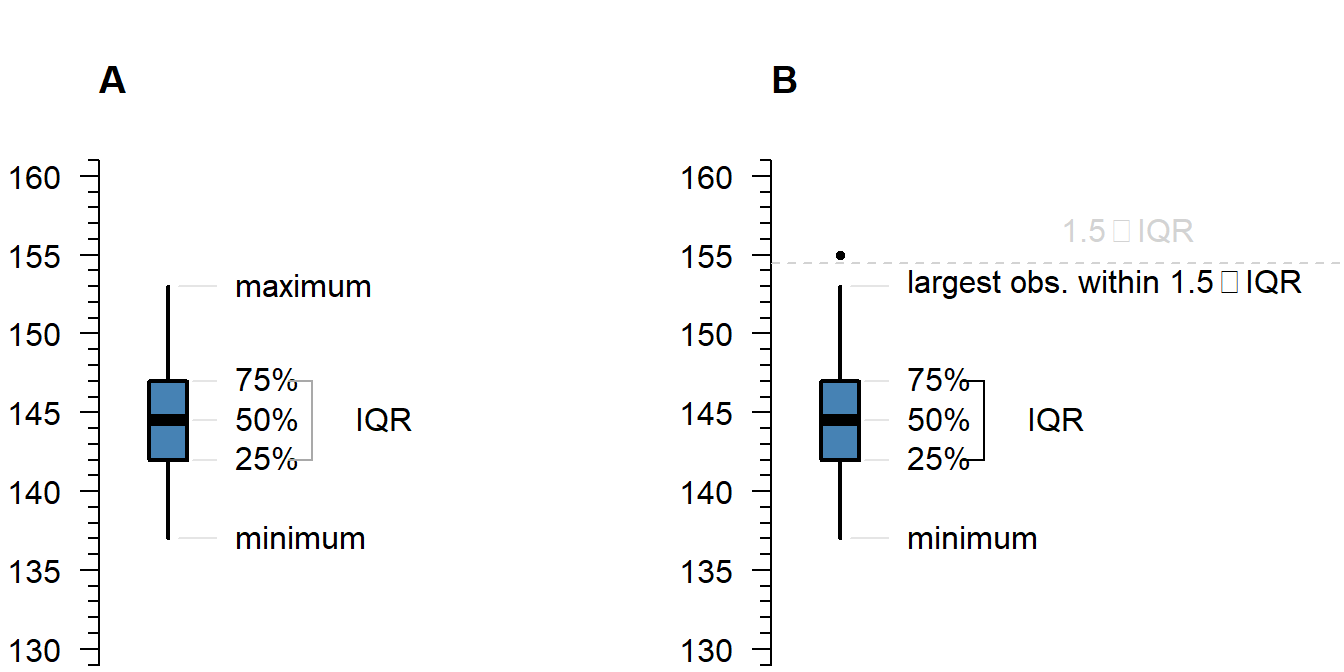
\includegraphics{Tutorials_files/figure-latex/IQR3-1.pdf}
\caption{\label{fig:IQR3}What is displayed in a boxplot in case all observations are within a certain distance from the box (A), or otherwise (B).}
\end{figure}

The interquartile range (IQR) is simply the size of the box. If all observations lie within \(1.5\times\) this range from the box, then the whiskers show the extremes of the data (fig.~\ref{fig:IQR} A). Otherwise, the observations are drawn separately \ref{fig:IQR} B). The IQR is usually not shown in a boxplot, but is used internally to calculate the location of the whiskers and marked observations (if any).

Marked observations are not outliers

This is a common misconception. Though it can be an \emph{indication} of outlyingness, a boxplot alone cannot tell you whether these observations will strongly affect your analysis:

\begin{itemize}
\tightlist
\item
  If you have a large enough sample size, you \emph{will} find more extreme observations, which are eventually drawn outside the IQR. Try running: \texttt{boxplot(rnorm(1000))}
\item
  Skewed values (next section) will almost always show `outliers' in the direction of skew, but these are unlikely to be outliers in the context of an appropriate model for skewed data.
\item
  The \(1.5\times\) IQR rule is nothing special, it is merely convention. A boxplot is just a quick way to visualize numeric values.
\end{itemize}

Skew

Skew means the data-generating process follows a probability distribution that is not symmetric. In a boxplot, skew looks like this:

\begin{figure}
\centering
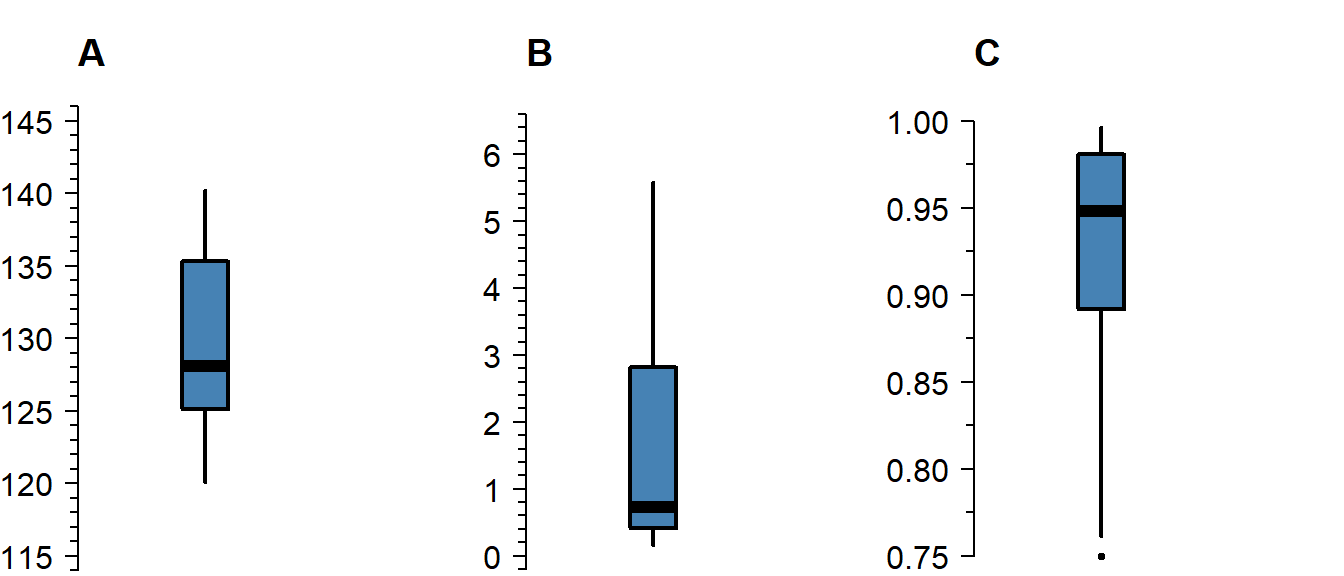
\includegraphics{Tutorials_files/figure-latex/skew3-1.pdf}
\caption{\label{fig:skew3}A boxplot of symmetric (A), right-skewed (B), and left-skewed values.}
\end{figure}

Skew is not necessarily a problem, unless it persists in the residuals of a model that assumes normally distributed errors. For an explanation of skew, see the video on \href{https://youtu.be/jdfG7rKPVNk}{probability distributions }.

Differences Between Groups

A boxplot is not just a nice tool for \emph{yourself} to inspect your data, but is also an effective tool to visually communicate the evidence for difference between groups:

\begin{figure}
\centering
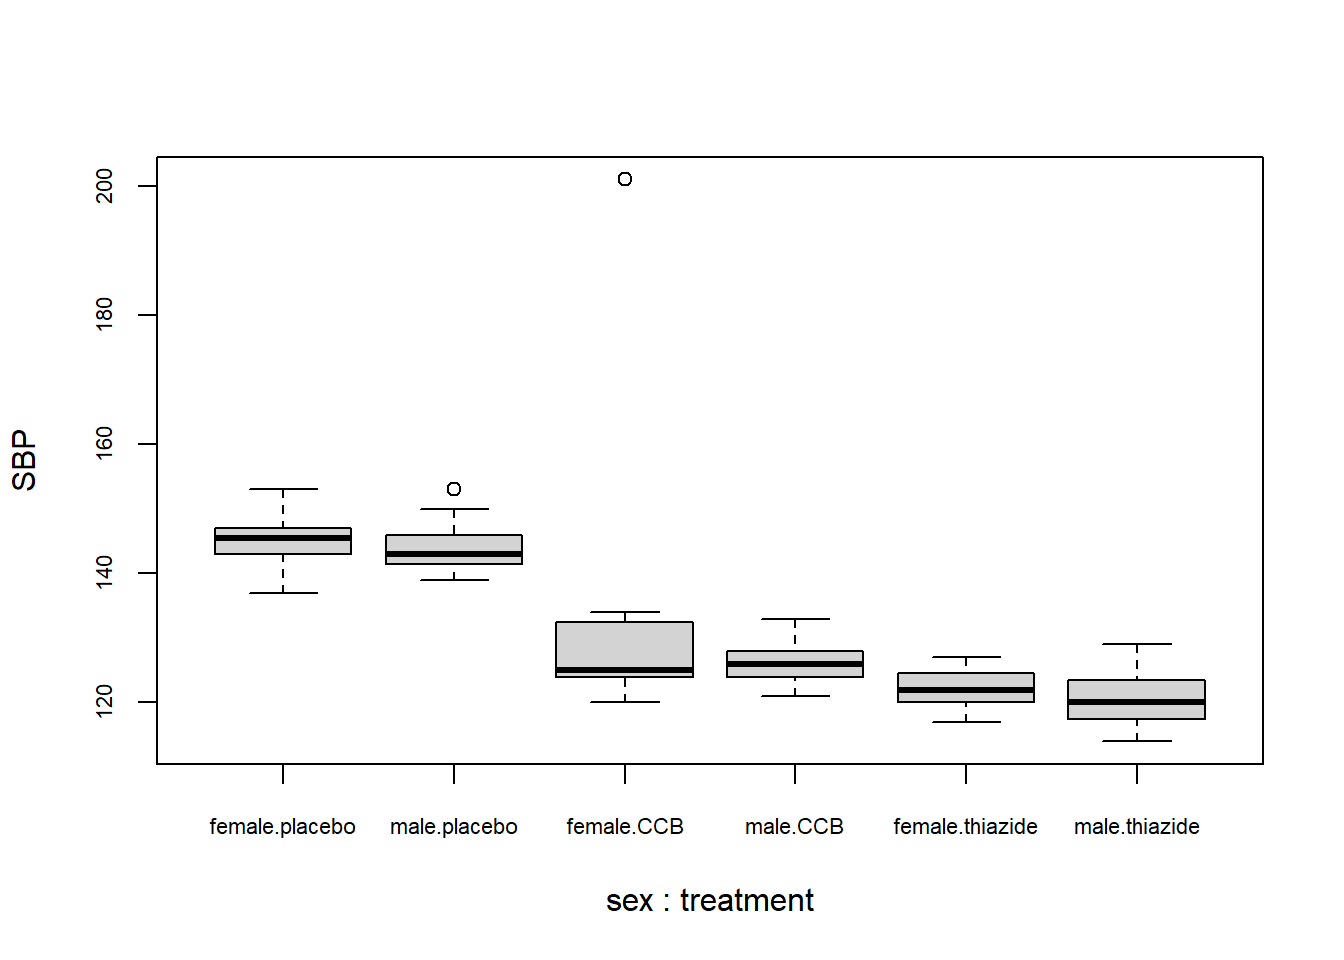
\includegraphics{Tutorials_files/figure-latex/unnamed-chunk-57-1.pdf}
\caption{\label{fig:unnamed-chunk-57}A comparison of systolic blood pressure for different treatments and sex.}
\end{figure}

How to improve your plot

Some basic adjustments that improve any plot:

\begin{itemize}
\tightlist
\item
  Use informative axis labels, with unit of measurement if appropriate;
\item
  Add an informative caption;
\item
  Keep the numbers on the axes horizontal where possible;
\item
  Remove unnecessary plot elements, like the box around the figure.
\end{itemize}

The changes to the code I made below can all be found in the help pages \texttt{?boxplot} and \texttt{?par}. I am also a big fan of the \texttt{eaxis} function from the package \texttt{sfsmisc}. The caption is added as a chunk option (i.e., \texttt{\textasciigrave{}\textasciigrave{}\textasciigrave{}\{r,\ fig.cap\ =\ "..."\}}).

\begin{Shaded}
\begin{Highlighting}[]
\CommentTok{\# Load a package for nice axes}
\FunctionTok{library}\NormalTok{(}\StringTok{"sfsmisc"}\NormalTok{)}
\CommentTok{\# Change the margins (bottom, left, top, right)}
\FunctionTok{par}\NormalTok{(}\AttributeTok{mar =} \FunctionTok{c}\NormalTok{(}\DecValTok{4}\NormalTok{, }\DecValTok{4}\NormalTok{, }\DecValTok{0}\NormalTok{, }\DecValTok{0}\NormalTok{) }\SpecialCharTok{+} \FloatTok{0.1}\NormalTok{)}

\CommentTok{\# Define the locations (helps discern between combinations of groups)}
\NormalTok{where }\OtherTok{\textless{}{-}} \FunctionTok{c}\NormalTok{(}\DecValTok{1}\SpecialCharTok{:}\DecValTok{2}\NormalTok{, }\DecValTok{4}\SpecialCharTok{:}\DecValTok{5}\NormalTok{, }\DecValTok{7}\SpecialCharTok{:}\DecValTok{8}\NormalTok{)}

\CommentTok{\# Create the coordinate system}
\FunctionTok{boxplot}\NormalTok{(SBP }\SpecialCharTok{\textasciitilde{}}\NormalTok{ sex }\SpecialCharTok{+}\NormalTok{ treatment, DF, }\AttributeTok{at =}\NormalTok{ where, }\AttributeTok{axes =} \ConstantTok{FALSE}\NormalTok{,}
        \AttributeTok{pch =} \DecValTok{19}\NormalTok{, }\AttributeTok{cex =} \FloatTok{0.5}\NormalTok{, }\AttributeTok{boxwex =} \FloatTok{0.25}\NormalTok{, }\AttributeTok{staplewex =} \DecValTok{0}\NormalTok{, }
        \AttributeTok{lwd =} \FloatTok{1.5}\NormalTok{, }\AttributeTok{lty =} \DecValTok{1}\NormalTok{, }\AttributeTok{ylim =} \FunctionTok{c}\NormalTok{(}\DecValTok{110}\NormalTok{, }\DecValTok{200}\NormalTok{), }\AttributeTok{xlim =} \FunctionTok{c}\NormalTok{(}\FloatTok{0.5}\NormalTok{, }\DecValTok{12}\NormalTok{),}
        \AttributeTok{xlab =} \StringTok{"Treatment"}\NormalTok{, }\AttributeTok{ylab =} \StringTok{"Systolic blood pressure (mmHg)"}\NormalTok{)}

\CommentTok{\# Add axes}
\FunctionTok{axis}\NormalTok{(}\DecValTok{1}\NormalTok{, }\FunctionTok{c}\NormalTok{(}\FloatTok{1.5}\NormalTok{, }\FloatTok{4.5}\NormalTok{, }\FloatTok{7.5}\NormalTok{), }\FunctionTok{levels}\NormalTok{(DF}\SpecialCharTok{$}\NormalTok{treatment))}
\FunctionTok{eaxis}\NormalTok{(}\DecValTok{2}\NormalTok{)}

\CommentTok{\# Add a lightgrey background}
\FunctionTok{polygon}\NormalTok{(}\AttributeTok{x =} \FunctionTok{c}\NormalTok{(}\SpecialCharTok{{-}}\DecValTok{1}\NormalTok{, }\DecValTok{9}\NormalTok{, }\DecValTok{9}\NormalTok{, }\SpecialCharTok{{-}}\DecValTok{1}\NormalTok{, }\SpecialCharTok{{-}}\DecValTok{1}\NormalTok{), }\AttributeTok{y =} \FunctionTok{c}\NormalTok{(}\DecValTok{100}\NormalTok{, }\DecValTok{100}\NormalTok{, }\DecValTok{210}\NormalTok{, }\DecValTok{210}\NormalTok{, }\DecValTok{100}\NormalTok{), }\AttributeTok{col =} \StringTok{"grey95"}\NormalTok{,}
        \AttributeTok{border =} \ConstantTok{NA}\NormalTok{)}

\CommentTok{\# Add a simple grid}
\FunctionTok{abline}\NormalTok{(}\AttributeTok{h =} \FunctionTok{seq}\NormalTok{(}\DecValTok{100}\NormalTok{, }\DecValTok{200}\NormalTok{, }\DecValTok{10}\NormalTok{), }\AttributeTok{col =} \StringTok{"white"}\NormalTok{, }\AttributeTok{lwd =} \DecValTok{1}\NormalTok{)}
\FunctionTok{abline}\NormalTok{(}\AttributeTok{h =} \FunctionTok{seq}\NormalTok{(}\DecValTok{100}\NormalTok{, }\DecValTok{200}\NormalTok{, }\DecValTok{20}\NormalTok{), }\AttributeTok{col =} \StringTok{"white"}\NormalTok{, }\AttributeTok{lwd =} \FloatTok{1.5}\NormalTok{)}

\CommentTok{\# Define two colors (picked from colorbrewer2.org):}
\NormalTok{cols }\OtherTok{\textless{}{-}} \FunctionTok{c}\NormalTok{(}\StringTok{"\#fb9a99"}\NormalTok{, }\StringTok{"\#a6cee3"}\NormalTok{)}

\CommentTok{\# Redraw the boxplots on top}
\FunctionTok{boxplot}\NormalTok{(SBP }\SpecialCharTok{\textasciitilde{}}\NormalTok{ sex }\SpecialCharTok{+}\NormalTok{ treatment, DF, }\AttributeTok{at =}\NormalTok{ where, }\AttributeTok{axes =} \ConstantTok{FALSE}\NormalTok{,}
        \AttributeTok{boxwex =} \FloatTok{0.25}\NormalTok{, }\AttributeTok{staplewex =} \DecValTok{0}\NormalTok{, }\AttributeTok{col =}\NormalTok{ cols, }\AttributeTok{add =} \ConstantTok{TRUE}\NormalTok{, }
        \AttributeTok{pch =} \DecValTok{19}\NormalTok{, }\AttributeTok{cex =} \FloatTok{0.5}\NormalTok{, }\AttributeTok{lwd =} \FloatTok{1.5}\NormalTok{, }\AttributeTok{lty =} \DecValTok{1}\NormalTok{)}

\CommentTok{\# Add a legend}
\FunctionTok{legend}\NormalTok{(}\StringTok{"topright"}\NormalTok{, }\AttributeTok{legend =} \FunctionTok{levels}\NormalTok{(DF}\SpecialCharTok{$}\NormalTok{sex), }\AttributeTok{pch =} \DecValTok{15}\NormalTok{, }\AttributeTok{col =}\NormalTok{ cols, }\AttributeTok{bty =} \StringTok{"n"}\NormalTok{)}

\CommentTok{\# Restore the default margins for subsequent plots}
\FunctionTok{par}\NormalTok{(}\AttributeTok{mar =} \FunctionTok{c}\NormalTok{(}\DecValTok{5}\NormalTok{, }\DecValTok{4}\NormalTok{, }\DecValTok{4}\NormalTok{, }\DecValTok{3}\NormalTok{) }\SpecialCharTok{+} \FloatTok{0.1}\NormalTok{)}
\end{Highlighting}
\end{Shaded}

\begin{figure}
\centering
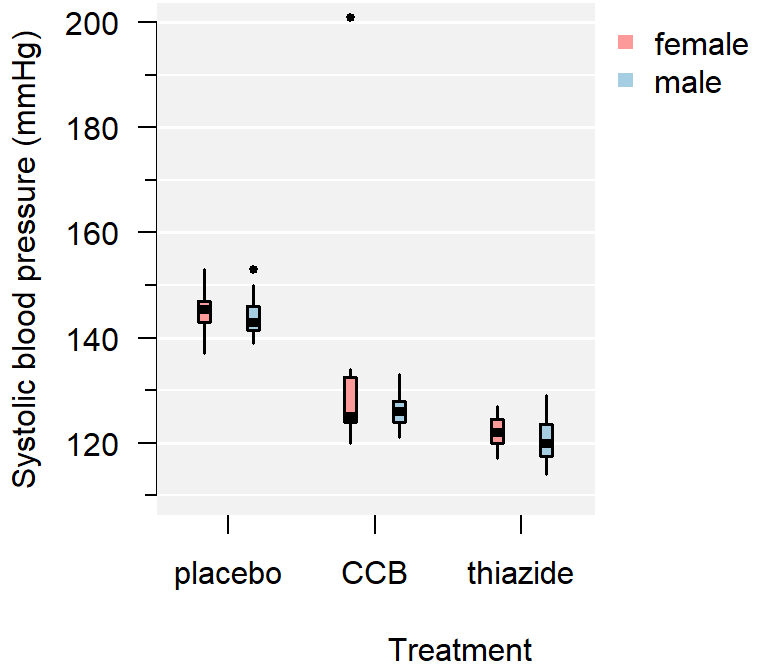
\includegraphics{Tutorials_files/figure-latex/unnamed-chunk-59-1.pdf}
\caption{\label{fig:unnamed-chunk-59}A comparison of systolic blood pressure for three groups.}
\end{figure}

From the plot you can conclude:

\begin{itemize}
\tightlist
\item
  There appears to be a clear outlier in the female CCB group;
\item
  None of the groups appear skewed;
\item
  Both the CCB and thiazide group have substantially lower blood pressure than the control, with thiazide appearing the lowest;
\item
  This difference appears to be similar for males and females;
\item
  Systolic blood pressure does not appear to differ by sex at all;
\item
  The variance of all groups is similar, because the boxes are similarly sized.
\end{itemize}

This is just a sample, so whether this difference is \emph{significant}, should be determined with a test.

Alternative: Violin plot

A more modern take on the boxplot is a \textbf{violin plot}. It combines a boxplot and a density plot. This type of visualization is richer in information than just a boxplot, but it is only meaningful if you have enough observations per group (e.g., \textgreater10):

\begin{Shaded}
\begin{Highlighting}[]
\FunctionTok{library}\NormalTok{(}\StringTok{"vioplot"}\NormalTok{) }\CommentTok{\# install if missing}
\FunctionTok{vioplot}\NormalTok{(SBP }\SpecialCharTok{\textasciitilde{}}\NormalTok{ treatment, DF)}
\end{Highlighting}
\end{Shaded}

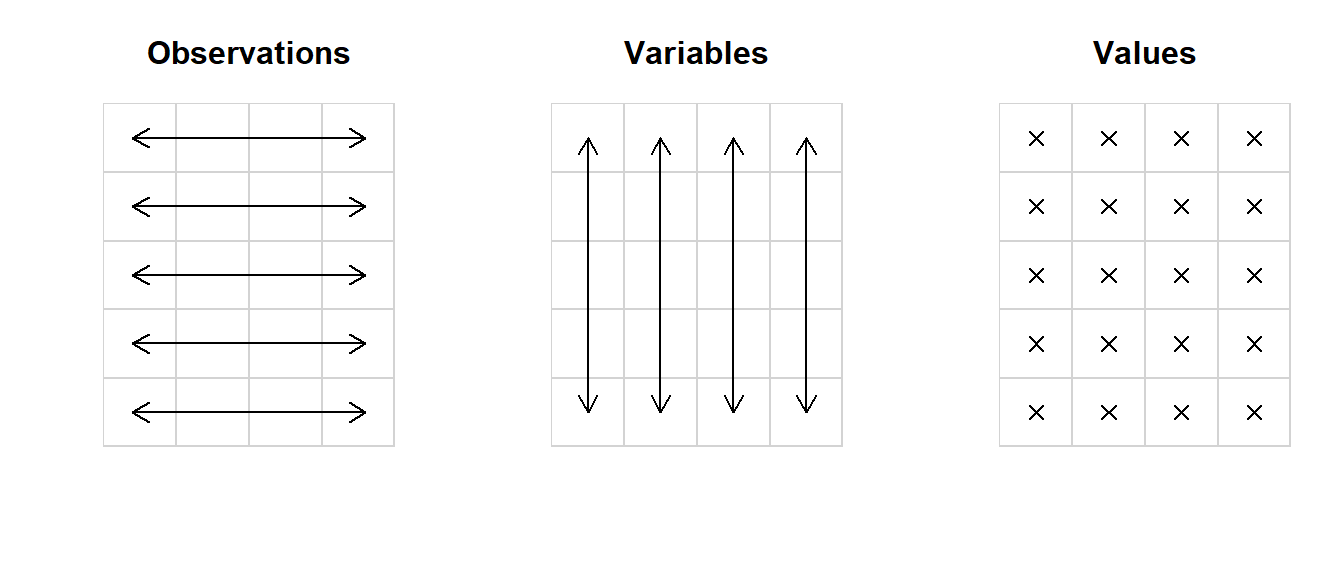
\includegraphics{Tutorials_files/figure-latex/unnamed-chunk-60-1.pdf}

How to interpret a violin plot

Here is a breakdown of the components shown in a violin plot:

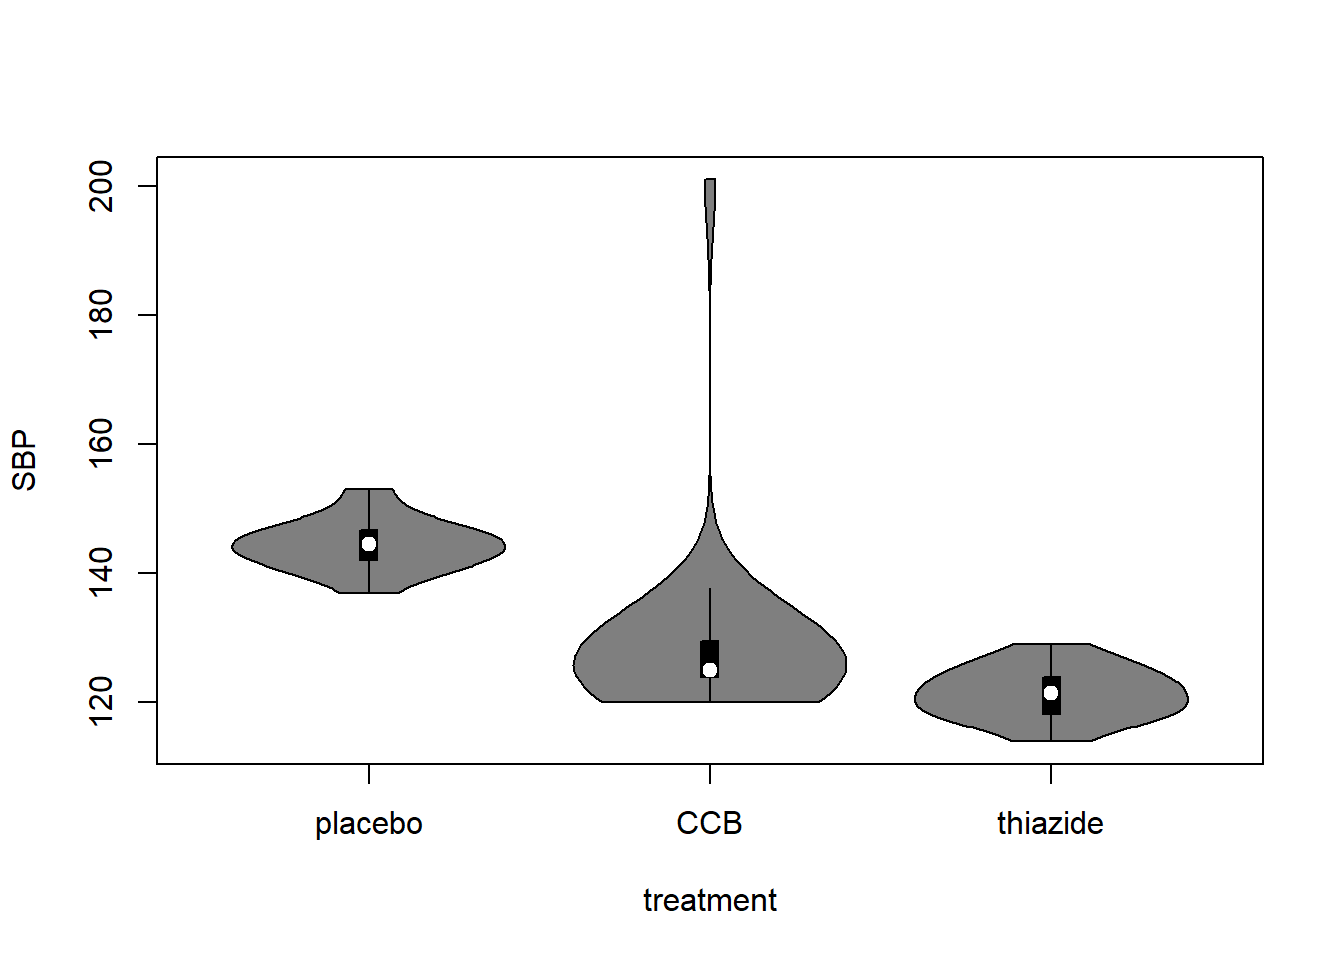
\includegraphics{Tutorials_files/figure-latex/unnamed-chunk-61-1.pdf}

The density plot, if you are unfamiliar with it, is like a continuous version of a histogram. It shows which values are more and less likely in the sample.

\hypertarget{analyze-the-data}{%
\section{Analyze the Data}\label{analyze-the-data}}

Summary (code)

\begin{Shaded}
\begin{Highlighting}[]
\CommentTok{\# Load packages used (install if missing)}
\FunctionTok{require}\NormalTok{(}\StringTok{"car"}\NormalTok{)}
\FunctionTok{require}\NormalTok{(}\StringTok{"emmeans"}\NormalTok{)}

\CommentTok{\# Fit the model}
\NormalTok{LM }\OtherTok{\textless{}{-}} \FunctionTok{lm}\NormalTok{(SBP }\SpecialCharTok{\textasciitilde{}}\NormalTok{ treatment, DF)}

\CommentTok{\# Perform visual diagnostics}
\FunctionTok{par}\NormalTok{(}\AttributeTok{mfrow =} \FunctionTok{c}\NormalTok{(}\DecValTok{2}\NormalTok{, }\DecValTok{2}\NormalTok{))   }\CommentTok{\# Plot in a 2x2 grid}
\FunctionTok{plot}\NormalTok{(LM, }\AttributeTok{which =} \DecValTok{1}\NormalTok{)    }\CommentTok{\# Residuals vs fitted}
\FunctionTok{qqPlot}\NormalTok{(LM, }\AttributeTok{reps =} \FloatTok{1e4}\NormalTok{) }\CommentTok{\# QQ{-}plot}
\FunctionTok{plot}\NormalTok{(LM, }\AttributeTok{which =} \DecValTok{3}\NormalTok{)    }\CommentTok{\# Scale{-}location}
\FunctionTok{plot}\NormalTok{(LM, }\AttributeTok{which =} \DecValTok{4}\NormalTok{)    }\CommentTok{\# Cook\textquotesingle{}s distance}
\FunctionTok{par}\NormalTok{(}\AttributeTok{mfrow =} \FunctionTok{c}\NormalTok{(}\DecValTok{1}\NormalTok{, }\DecValTok{1}\NormalTok{))   }\CommentTok{\# Restore the default}

\CommentTok{\# Obs. 31 appears to be outlying:}
\NormalTok{DF[}\DecValTok{31}\NormalTok{, ]}

\CommentTok{\# Omitting this observation can be justified based on age}
\NormalTok{LM }\OtherTok{\textless{}{-}} \FunctionTok{lm}\NormalTok{(SBP }\SpecialCharTok{\textasciitilde{}}\NormalTok{ treatment, DF[}\SpecialCharTok{{-}}\DecValTok{31}\NormalTok{, ])}

\CommentTok{\# Perform an omnibus test}
\FunctionTok{summary.aov}\NormalTok{(LM)}

\CommentTok{\# If the omnibus test is significant, perform a post{-}hoc}
\NormalTok{EMM }\OtherTok{\textless{}{-}} \FunctionTok{emmeans}\NormalTok{(LM, }\AttributeTok{specs =} \StringTok{"treatment"}\NormalTok{)}
\FunctionTok{pairs}\NormalTok{(EMM)}

\CommentTok{\# Visualize the post hoc (see the emmeans vignette)}
\FunctionTok{plot}\NormalTok{(EMM, }\AttributeTok{comparisons =} \ConstantTok{TRUE}\NormalTok{)}
\end{Highlighting}
\end{Shaded}

Fit the Model

In the example, we are only interested in the effect of \texttt{treatment}. For a single grouping variable, use:

\begin{Shaded}
\begin{Highlighting}[]
\NormalTok{LM }\OtherTok{\textless{}{-}} \FunctionTok{lm}\NormalTok{(SBP }\SpecialCharTok{\textasciitilde{}}\NormalTok{ treatment, DF)}
\end{Highlighting}
\end{Shaded}

The general notation is \texttt{Outcome\ \textasciitilde{}\ GroupingVariable,\ Data}. Adding more grouping variables is simple, but model selection is not, so two-way and multi-way ANOVA are explained separately in the \protect\hyperlink{twowaymultiway}{next chapter}.

Why use a linear model (\texttt{lm})?

\emph{(The short answer is that ANOVA is linear and we decided to use \texttt{emmeans} throughout the tutorials for consistency.)}

Linear means that we can express the model as intercept and slope(s):

\[\text{intercept} + \text{slope} \times \text{explanatory variable}\]

Categorical explanatory variables, like \texttt{treatment}, can be represented by \href{https://youtu.be/3ZY9OSXmOrU?t=657}{dummy variables }:

\[
\begin{aligned}
  x_1 &= 
    \begin{cases}
      1 \; \text{if CCB} \\
      0 \; \text{otherwise}
    \end{cases} \\ \\
  x_2 &= 
    \begin{cases}
      1 \; \text{if thiazide} \\
      0 \; \text{otherwise}
    \end{cases}
\end{aligned}
\]
These variables are equal to \(1\) if the observation belongs to that group and \(0\) otherwise. Our example model then becomes:

\[\text{SBP} = \text{intercept} + \text{slope} \cdot x_1 + \text{slope} \cdot x_2\]

That might look confusing at first, because this isn't a slope in the everyday meaning of the word. But all that `slope' means in statistics is the extent to which the outcome changes, if the explanatory variable increases by \(1\). For example, \textbf{if you belong to the thiazide group}, then the equation becomes:

\[\text{SBP} = \text{intercept} + \text{slope} \cdot 0 + \text{slope} \cdot 1\]

\textbf{If you belong to the control group}, the equation becomes:

\[\text{SBP} = \text{intercept} + \text{slope} \cdot 0 + \text{slope} \cdot 0\]

Which is simply the value of the intercept.

Hence, comparing group means is the same as fitting a linear model with only dummy variables. This is useful for a number of reasons, but primarily:

\begin{itemize}
\tightlist
\item
  We can use the same notation for everything from \(t\)-test to ANCOVA;
\item
  We can use \texttt{lm}, which is supported by far more functions than \texttt{aov};
\item
  We can easily correct for \href{https://youtu.be/RUX94txw4Qo}{multiple testing }. \emph{(The traditional \texttt{aov} + \texttt{TukeyHSD} approach does not correct for two-way or multi-way ANOVA.)}
\end{itemize}

Perform Diagnostics

The calculation of confidence intervals and \(p\)-values is based on several assumptions. If these are not reasonable, conclusions drawn from the analysis are invalid.

Additionally, outliers can have a strong influence on the estimates and \(p\)-values, so you should always check and decide whether outlying observations are genuine, or outlying for reasons that warrant exclusion.

Checking assumptions and outlyingness can be done trough \href{https://youtu.be/upJJmfSbBuQ}{visual diagnostics }.

\begin{Shaded}
\begin{Highlighting}[]
\FunctionTok{require}\NormalTok{(}\StringTok{"car"}\NormalTok{)         }\CommentTok{\# Install if missing}
\FunctionTok{par}\NormalTok{(}\AttributeTok{mfrow =} \FunctionTok{c}\NormalTok{(}\DecValTok{2}\NormalTok{, }\DecValTok{2}\NormalTok{))   }\CommentTok{\# Plot in a 2x2 grid}
\FunctionTok{plot}\NormalTok{(LM, }\AttributeTok{which =} \DecValTok{1}\NormalTok{)    }\CommentTok{\# Residuals vs fitted}
\FunctionTok{qqPlot}\NormalTok{(LM, }\AttributeTok{reps =} \FloatTok{1e4}\NormalTok{) }\CommentTok{\# QQ{-}plot}
\FunctionTok{plot}\NormalTok{(LM, }\AttributeTok{which =} \DecValTok{3}\NormalTok{)    }\CommentTok{\# Scale{-}location}
\FunctionTok{plot}\NormalTok{(LM, }\AttributeTok{which =} \DecValTok{4}\NormalTok{)    }\CommentTok{\# Cook\textquotesingle{}s distance}
\FunctionTok{par}\NormalTok{(}\AttributeTok{mfrow =} \FunctionTok{c}\NormalTok{(}\DecValTok{1}\NormalTok{, }\DecValTok{1}\NormalTok{))   }\CommentTok{\# Restore the default}
\end{Highlighting}
\end{Shaded}

Show output

\emph{(For general advice on diagnostic plots, see the \href{https://youtu.be/upJJmfSbBuQ}{video }.)}

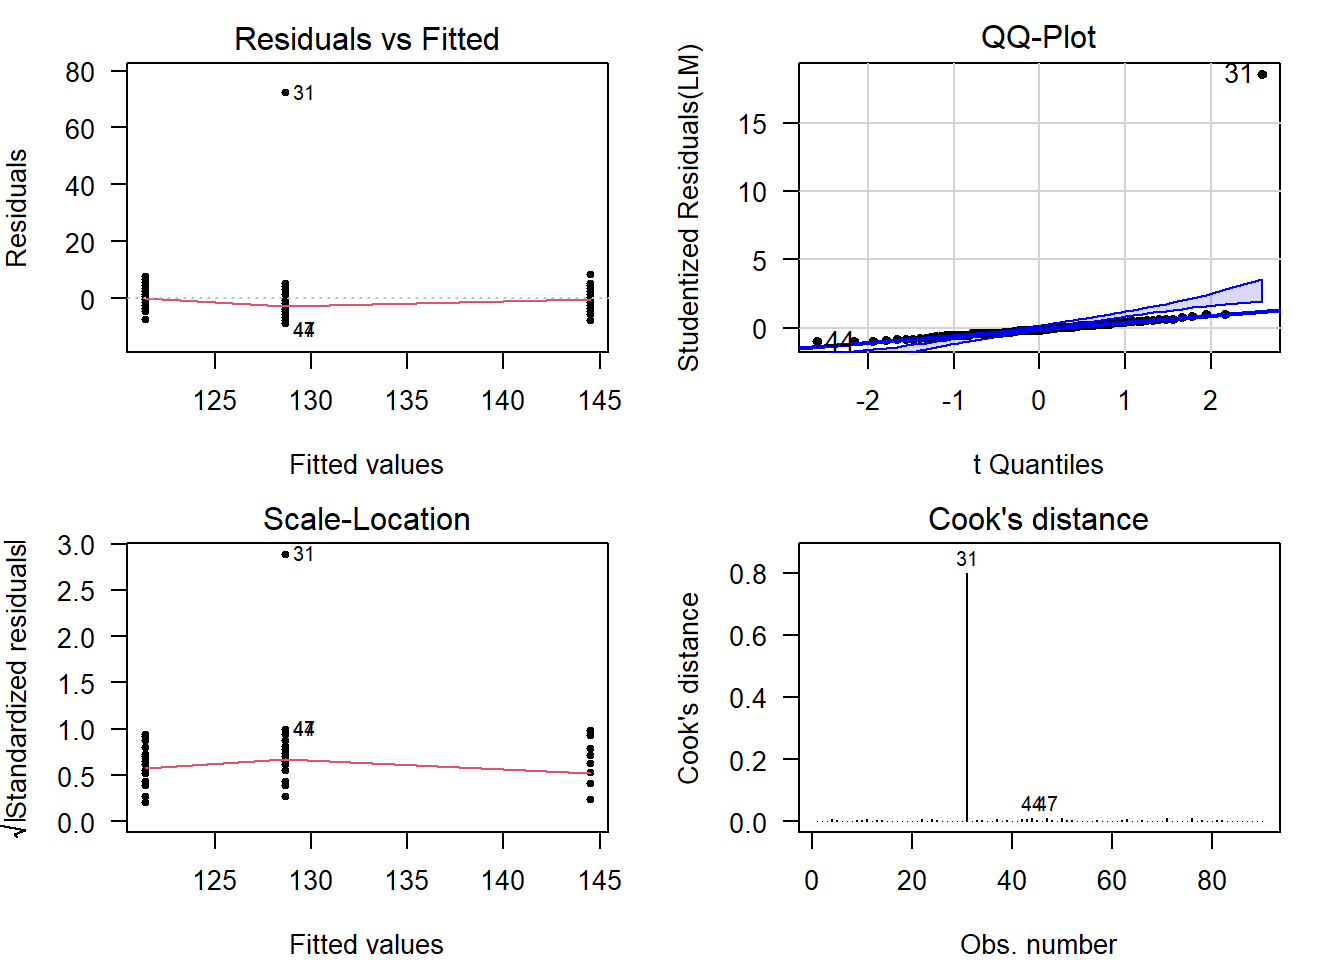
\includegraphics{Tutorials_files/figure-latex/unnamed-chunk-65-1.pdf}

The visual diagnostics confirm what was already visible in the boxplots, there is an outlier (\#31) visible in each of the plots. Its Cook's distance is well over \(0.5\).

Let's see what the diagnostics would look like without this observation:

\begin{Shaded}
\begin{Highlighting}[]
\CommentTok{\# Fit a model on the data, excluding obs. 31}
\NormalTok{LM2 }\OtherTok{\textless{}{-}} \FunctionTok{lm}\NormalTok{(SBP }\SpecialCharTok{\textasciitilde{}}\NormalTok{ treatment, DF[}\SpecialCharTok{{-}}\DecValTok{31}\NormalTok{, ])}

\CommentTok{\# Run the diagnostics}
\FunctionTok{par}\NormalTok{(}\AttributeTok{mfrow =} \FunctionTok{c}\NormalTok{(}\DecValTok{2}\NormalTok{, }\DecValTok{2}\NormalTok{))    }\CommentTok{\# Plot in a 2x2 grid}
\FunctionTok{plot}\NormalTok{(LM2, }\AttributeTok{which =} \DecValTok{1}\NormalTok{)    }\CommentTok{\# Residuals vs fitted}
\FunctionTok{qqPlot}\NormalTok{(LM2, }\AttributeTok{reps =} \FloatTok{1e4}\NormalTok{) }\CommentTok{\# QQ{-}plot}
\FunctionTok{plot}\NormalTok{(LM2, }\AttributeTok{which =} \DecValTok{3}\NormalTok{)    }\CommentTok{\# Scale{-}location}
\FunctionTok{plot}\NormalTok{(LM2, }\AttributeTok{which =} \DecValTok{4}\NormalTok{)    }\CommentTok{\# Cook\textquotesingle{}s distance}
\FunctionTok{par}\NormalTok{(}\AttributeTok{mfrow =} \FunctionTok{c}\NormalTok{(}\DecValTok{1}\NormalTok{, }\DecValTok{1}\NormalTok{))    }\CommentTok{\# Restore the default}
\end{Highlighting}
\end{Shaded}

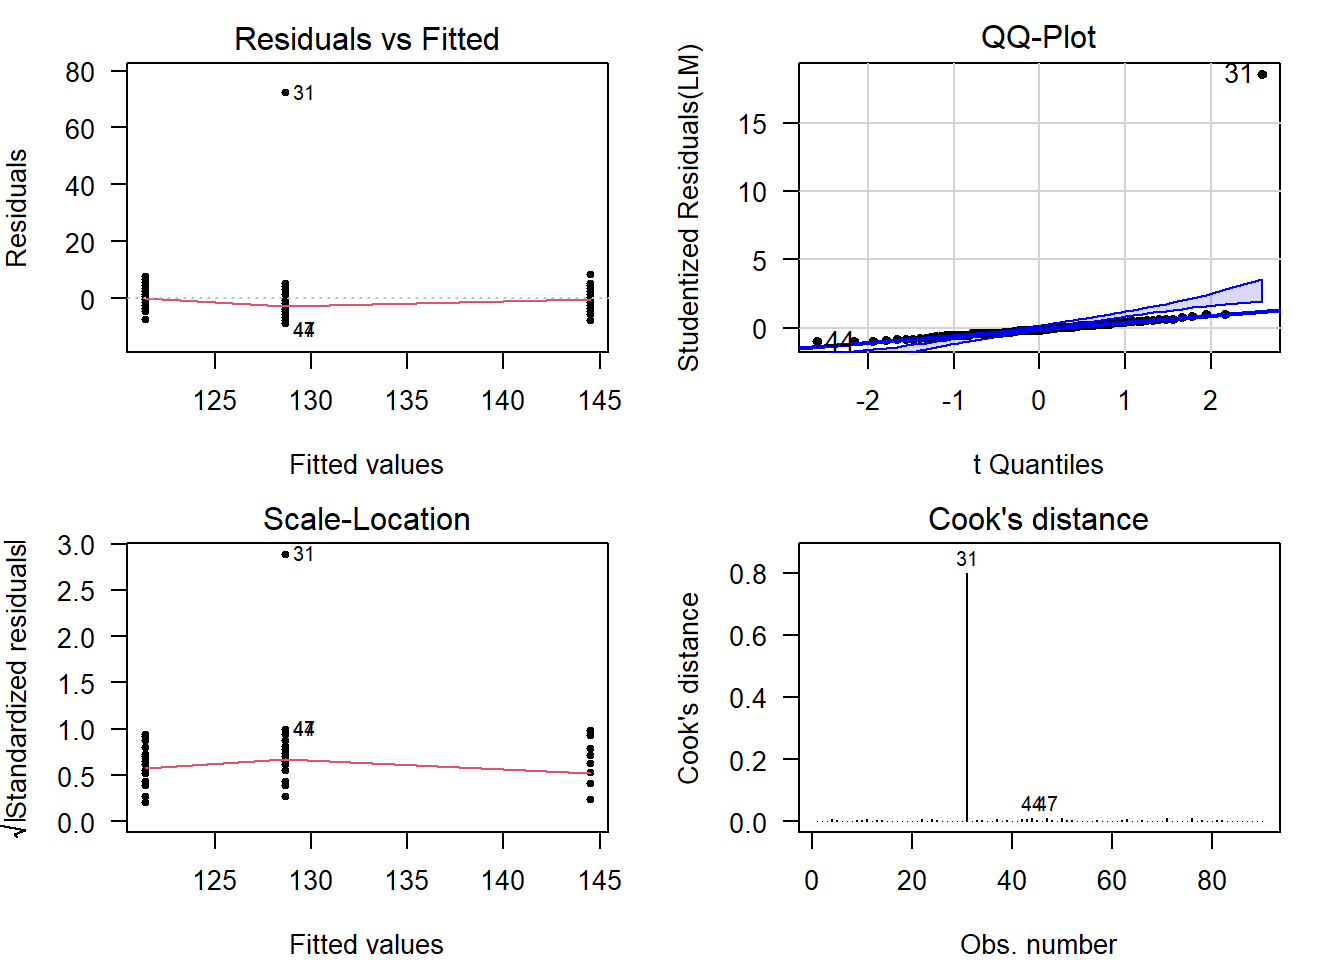
\includegraphics{Tutorials_files/figure-latex/unnamed-chunk-67-1.pdf}

Now the diagnostics look fine. If you are concerned about the staircase in the QQ-plot, that is an artifact of the way these data were collected: Systolic blood pressure was rounded to whole numbers, but the actual underlying values can reasonably be assumed to be normally distributed within groups.

Significance tests for assumptions

All significance tests can produce false positives. Always judge the severity of any supposed problems with \emph{visual} diagnostics.

In cases where you are not sure an assumption is violated, it is possible to conduct a test.

Normality

Deviations from conditional normality can be formally tested using a variety of tests, all of which have different sensitivities to different aspects of the normal probability distribution. Commonly used is the Shapiro--Wilks test, which is particularly sensitive to skew and light-tailedness.\citep{ShapiroSensitivities}

\begin{Shaded}
\begin{Highlighting}[]
\FunctionTok{shapiro.test}\NormalTok{(}\FunctionTok{residuals}\NormalTok{(LM))}
\end{Highlighting}
\end{Shaded}

Show output

\begin{verbatim}
## 
##  Shapiro-Wilk normality test
## 
## data:  residuals(LM)
## W = 0.48457, p-value = 3.255e-16
\end{verbatim}

The residuals differ significantly from a theoretical normal distribution (\(p = 3.23 \cdot 10^{-16}\)), though this is likely due to the outlier seen in the visual diagnostics, which is something you can try out:

\begin{Shaded}
\begin{Highlighting}[]
\NormalTok{LM2 }\OtherTok{\textless{}{-}} \FunctionTok{lm}\NormalTok{(SBP }\SpecialCharTok{\textasciitilde{}}\NormalTok{ treatment, DF[}\SpecialCharTok{{-}}\DecValTok{31}\NormalTok{, ])}
\FunctionTok{shapiro.test}\NormalTok{(}\FunctionTok{residuals}\NormalTok{(LM2))}
\end{Highlighting}
\end{Shaded}

\begin{verbatim}
## 
##  Shapiro-Wilk normality test
## 
## data:  residuals(LM2)
## W = 0.97918, p-value = 0.1634
\end{verbatim}

And indeed, now there is no detected deviation from normality anymore.

This does not demonstrate the values are normally distributed

This is a common misconception. All we found is a lack of evidence against normality. But for these values to be normally distributed, they would need to range all the way from \(-\infty\) to \(\infty\), which is obviously not realistic for blood pressure.

\emph{Also see: \href{https://stats.stackexchange.com/a/85914/176202}{Why do statisticians say a non-significant result means ``you can't reject the null'' as opposed to accepting the null hypothesis?}}

Constant Variance

A robust test for non-constant variance that is not sensitive to other common issues like outliers and non-normality is the Breusch--Pagan test:

\begin{Shaded}
\begin{Highlighting}[]
\FunctionTok{require}\NormalTok{(}\StringTok{"lmtest"}\NormalTok{) }\CommentTok{\# Install if missing}
\FunctionTok{bptest}\NormalTok{(LM)}
\end{Highlighting}
\end{Shaded}

Show output

\begin{verbatim}
## 
##  studentized Breusch-Pagan test
## 
## data:  LM
## BP = 2.2161, df = 2, p-value = 0.3302
\end{verbatim}

As expected from the visual diagnostics, group variances are not significantly different (\(p = 0.330\)).

This does not demonstrate the groups have equal variance

This is a common misconception. All we found is a lack of evidence \emph{against} equal variance.

\emph{Also see: \href{https://stats.stackexchange.com/a/85914/176202}{Why do statisticians say a non-significant result means ``you can't reject the null'' as opposed to accepting the null hypothesis?}}

Outliers

A test for outlyingness is included in the \texttt{car} package:

\begin{Shaded}
\begin{Highlighting}[]
\FunctionTok{require}\NormalTok{(}\StringTok{"car"}\NormalTok{)}
\FunctionTok{outlierTest}\NormalTok{(LM)}
\end{Highlighting}
\end{Shaded}

Show output

\begin{verbatim}
##    rstudent unadjusted p-value Bonferroni p
## 31 18.55085         8.3005e-32   7.4705e-30
\end{verbatim}

The test looks at every individual residual and whether it might be outlying. That of course, poses a major multiple testing issue, so the rersulting \(p\)-values are adjusted for this. When looking for outliyngness, always check the \emph{adjusted} \(p\)-value.

In this case, the test is significant (\(p_{\text{adj}} = 7.47 \cdot 10^{-30}\)) and observation 31 is again pointed out to be the offending observation.

The \texttt{car} package contains another set of residual plots specifically to assess outlyingness:

\begin{Shaded}
\begin{Highlighting}[]
\FunctionTok{influenceIndexPlot}\NormalTok{(LM)}
\end{Highlighting}
\end{Shaded}

Show output

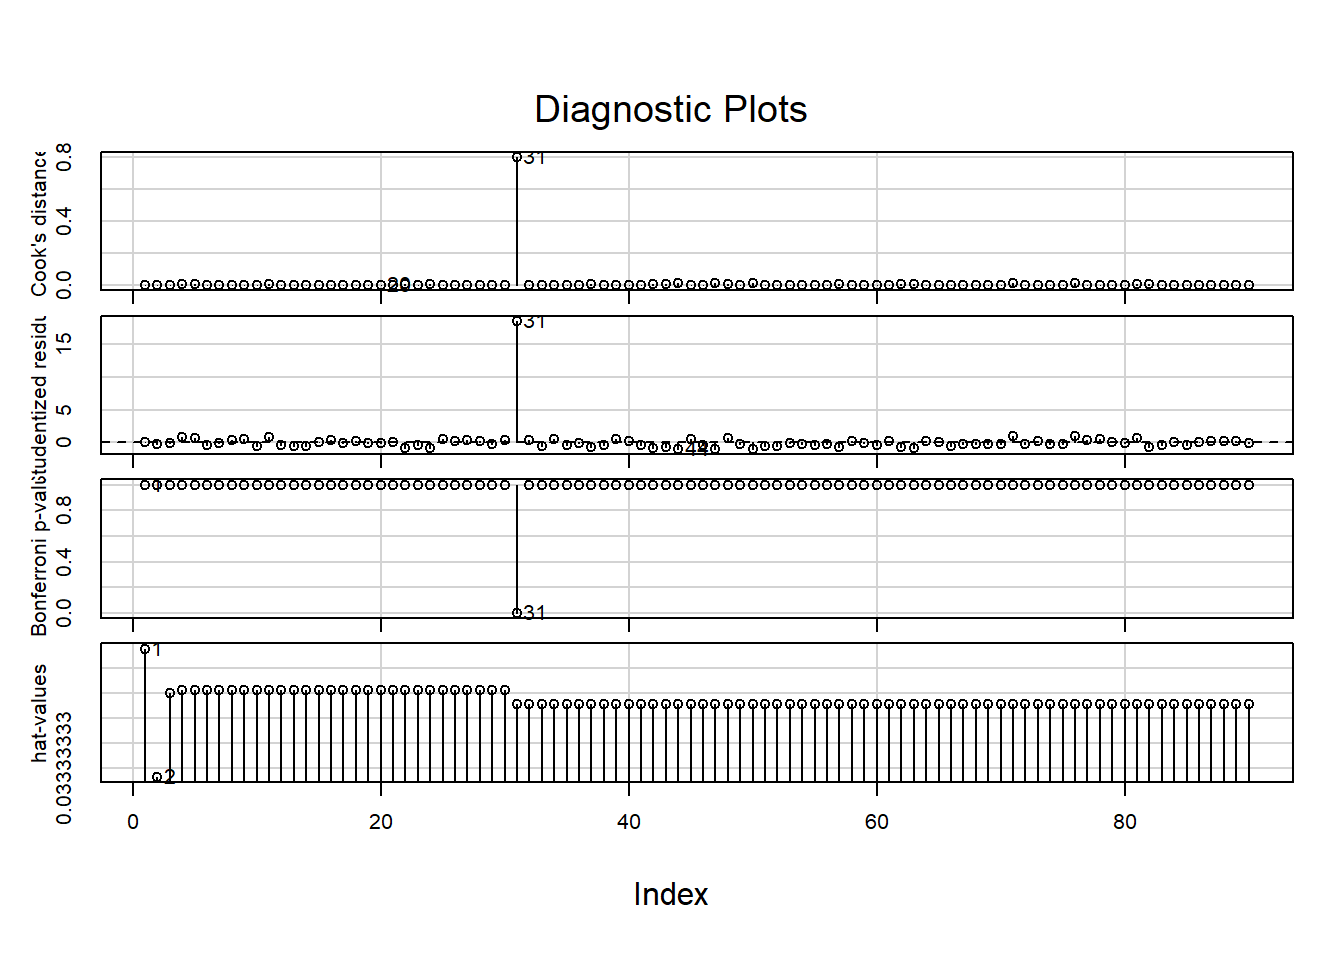
\includegraphics{Tutorials_files/figure-latex/unnamed-chunk-76-1.pdf}

These show, in order:

\begin{itemize}
\tightlist
\item
  The Cook's distance; \emph{(Greater than \(0.5\) is noteworthy, greater than \(1.0\) is outlying.)}
\item
  The studentized residuals; \emph{(Divided by their standard deviation for standardized interpretation.)}
\item
  \(P\)-values for outlyingess; \emph{(Corrected for \href{https://youtu.be/RUX94txw4Qo}{multiple testing}.)}
\item
  The hat-values. \emph{(A measure of relative influence.)}
\end{itemize}

Observation 31 is again pointed out.

What to do if an assumption is violated?

Unfortunately this is where statistics ends. Uninstall R and RStudio from your computer and find a different profession. (\ldots) under construction.

xxxxxxxxxxxxxxxxx

Perform an Omnibus Test

To print a classic ANOVA table, run the following:

\begin{Shaded}
\begin{Highlighting}[]
\FunctionTok{summary.aov}\NormalTok{(LM)}
\end{Highlighting}
\end{Shaded}

Show output

\begin{verbatim}
##             Df Sum Sq Mean Sq F value   Pr(>F)    
## treatment    2   8391    4196   53.96 5.77e-16 ***
## Residuals   87   6765      78                     
## ---
## Signif. codes:  0 '***' 0.001 '**' 0.01 '*' 0.05 '.' 0.1 ' ' 1
\end{verbatim}

The omnibus test is significant (\(F = 54.0\), \(p = 5.77 \cdot 10^{-16}\)), meaning there is a significant difference among group means. For a full explanation of the table above, see the \href{https://youtu.be/BFB4o4uBgPs}{video }.

\hypertarget{results-ANOVA}{%
\section{Correctly Phrase the Results}\label{results-ANOVA}}

We used ANOVA because we don't know what we're doing.

\hypertarget{incorporating-this-in-a-paper-2}{%
\section{Incorporating This in a Paper}\label{incorporating-this-in-a-paper-2}}

\hypertarget{twowaymultiway}{%
\chapter{Two-Way \& Multi-Way ANOVA}\label{twowaymultiway}}

\ldots{}

\begin{center}\rule{0.5\linewidth}{0.5pt}\end{center}

\ldots{}

\hypertarget{linear-model}{%
\chapter{Linear Model}\label{linear-model}}

\ldots{}

\begin{center}\rule{0.5\linewidth}{0.5pt}\end{center}

\ldots{}

\hypertarget{generalized-linear-model}{%
\chapter{Generalized Linear Model}\label{generalized-linear-model}}

\ldots{}

\begin{center}\rule{0.5\linewidth}{0.5pt}\end{center}

\ldots{}

\hypertarget{mixed-model}{%
\chapter{Mixed Model}\label{mixed-model}}

\ldots{}

\begin{center}\rule{0.5\linewidth}{0.5pt}\end{center}

\ldots{}

\hypertarget{glmm}{%
\chapter{GLMM}\label{glmm}}

\ldots{}

\begin{center}\rule{0.5\linewidth}{0.5pt}\end{center}

\ldots{}

\hypertarget{exploration-pca}{%
\chapter{Exploration: PCA}\label{exploration-pca}}

A model for dependent data. The dependency can occur due to repeated measures, spatial correlation, hierarchy, or nesting.

\begin{center}\rule{0.5\linewidth}{0.5pt}\end{center}

Summary

(\ldots) under construction.

\hypertarget{read-the-data-into-r-1}{%
\section{Read the Data into R}\label{read-the-data-into-r-1}}

(\ldots) under construction.

\hypertarget{reading-storing-data}{%
\chapter{Reading \& Storing Data}\label{reading-storing-data}}

This chapter provides some advice for how to store data and shows you various ways in which you can read it.

\begin{center}\rule{0.5\linewidth}{0.5pt}\end{center}

Summary

\begin{itemize}
\tightlist
\item
  \textbf{Store data in \href{https://r4ds.had.co.nz/tidy-data.html\#fig:tidy-structure}{tidy format}}. There are exceptions to this format, but only one for the methods listed on this website; (namely, \href{https://stefvanbuuren.name/fimd/sec-longandwide.html}{long-format} for time series)
\item
  \textbf{Separate data \emph{entry} and \emph{analysis}}. Excel invites you to do questionable things, like adding figures and explanation to raw data. Don't do this. Never edit or clutter raw data. If you must use Excel for data exploration, create a separate file for this purpose.
\item
  \textbf{Use short, informative variable names}, using only lower- and uppercase letters, numbers,\footnote{When using numbers, keep in mind that R does not accept variable names \emph{starting} with a number. R will automatically \href{https://www.rdocumentation.org/packages/base/versions/3.6.2/topics/make.names}{convert} these.} and if needed periods (.) or underscores (\_). Do not add the unit of measurement, or any explanation. This belongs in the meta data. If variable names are still long, consider using abbreviations. Avoid special characters (!@\#\$\%\^{}\&*-a=+,\textless\textgreater?/).
\item
  \textbf{Keep a \protect\hyperlink{metadata}{meta data} file}, or sheet, that explains variables, abbreviations, unit of measurement, etc. See \href{https://docs.google.com/spreadsheets/d/1dcblrkYrCO5lz7akSCkguYSWHfGxfJh2f6Pg2B8Q9ck/edit\#gid=322816193}{here} for an example. This also helps keep variable names short and free of special characters.
\item
  \textbf{Save data as comma-separated values} (.csv), rather than as an Excel file (.xlsx). Saving into this format automatically removes any content statistical software cannot read anyway, like figures and coloring. This file format is suitable for most sizes of data commonly encountered in the life sciences (anything that still fits into RAM on an ordinary computer).
\end{itemize}

\hypertarget{tidy}{%
\section{Tidy Format}\label{tidy}}

Collect data in a simple, consistent format called \emph{tidy data},\citep{tidy} such that minimal effort is required to clean the data once you get to the analysis: Rows represent observations, columns represent the variables measured for those observations:

\begin{figure}
\centering
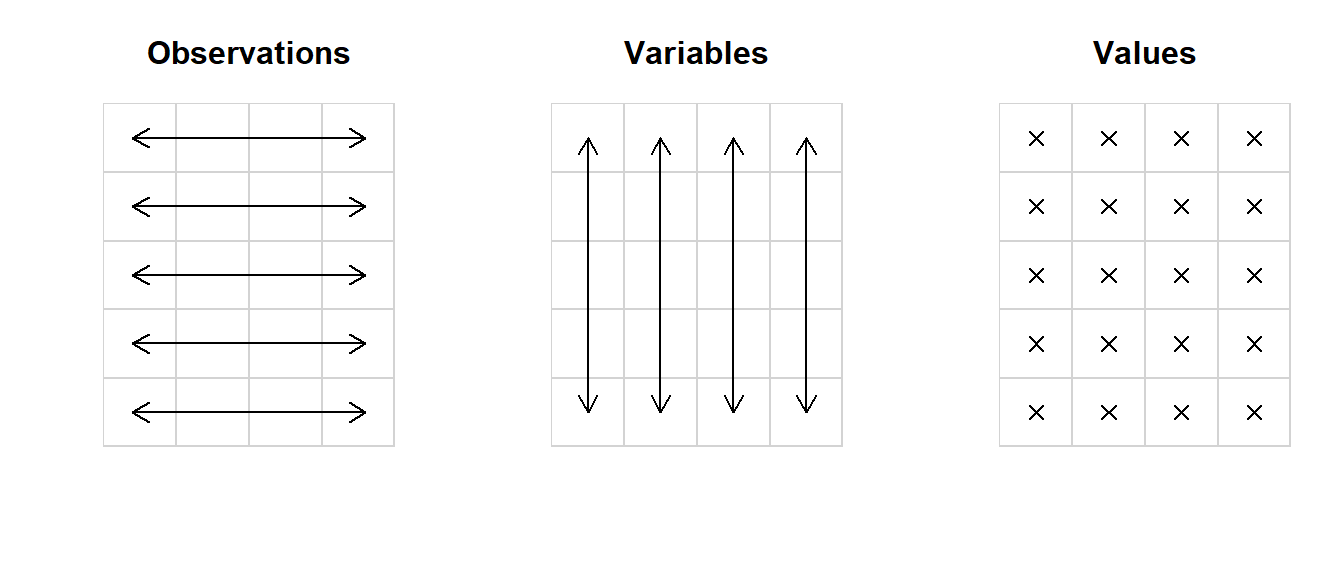
\includegraphics{Tutorials_files/figure-latex/unnamed-chunk-80-1.pdf}
\caption{\label{fig:unnamed-chunk-80}The basic principle of tidy data. This data set has 5 observations of 4 variables.}
\end{figure}

Good example

The \texttt{iris} data set (preinstalled with R) is in tidy format:

\begin{table}

\caption{\label{tab:unnamed-chunk-81}The first 5 rows of the <tt>iris</tt> data set. Each row is a flower and each column a property.}
\centering
\fontsize{11}{13}\selectfont
\begin{tabular}[t]{c|c|c|c|c}
\hline
Sepal.Length & Sepal.Width & Petal.Length & Petal.Width & Species\\
\hline
5.1 & 3.5 & 1.4 & 0.2 & setosa\\
\hline
4.9 & 3.0 & 1.4 & 0.2 & setosa\\
\hline
4.7 & 3.2 & 1.3 & 0.2 & setosa\\
\hline
4.6 & 3.1 & 1.5 & 0.2 & setosa\\
\hline
5.0 & 3.6 & 1.4 & 0.2 & setosa\\
\hline
... & ... & ... & ... & ...\\
\hline
\end{tabular}
\end{table}

Here, the rows each represent one observation (a distinct flower), and the columns represent the variables measured/recorded (physical dimensions and species).

Bad example

A common deviation from tidy format is to represent groups as columns:

\begin{table}

\caption{\label{tab:unnamed-chunk-82}Systolic blood pressure (SBP) of 10 individuals. <font color = 'red'>(untidy)</font>}
\centering
\fontsize{11}{13}\selectfont
\begin{tabular}[t]{c|c}
\hline
women & men\\
\hline
114 & 123\\
\hline
121 & 117\\
\hline
125 & 117\\
\hline
108 & 117\\
\hline
122 & 116\\
\hline
\end{tabular}
\end{table}

Do you have different groups? Time points? Replicates of the experiment? Then try to adhere to the same principle: Columns are variables. Simply add a variable that indicates which group/time point/replicate this observation belongs to:

\begin{table}

\caption{\label{tab:unnamed-chunk-83}Sex and systolic blood pressure (SBP) of 10 individuals. <font color = 'blue'>(tidy)</font>}
\centering
\fontsize{11}{13}\selectfont
\begin{tabular}[t]{c|c}
\hline
sex & SBP\\
\hline
female & 114\\
\hline
female & 121\\
\hline
female & 125\\
\hline
female & 108\\
\hline
female & 122\\
\hline
male & 123\\
\hline
male & 117\\
\hline
male & 117\\
\hline
male & 117\\
\hline
male & 116\\
\hline
\end{tabular}
\end{table}

Converting to tidy format

If you have data split by group/time point/replicate here is how you can convert it to tidy format:

\begin{Shaded}
\begin{Highlighting}[]
\CommentTok{\# The untidy data set}
\NormalTok{Untidy}
\end{Highlighting}
\end{Shaded}

\begin{verbatim}
##   women men
## 1   114 123
## 2   121 117
## 3   125 117
## 4   108 117
## 5   122 116
\end{verbatim}

\begin{Shaded}
\begin{Highlighting}[]
\CommentTok{\# Convert by hand}
\NormalTok{Tidy }\OtherTok{\textless{}{-}} \FunctionTok{data.frame}\NormalTok{(}
  \AttributeTok{sex =} \FunctionTok{rep}\NormalTok{(}\FunctionTok{c}\NormalTok{(}\StringTok{"female"}\NormalTok{, }\StringTok{"male"}\NormalTok{), }\AttributeTok{each =} \FunctionTok{nrow}\NormalTok{(Untidy)),}
  \AttributeTok{SBP =} \FunctionTok{c}\NormalTok{(Untidy}\SpecialCharTok{$}\NormalTok{women, Untidy}\SpecialCharTok{$}\NormalTok{men)}
\NormalTok{)}

\CommentTok{\# Convert using a package (install if missing)}
\FunctionTok{library}\NormalTok{(}\StringTok{"reshape2"}\NormalTok{)}
\FunctionTok{melt}\NormalTok{(Untidy)}
\end{Highlighting}
\end{Shaded}

\begin{verbatim}
##    variable value
## 1     women   114
## 2     women   121
## 3     women   125
## 4     women   108
## 5     women   122
## 6       men   123
## 7       men   117
## 8       men   117
## 9       men   117
## 10      men   116
\end{verbatim}

If you have a simple data set like the one shown here, converting with the package \texttt{reshape2} is easiest. Converting by hand may be slightly more work, but I prefer it because you can easily see what's going on, add more variables if needed, etc.

\hypertarget{separate-data-entry-analysis}{%
\section{Separate Data Entry \& Analysis}\label{separate-data-entry-analysis}}

Spreadsheet software like Excel or Google Sheets is great for easy data entry. A well-designed spreadsheet can even partially protect against errors, by limiting what values are allowed in certain columns (e.g., how \texttt{Species} is restricted \href{https://docs.google.com/spreadsheets/d/1dcblrkYrCO5lz7akSCkguYSWHfGxfJh2f6Pg2B8Q9ck/edit?pli=1\#gid=1478490863}{here}).\footnote{In Google Sheets, you can do this by going to \textbf{Data} \textgreater{} \textbf{Data validation}.}

Beware `intelligent' conversions

Programming requires exact precision in syntax, which can be very frustrating for beginners. To address this, many programs try to intelligently interpret your input:

\begin{figure}

\includegraphics[width=1\linewidth]{figures/typo} \caption{My hasty attempt to figure out which clothes to wear to work.}\label{fig:unnamed-chunk-85}
\end{figure}

While this usually a good thing, Excel does many such corrections without notice, and some even irreversibly. This can have serious repercussions for scientific research. For example, a 2016 article found widespread errors in gene names due to autocorrected Excel input.\citep{genenameerrors} Always check whether your input is correctly interpreted, or change the data type to ``text'' instead of ``general'' for everything you enter.

Once the data are correctly entered into some spreadsheet software (Excel, Google Sheets), this is where the data entry ends. Do not add any markup, coloring, notes, figures, or tables.

As a general principle, \textbf{raw data should never be edited}, nor should it be cluttered with additional information. This does not belong in your raw data, but either in a \protect\hyperlink{metadata}{meta data} file, or in some separate file for analysis that takes the raw data file as input.

Some additional guidelines for tidy data entry include:

\begin{itemize}
\tightlist
\item
  Avoid empty rows or columns for spacing, start at row 1, column 1;
\item
  Avoid the `merge cells' option, this breaks the row/column format;
\item
  Limit a spreadsheet to one data set. Adding multiple data sets to one sheet may look like you have more oversight in \emph{Excel}, but it makes any downstream analysis more convoluted.
\end{itemize}

\hypertarget{excel-is-not-statistical-software}{%
\subsection*{Excel Is Not Statistical Software}\label{excel-is-not-statistical-software}}
\addcontentsline{toc}{subsection}{Excel Is Not Statistical Software}

Even if you do create a separate file to explore/analyze your data, I still advice against using Excel for this, for the following reasons:

A history of inaccuracies

Excel has long been a program ridden with computational inaccuracies and slow to correct its mistakes.

Non-trivial errors in the calculation of discrete probability distributions, as well as severe limitations of its random number generator (\texttt{RAND()}) were found in Excel 1997,\citep{Excel1997a, Excel1997b} exacerbated in Excel 2000/XP,\citep{Excel2000} and only partially addressed in Excel 2003, while simultaneously introducing new problems.\citep{Excel2003a, Excel2003b} Perhaps unsurprisingly then, Excel 2007 still failed some of the same accuracy tests in use since 1998.\citep{Excel2007}

By the time Excel 2010 was released, persisting issues with the computation of probabilities and quantiles had been addressed, and the \texttt{RAND()} function had improved.\citep{Excel2010} Nevertheless, the authors of a paper reviewing Excel 2010 concluded:

\begin{quote}
{[}W{]}ithout a prompt reaction from Microsoft, the already very critical view against using spreadsheets for doing any statistical analysis {[}\ldots{]} will be even more justified. \textbf{It is standard practice for software developers to fix errors quickly and correctly. Microsoft has fixed the errors in the statistical procedures of Excel neither quickly nor correctly.} The recent improvements reported in this paper should not hide the fact that Microsoft is still marketing a product that contains known errors.
\end{quote}

I have emphasized the part that summarizes this section. Excel is proprietary software from a developer that cares little for its statistical accuracy. In contrast, R, Python, Julia and the likes are free \& open source (meaning anyone can view the source code).

Few new articles have since been published on this issue---presumably because R and Python have since become the \emph{de facto} industry standard for statistical analysis.

Lack of serious modeling options

If statistics were a toolbox, then Excel would be a hammer. Yes, you can do a lot with it, but if you're trying to cut something in half, or insert a screw, maybe use a different tool. Excel has add-ins, but these are neither open source, nor curated.

As of writing, R has 18,834 free, open source packages, offering anything from statistical tests, models, machine learning, visualization (\texttt{base}, \texttt{ggplot2}, \texttt{plotly}), literate programming (\texttt{rmarkdown}, \texttt{quarto}), presentations (e.g., \texttt{xaringan}), paper writing (\texttt{rticles}), book authoring (\texttt{bookdown}), app and dashboard development (\texttt{shiny}), and even interfaces to state-of-the-art deep learning frameworks (e.g., \texttt{tensorflow}, \texttt{keras}).

Computations are opaque

Analyses performed in Excel consist of cells with formulas referring to other (ranges of) cells. This is not a problem for simple operations, like adding or subtracting two columns. But in actual analysis, there will be many such steps, and Excel `code' becomes much harder to read than other programming languages, since you can only view the contents of one cell at a time.

The worst offenders are large Excel sheets with both data and computations, requiring not only that you trace back the operations performed in multiple cells, but also that you scroll between (often distant) locations in the sheet. Bugs \emph{will} appear in large analyses and it is needlessly difficult to trace the origin of mistakes.

Excel is also slow, especially in files combining data and analysis; it is paid software, requiring a license; and its `arrange cells however you see fit' approach, makes analyses much harder to reproduce.

If you want an easy interface to enter your data, Excel is great software. Any elaborate analyses in Excel though, are inefficient at best and severely limited at worst.

\hypertarget{metadata}{%
\section{Meta Data}\label{metadata}}

To help keep variable names short, to include the unit of measurement, to explain how something was measured, or to provide other relevant comments about the data, you can keep a meta data file (or sheet). An example can be found \href{https://docs.google.com/spreadsheets/d/1dcblrkYrCO5lz7akSCkguYSWHfGxfJh2f6Pg2B8Q9ck/edit?pli=1\#gid=322816193}{here}.

Meta data means \emph{data about data}. If you take a picture with your phone, meta data contains information about how the picture was taken (shutter time, ISO, etc.), or where the picture was taken. Naturally, you do not want this information pasted onto the picture itself. In a similar vein, you should not include comments about the data, in the raw data itself. This is why you should keep a separate file for meta data.

\hypertarget{csv}{%
\section{Reading Data as CSV}\label{csv}}

Why this format?

Saving into CSV format automatically removes any content statistical software cannot read anyway, like figures and coloring. This file format is suitable for most sizes of data commonly encountered in the life sciences (anything that still fits into RAM on an ordinary computer).

For very large data sets, there are special high-performance file types, like \href{https://en.wikipedia.org/wiki/Hierarchical_Data_Format\#HDF5}{HDF5} or \href{https://en.wikipedia.org/wiki/Apache_Parquet}{parquet}. However, these offer little to no benefit for the small-sized data sets used in the tutorials here.

Setting up your working directory

\begin{itemize}
\tightlist
\item
  Save the data in a folder;
\item
  Open RStudio and create a new R markdown file; (\textbf{File} \textgreater{} \textbf{New File} \textgreater{} \textbf{R Markdown})
\item
  Save your R markdown file to the same location as the data;
\item
  Set working directory to source file location. (\textbf{Session} \textgreater{} \textbf{Set Working Directory} \textgreater{} \textbf{To Source File Location})
\end{itemize}

Provided your working directory is set up correctly, you can read CSV files as follows:

\begin{Shaded}
\begin{Highlighting}[]
\NormalTok{DF }\OtherTok{\textless{}{-}} \FunctionTok{read.csv}\NormalTok{(}\StringTok{"NameOfYourFile.csv"}\NormalTok{)}
\end{Highlighting}
\end{Shaded}

Here, \texttt{DF} is an arbitrary name. I use it because it is short (you will be typing this name a lot) and because it is an abbreviation of `data frame', so it keeps code easy to read for others and your future self.

To check that your data has been read correctly by the software, try one of the following:

\begin{Shaded}
\begin{Highlighting}[]
\FunctionTok{str}\NormalTok{(DF)}
\FunctionTok{summary}\NormalTok{(DF)}
\FunctionTok{head}\NormalTok{(DF)}
\FunctionTok{tail}\NormalTok{(DF)}
\end{Highlighting}
\end{Shaded}

What it should look like

The \texttt{str} function displays the structure of the object. In case your file is in tidy format and read correctly, it will look something like this:

\begin{Shaded}
\begin{Highlighting}[]
\FunctionTok{str}\NormalTok{(iris)}
\end{Highlighting}
\end{Shaded}

\begin{verbatim}
## 'data.frame':    150 obs. of  5 variables:
##  $ Sepal.Length: num  5.1 4.9 4.7 4.6 5 5.4 4.6 5 4.4 4.9 ...
##  $ Sepal.Width : num  3.5 3 3.2 3.1 3.6 3.9 3.4 3.4 2.9 3.1 ...
##  $ Petal.Length: num  1.4 1.4 1.3 1.5 1.4 1.7 1.4 1.5 1.4 1.5 ...
##  $ Petal.Width : num  0.2 0.2 0.2 0.2 0.2 0.4 0.3 0.2 0.2 0.1 ...
##  $ Species     : Factor w/ 3 levels "setosa","versicolor",..: 1 1 1 1 1 1 1 1 1 1 ...
\end{verbatim}

More explanation

The first line tells us this object is a \texttt{data.frame} consisting of 150 observations (rows) and 5 variables (columns). It then tells us what kind of information those variables contain:

\begin{itemize}
\tightlist
\item
  \texttt{num}: Numeric (any number, stored as a \href{https://youtu.be/L8OYx1I8qNg}{floating point})
\item
  \texttt{int}: Integer (whole number)
\item
  \texttt{chr}: Character string
\item
  \texttt{Factor}: Categorical variable with a fixed number of levels
\item
  Some \href{https://adv-r.hadley.nz/vectors-chap.html\#s3-atomic-vectors}{less common ones}.
\end{itemize}

In the example shown here, the data has been read correctly, because numbers show as \texttt{num} and the flower species shows as \texttt{Factor}. If your factor shows up as a character (\texttt{chr}), you can convert it as follows:

\begin{Shaded}
\begin{Highlighting}[]
\NormalTok{DF}\SpecialCharTok{$}\NormalTok{x }\OtherTok{\textless{}{-}} \FunctionTok{factor}\NormalTok{(DF}\SpecialCharTok{$}\NormalTok{x)}
\end{Highlighting}
\end{Shaded}

Where \texttt{x} is the name of the variable you want to convert to factor.

The \texttt{summary} shows some summary statistics for numeric variables, and counts of categories for factors:

\begin{Shaded}
\begin{Highlighting}[]
\FunctionTok{summary}\NormalTok{(iris)}
\end{Highlighting}
\end{Shaded}

\begin{verbatim}
##   Sepal.Length    Sepal.Width     Petal.Length    Petal.Width   
##  Min.   :4.300   Min.   :2.000   Min.   :1.000   Min.   :0.100  
##  1st Qu.:5.100   1st Qu.:2.800   1st Qu.:1.600   1st Qu.:0.300  
##  Median :5.800   Median :3.000   Median :4.350   Median :1.300  
##  Mean   :5.843   Mean   :3.057   Mean   :3.758   Mean   :1.199  
##  3rd Qu.:6.400   3rd Qu.:3.300   3rd Qu.:5.100   3rd Qu.:1.800  
##  Max.   :7.900   Max.   :4.400   Max.   :6.900   Max.   :2.500  
##        Species  
##  setosa    :50  
##  versicolor:50  
##  virginica :50  
##                 
##                 
## 
\end{verbatim}

More explanation

For numeric variables, the minimum, first 25\%, first 50\% (median), the mean (average), first 75\% and the maximum are shown. This provides some basic indication of the distribution of the data, and it may point to potential outliers if the minimum or maximum are unrealistically far away.

For factors, the counts of categories are useful to see whether the data are balanced (same number of observations per category).

Finally, \texttt{head} and \texttt{tail} show the first and last rows of the data, respectively (6 rows by default):

\begin{Shaded}
\begin{Highlighting}[]
\FunctionTok{head}\NormalTok{(iris)}
\end{Highlighting}
\end{Shaded}

\begin{verbatim}
##   Sepal.Length Sepal.Width Petal.Length Petal.Width Species
## 1          5.1         3.5          1.4         0.2  setosa
## 2          4.9         3.0          1.4         0.2  setosa
## 3          4.7         3.2          1.3         0.2  setosa
## 4          4.6         3.1          1.5         0.2  setosa
## 5          5.0         3.6          1.4         0.2  setosa
## 6          5.4         3.9          1.7         0.4  setosa
\end{verbatim}

\begin{Shaded}
\begin{Highlighting}[]
\FunctionTok{tail}\NormalTok{(iris)}
\end{Highlighting}
\end{Shaded}

\begin{verbatim}
##     Sepal.Length Sepal.Width Petal.Length Petal.Width   Species
## 145          6.7         3.3          5.7         2.5 virginica
## 146          6.7         3.0          5.2         2.3 virginica
## 147          6.3         2.5          5.0         1.9 virginica
## 148          6.5         3.0          5.2         2.0 virginica
## 149          6.2         3.4          5.4         2.3 virginica
## 150          5.9         3.0          5.1         1.8 virginica
\end{verbatim}

My output looks different

First, make sure your data are in \protect\hyperlink{tidy}{tidy format}. That also means no empty rows before your data starts, no comments in cells where there is no data, etc.

If you're sure your data is in the right format, another very common issue is the \textbf{decimal separator}. In some countries (including The Netherlands), decimal numbers are separated with a comma, e.g.:

\[\begin{aligned}\text{Dutch style:} \quad 3 &- 0{,}1 = 2{,}9 \\
\text{English style:} \quad 3 &- 0.1 = 2.9
\end{aligned}\]

If you have a Dutch version of Excel, then CSV files are actually not separated by commas but semi-colons, because the software would otherwise not be able to tell new numbers and decimal numbers apart.

The solution for this is fortunately very simple, use read.csv2:

\begin{Shaded}
\begin{Highlighting}[]
\NormalTok{DF }\OtherTok{\textless{}{-}} \FunctionTok{read.csv2}\NormalTok{(}\StringTok{"NameOfYourFile.csv"}\NormalTok{)}
\end{Highlighting}
\end{Shaded}

If this too does not solve your problem, try copying the entire error message and searching for it online. Usually, there will have been someone else with the same problem on \href{stackoverflow.com}{StackOverflow}, so you can try the solutions offered there.

\hypertarget{Excel}{%
\section{Reading Data from Excel}\label{Excel}}

Reading data directly from Excel only works if R `understands' the file. An Excel file cluttered with figures or special functionality will not be readable, which is why I recommend just using \href{https://youtu.be/BGUqZc-Pb8w}{CSV} instead. Despite the drawbacks, experience shows that many people prefer to read data directly from Excel anyway, so I will demonstrate this too.

Setting up your working directory

\begin{itemize}
\tightlist
\item
  Save the data in a folder;
\item
  Open RStudio and create a new R markdown file; (\textbf{File} \textgreater{} \textbf{New File} \textgreater{} \textbf{R Markdown})
\item
  Save your R markdown file to the same location as the data;
\item
  Set working directory to source file location. (\textbf{Session} \textgreater{} \textbf{Set Working Directory} \textgreater{} \textbf{To Source File Location})
\end{itemize}

Provided your working directory is set up correctly, there are many ways to directly read your Excel file into R, for example:

\begin{Shaded}
\begin{Highlighting}[]
\CommentTok{\# Using readxl}
\FunctionTok{library}\NormalTok{(}\StringTok{"readxl"}\NormalTok{)}
\NormalTok{DF }\OtherTok{\textless{}{-}} \FunctionTok{read\_xlsx}\NormalTok{(}\StringTok{"NameOfYourFile.xlsx"}\NormalTok{, }\AttributeTok{sheet =} \DecValTok{1}\NormalTok{)}

\CommentTok{\# Using xlsx}
\FunctionTok{library}\NormalTok{(}\StringTok{"xlsx"}\NormalTok{)}
\NormalTok{DF }\OtherTok{\textless{}{-}} \FunctionTok{read.xlsx}\NormalTok{(}\StringTok{"NameOfYourFile.xlsx"}\NormalTok{, }\AttributeTok{sheetIndex =} \DecValTok{1}\NormalTok{)}

\CommentTok{\# Using fread}
\FunctionTok{library}\NormalTok{(}\StringTok{"data.table"}\NormalTok{)}
\NormalTok{DF }\OtherTok{\textless{}{-}} \FunctionTok{fread}\NormalTok{(}\AttributeTok{file =} \StringTok{"NameOfYourFile.xlsx"}\NormalTok{)}
\end{Highlighting}
\end{Shaded}

If you are already familiar with the syntax of one of these packages, there is no need to switch. If people send me Excel sheets, I usually use \texttt{readxl}. A more general and high-performance function is \texttt{fread} from the package \texttt{data.table}.

\hypertarget{references}{%
\chapter*{References}\label{references}}
\addcontentsline{toc}{chapter}{References}

  \bibliography{citations.bib}

\end{document}
